\section{Stability Plots \label{sec:appendix:stability}}

\subsection{$\fx=c$\label{sec:appendix:stability:fxc}}
\subsubsection{\mjj Asimov fluctuations, MG5 QCD in Asimov, MG5 QCD template}
\begin{figure}[H]
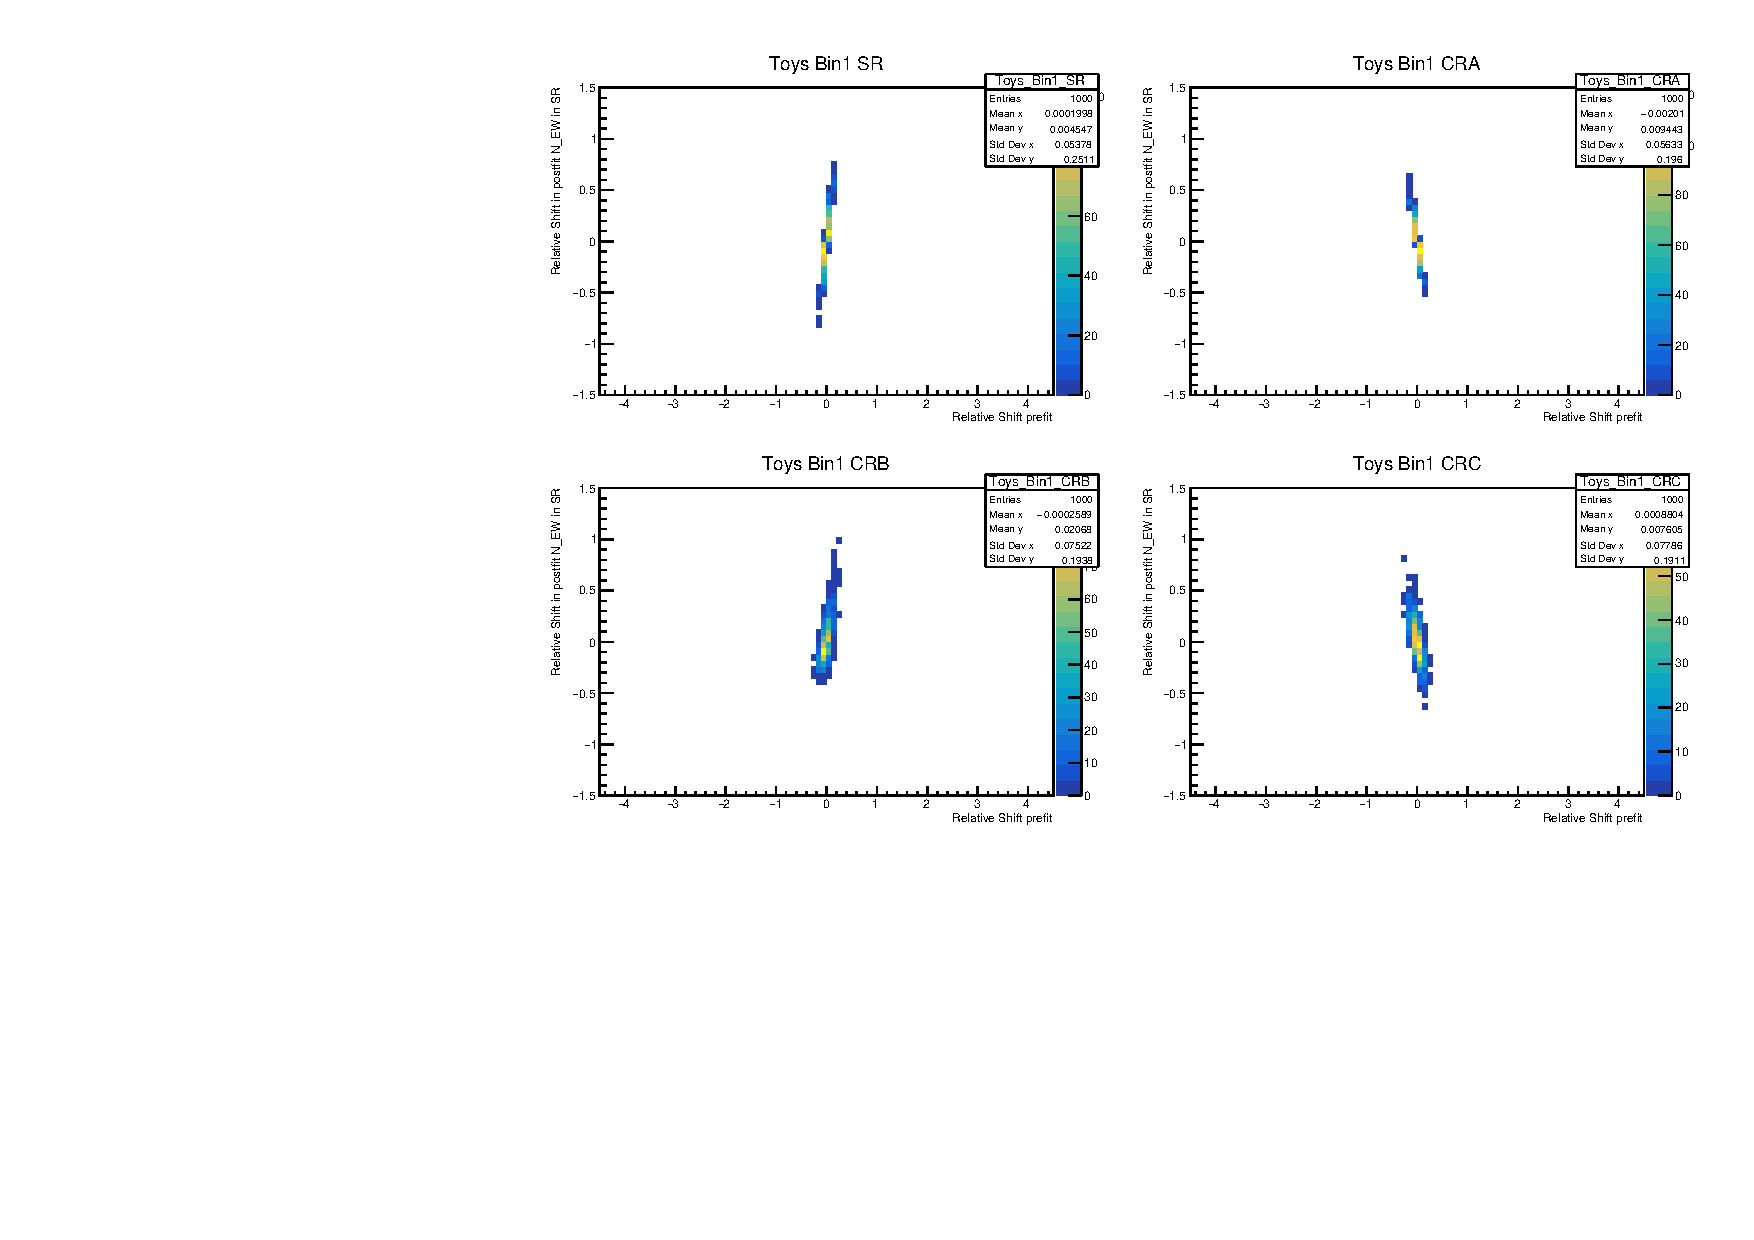
\includegraphics[width=\textwidth]{plots/diffx/instab/constfx/instabilities_mjj_QCD_Mgraph_Signal_Sh2211_BSDATASTATS_madgraphasimov_bin1.pdf}
\end{figure}
\begin{figure}[H]
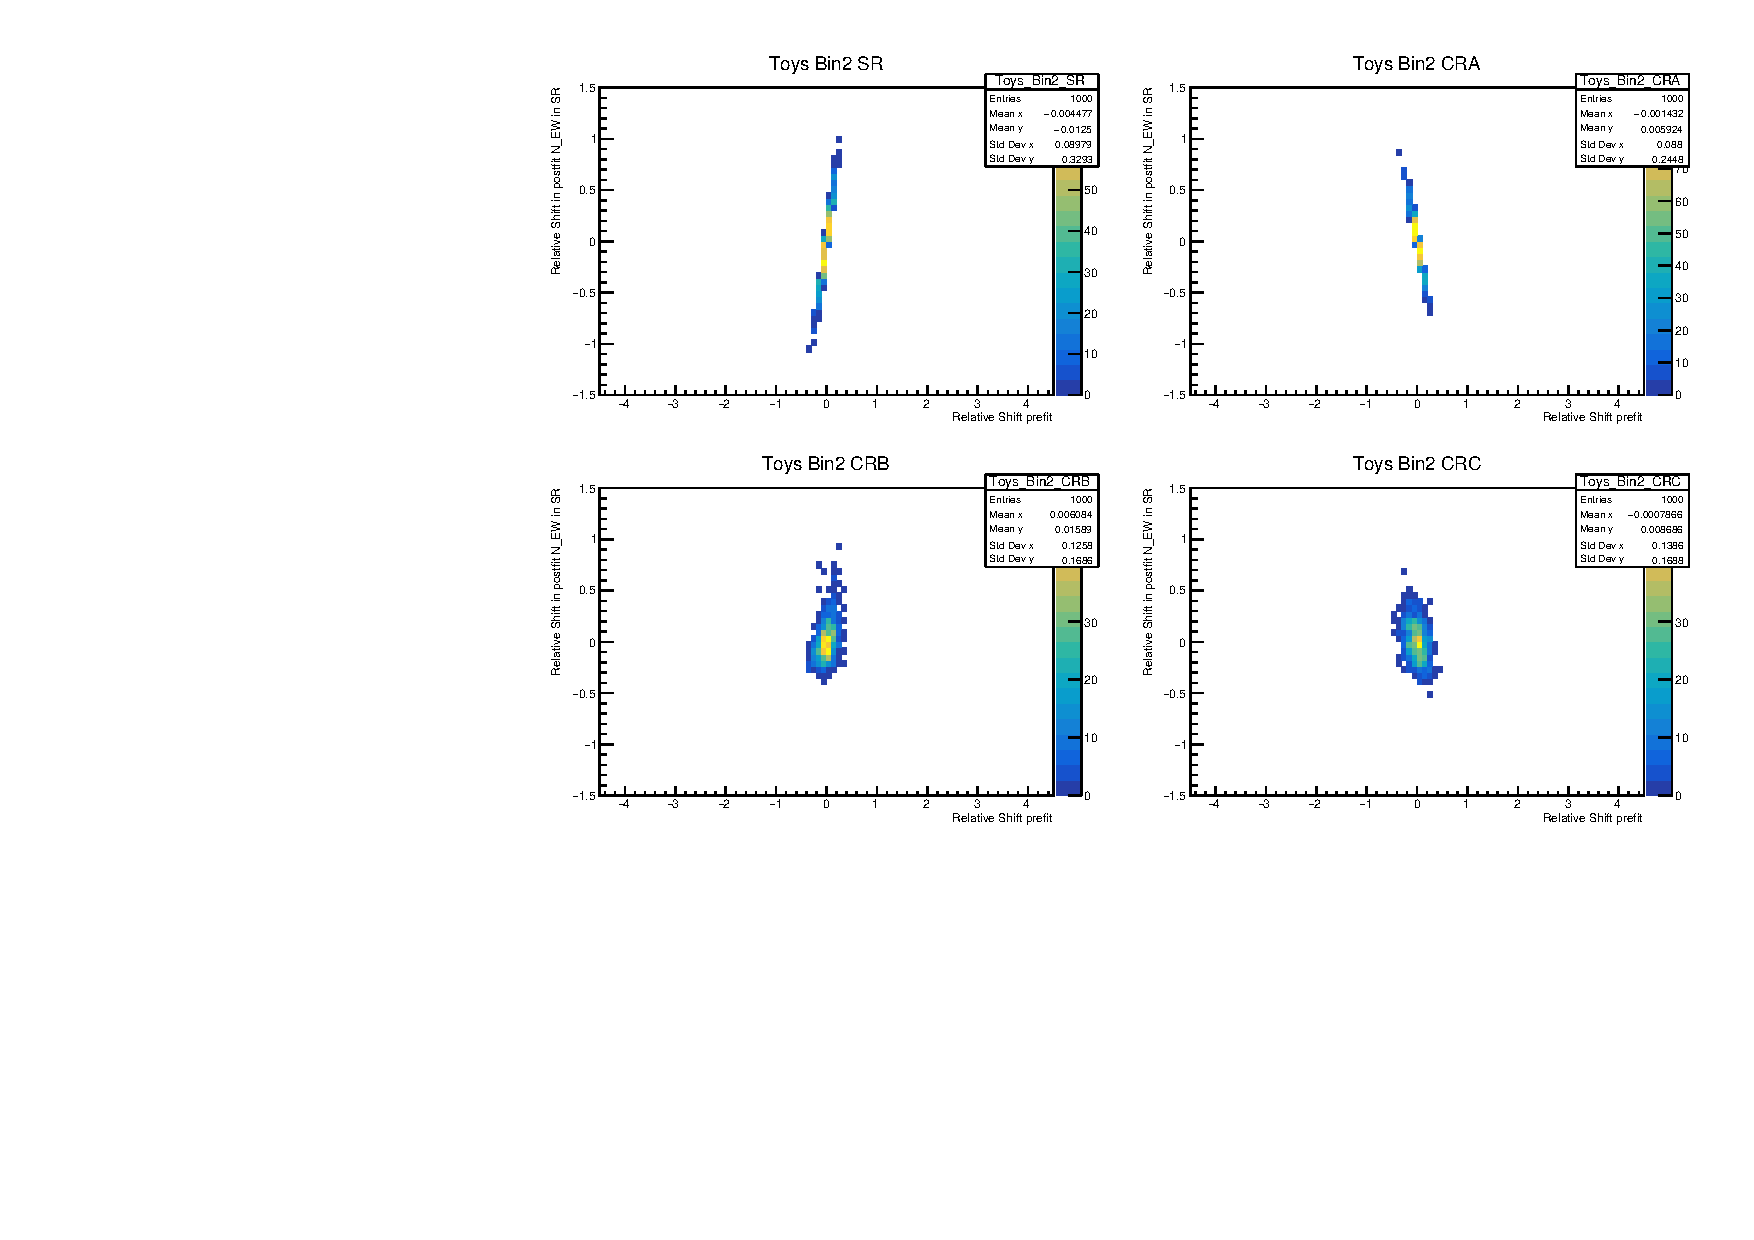
\includegraphics[width=\textwidth]{plots/diffx/instab/constfx/instabilities_mjj_QCD_Mgraph_Signal_Sh2211_BSDATASTATS_madgraphasimov_bin2.pdf}
\end{figure}
\begin{figure}[H]
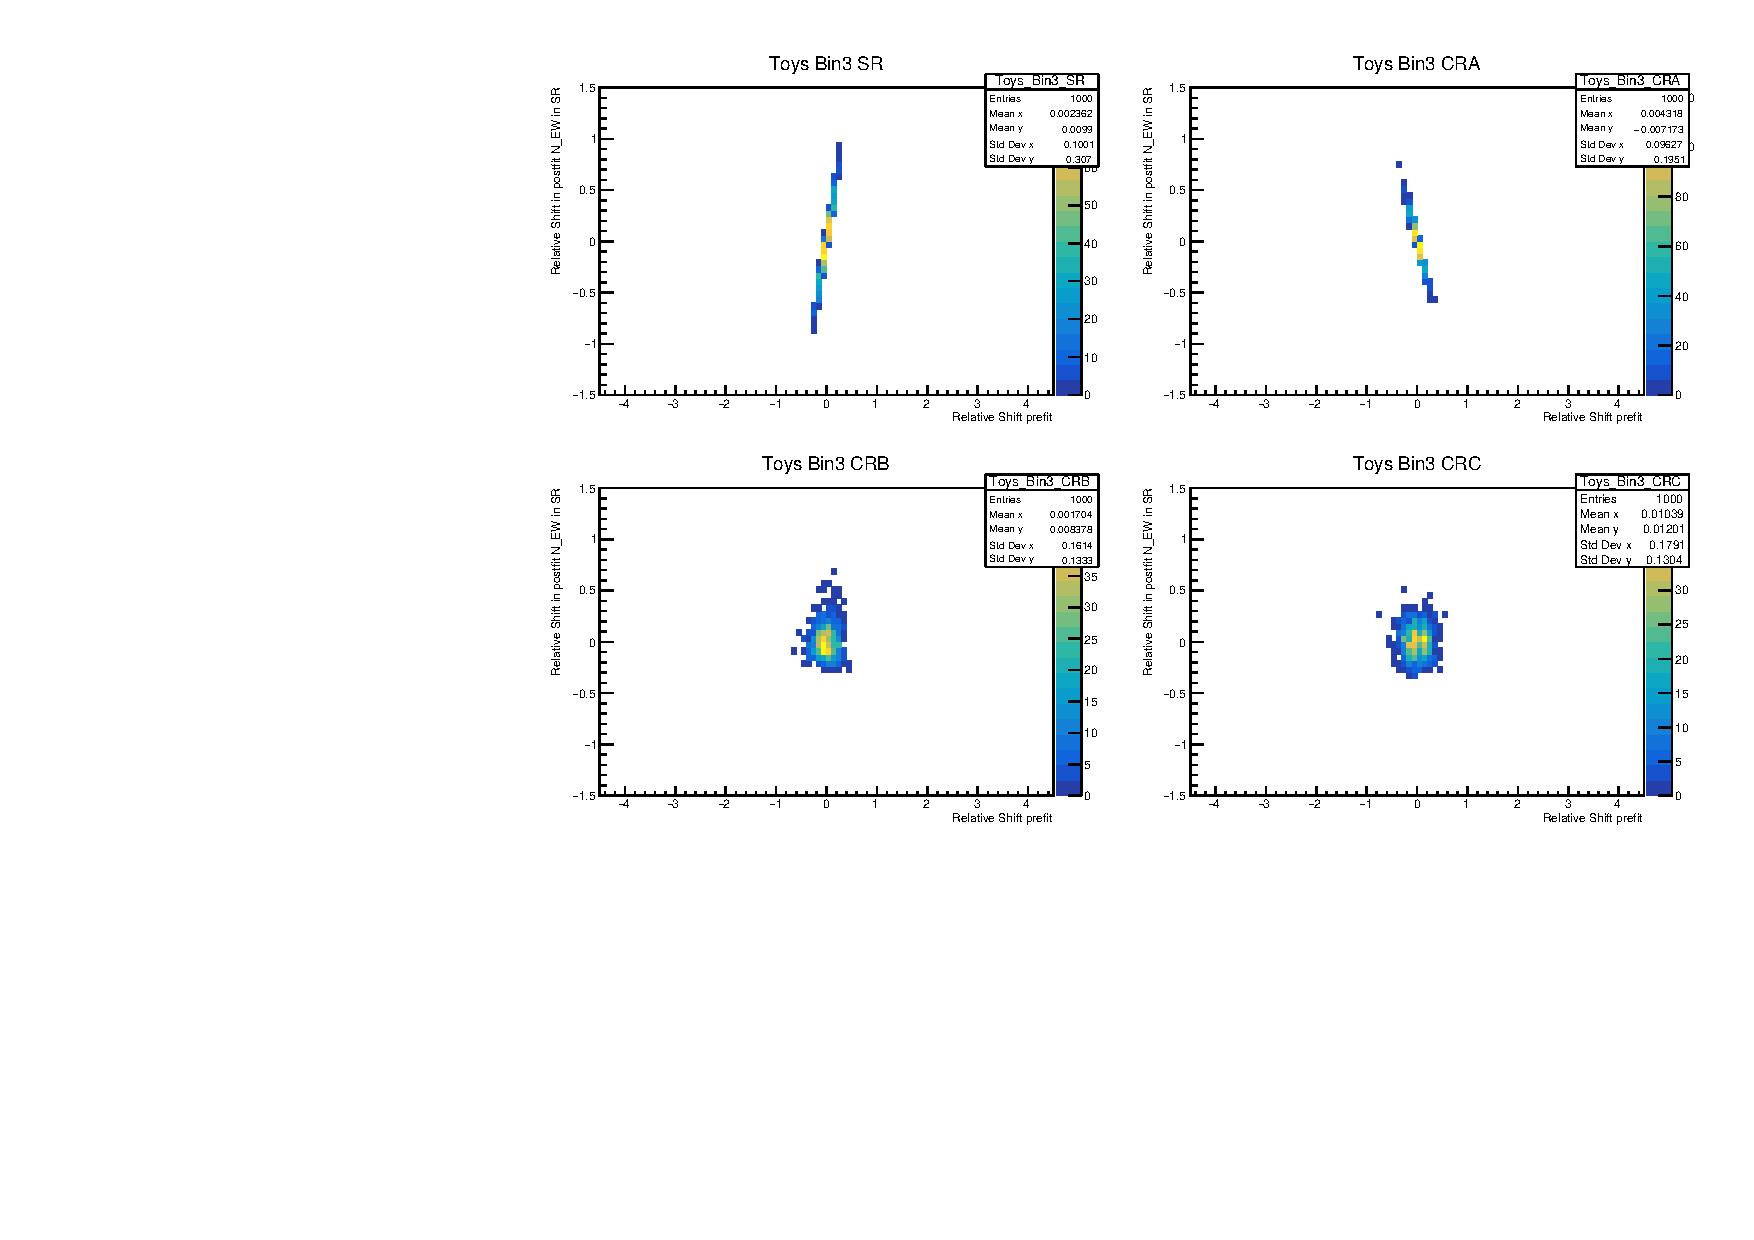
\includegraphics[width=\textwidth]{plots/diffx/instab/constfx/instabilities_mjj_QCD_Mgraph_Signal_Sh2211_BSDATASTATS_madgraphasimov_bin3.pdf}
\end{figure}
\begin{figure}[H]
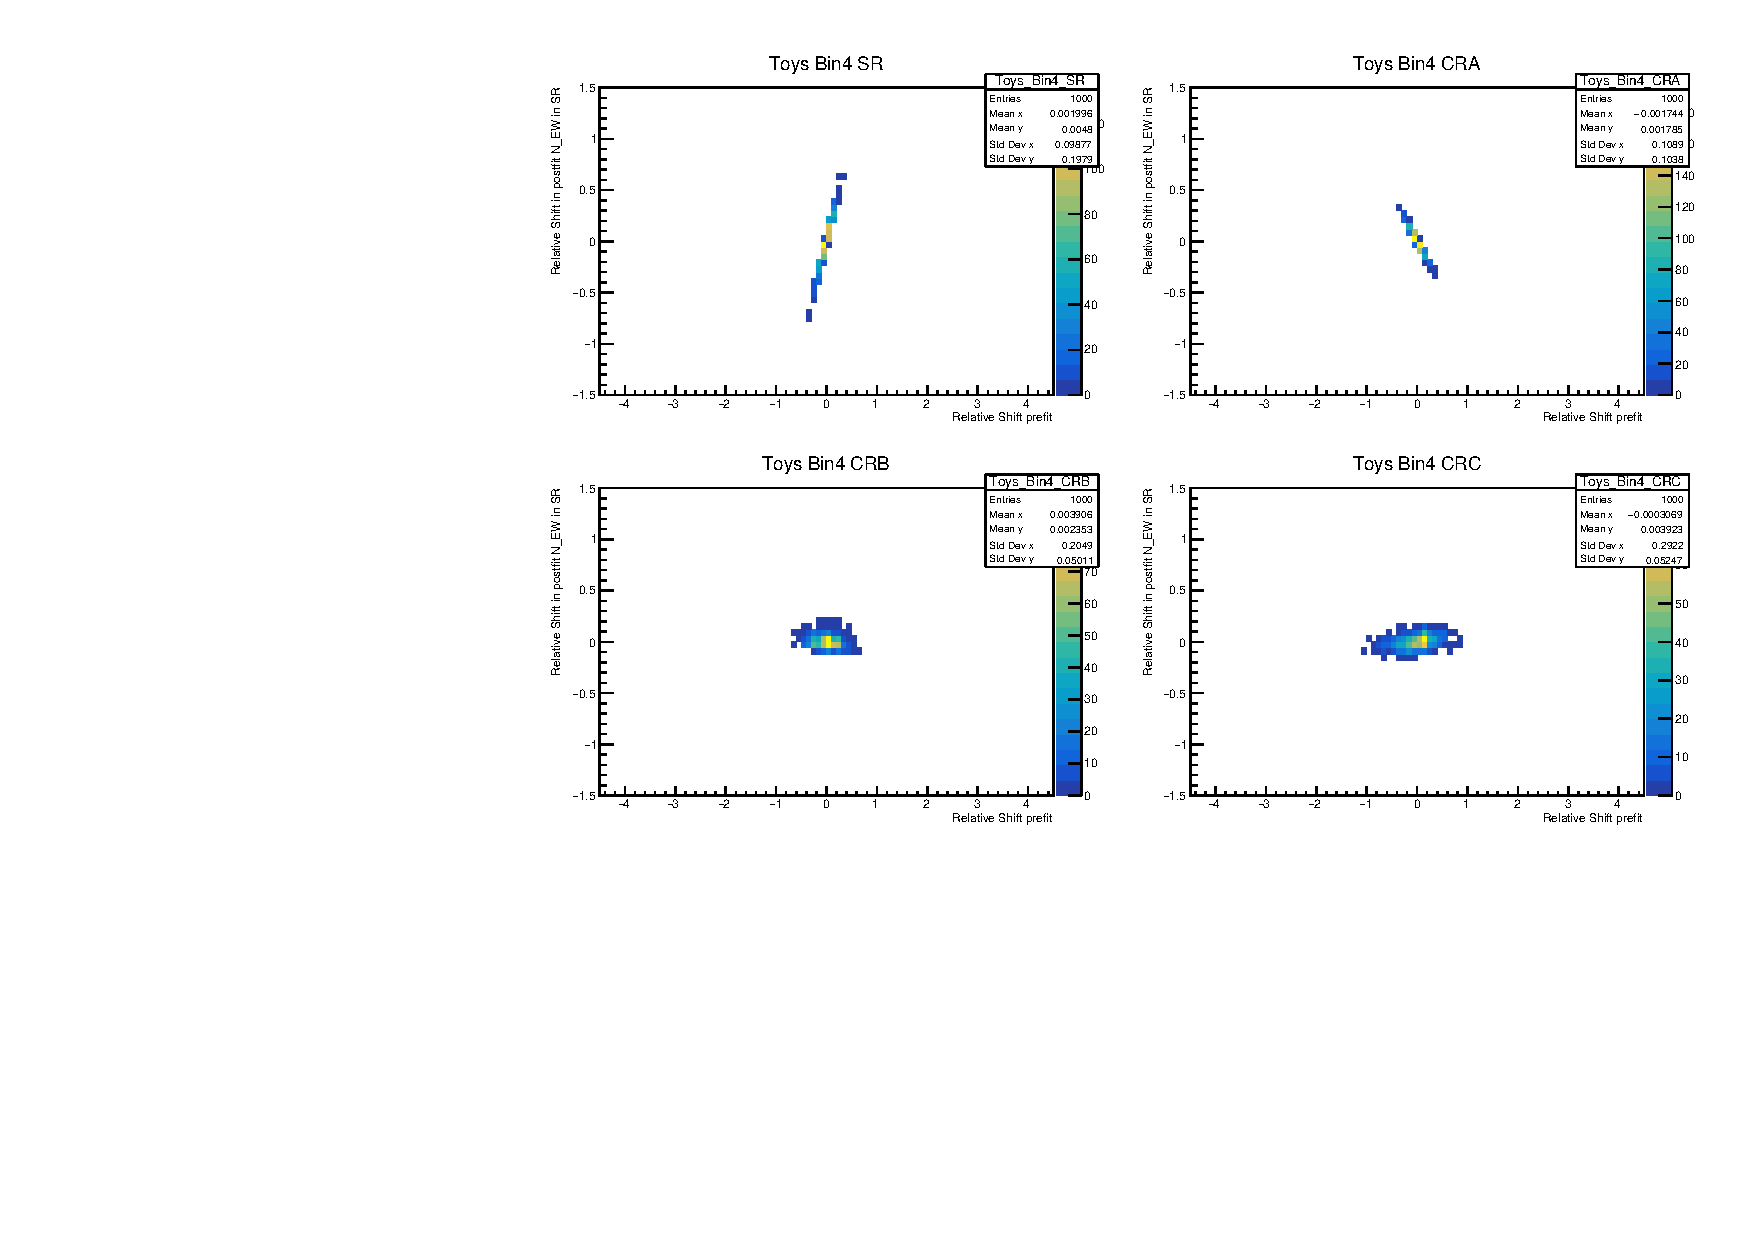
\includegraphics[width=\textwidth]{plots/diffx/instab/constfx/instabilities_mjj_QCD_Mgraph_Signal_Sh2211_BSDATASTATS_madgraphasimov_bin4.pdf}
\end{figure}

\subsubsection{\mjj Asimov fluctuations, Sherpa-2.2.11 QCD in Asimov, MG5 QCD template}
\begin{figure}[H]
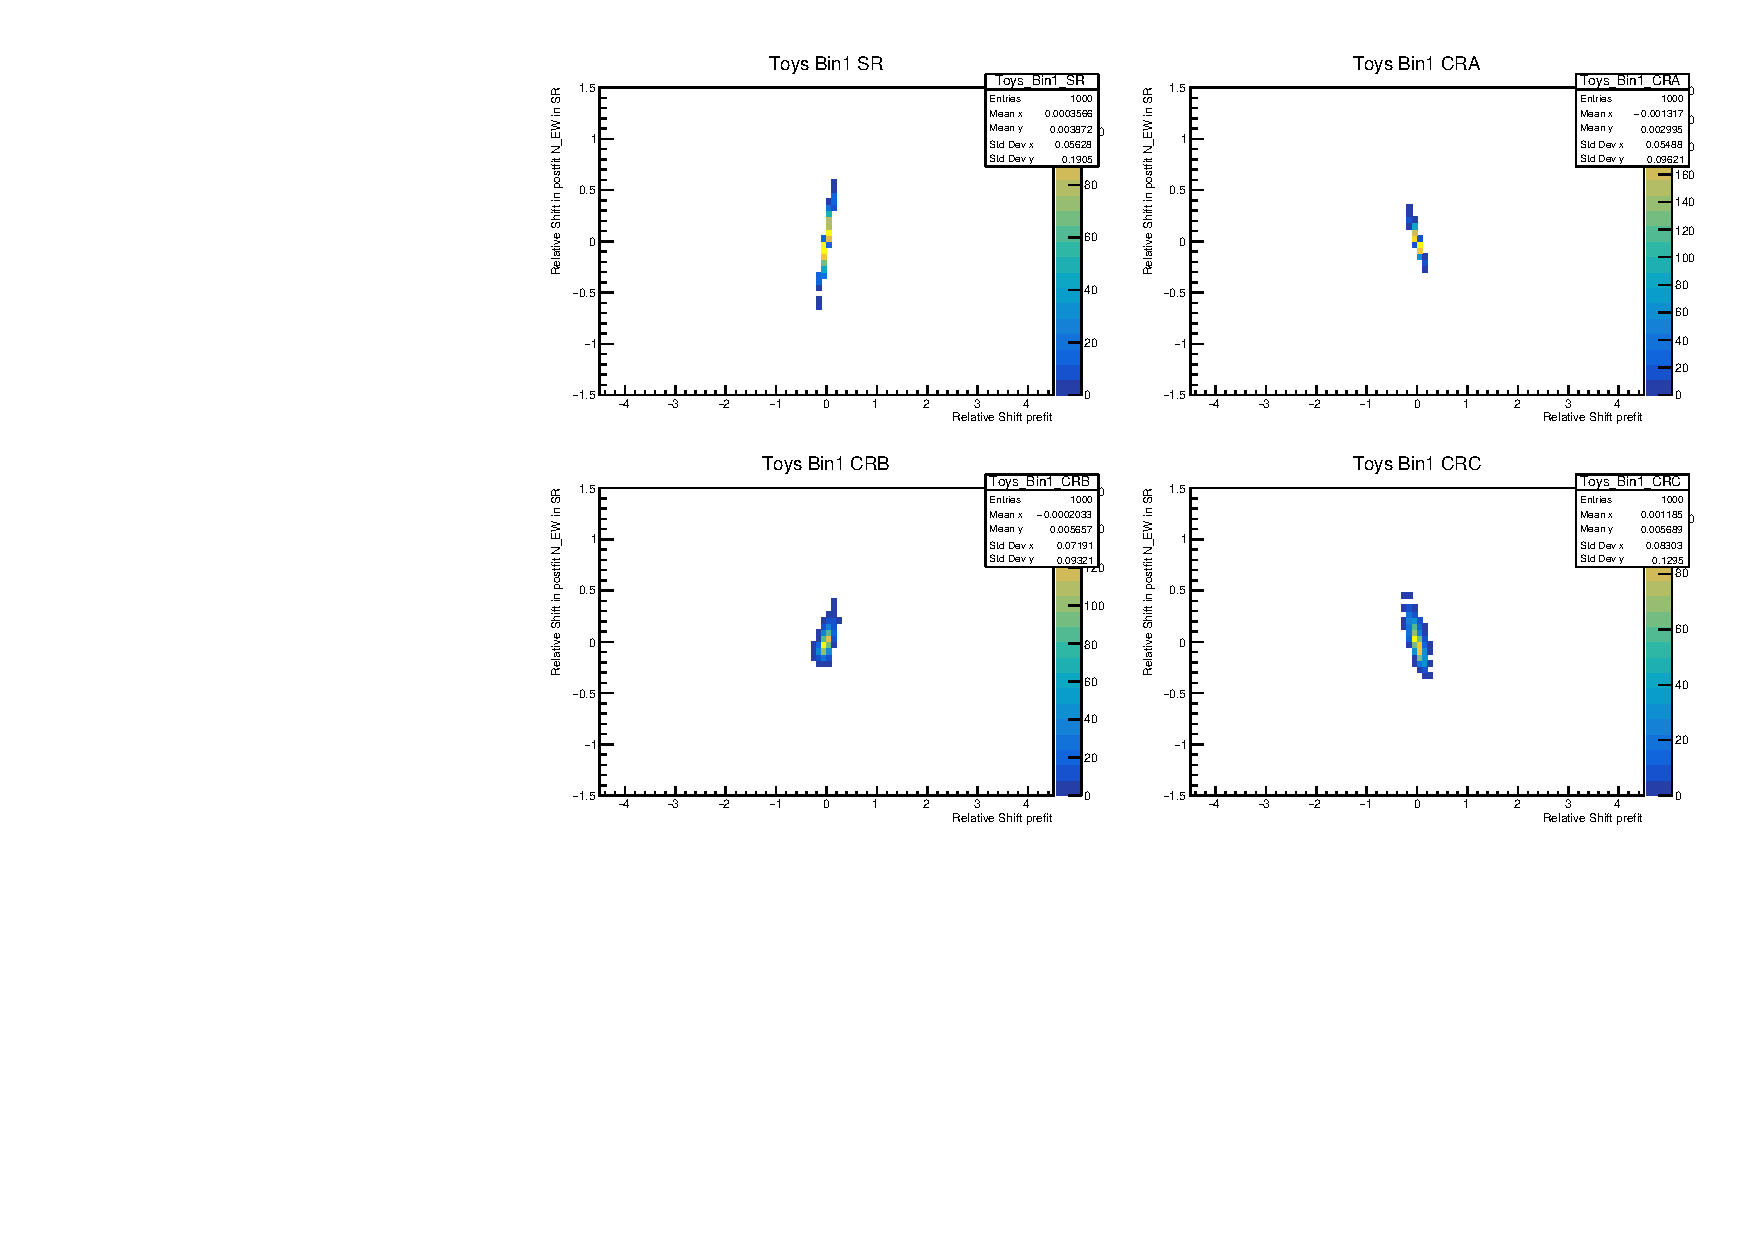
\includegraphics[width=\textwidth]{plots/diffx/instab/constfx/instabilities_mjj_QCD_Mgraph_Signal_Sh2211_BSDATASTATS_sherpaasimov_bin1.pdf}
\end{figure}
\begin{figure}[H]
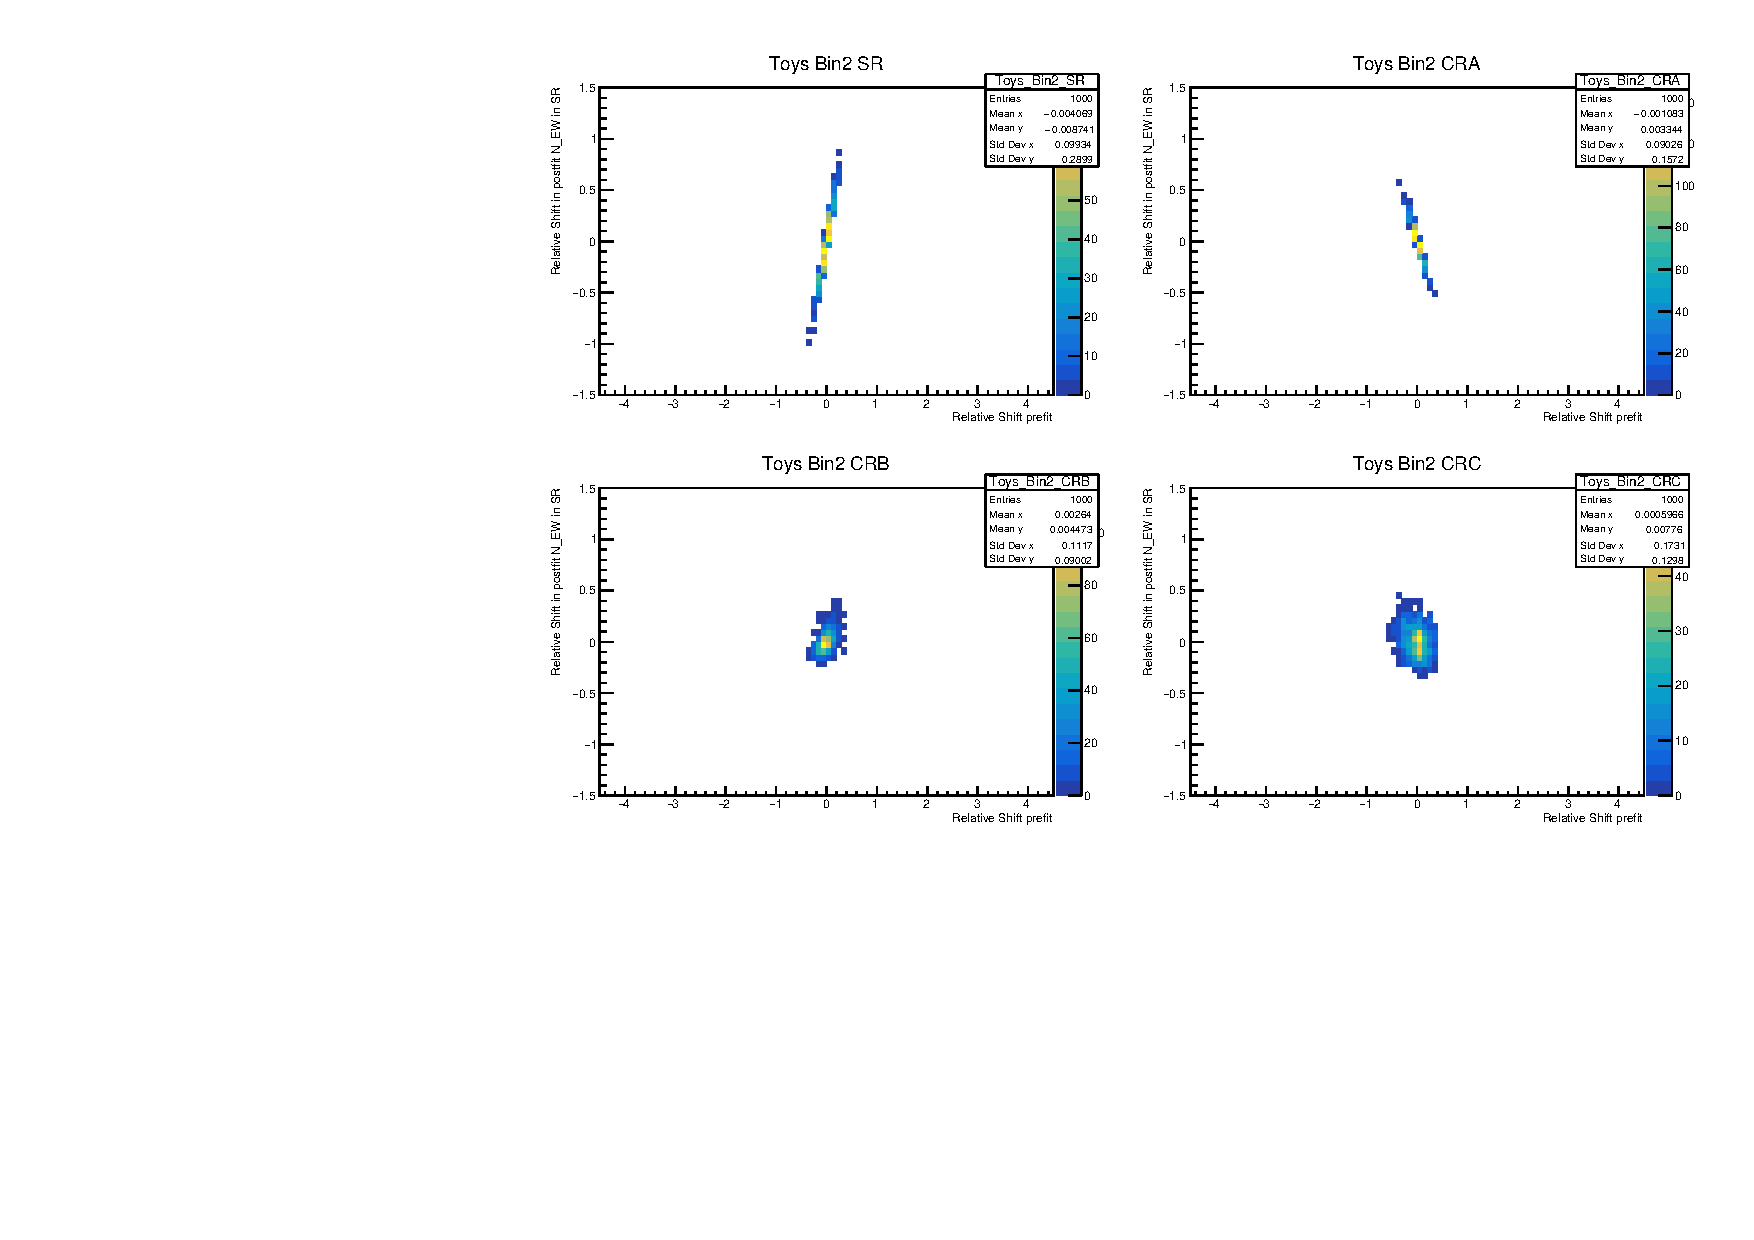
\includegraphics[width=\textwidth]{plots/diffx/instab/constfx/instabilities_mjj_QCD_Mgraph_Signal_Sh2211_BSDATASTATS_sherpaasimov_bin2.pdf}
\end{figure}
\begin{figure}[H]
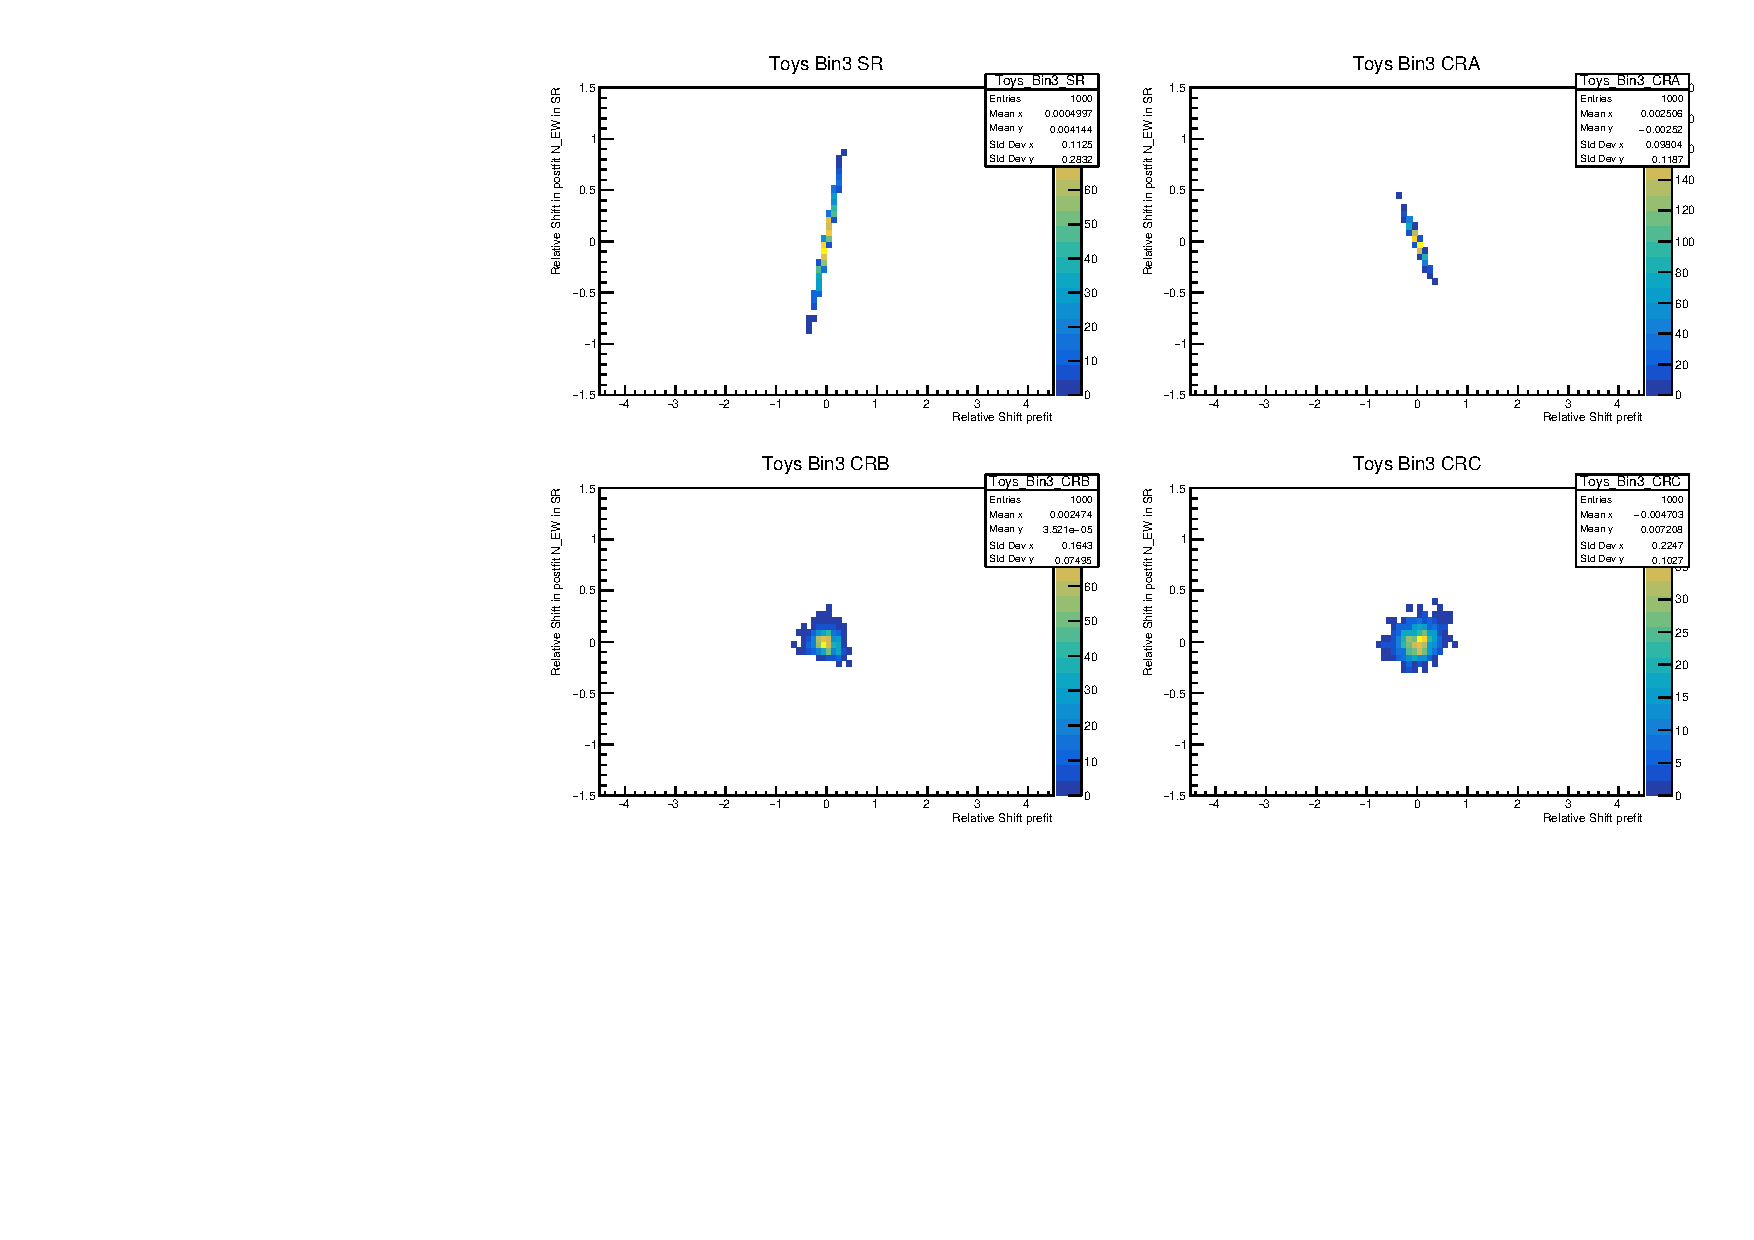
\includegraphics[width=\textwidth]{plots/diffx/instab/constfx/instabilities_mjj_QCD_Mgraph_Signal_Sh2211_BSDATASTATS_sherpaasimov_bin3.pdf}
\end{figure}
\begin{figure}[H]
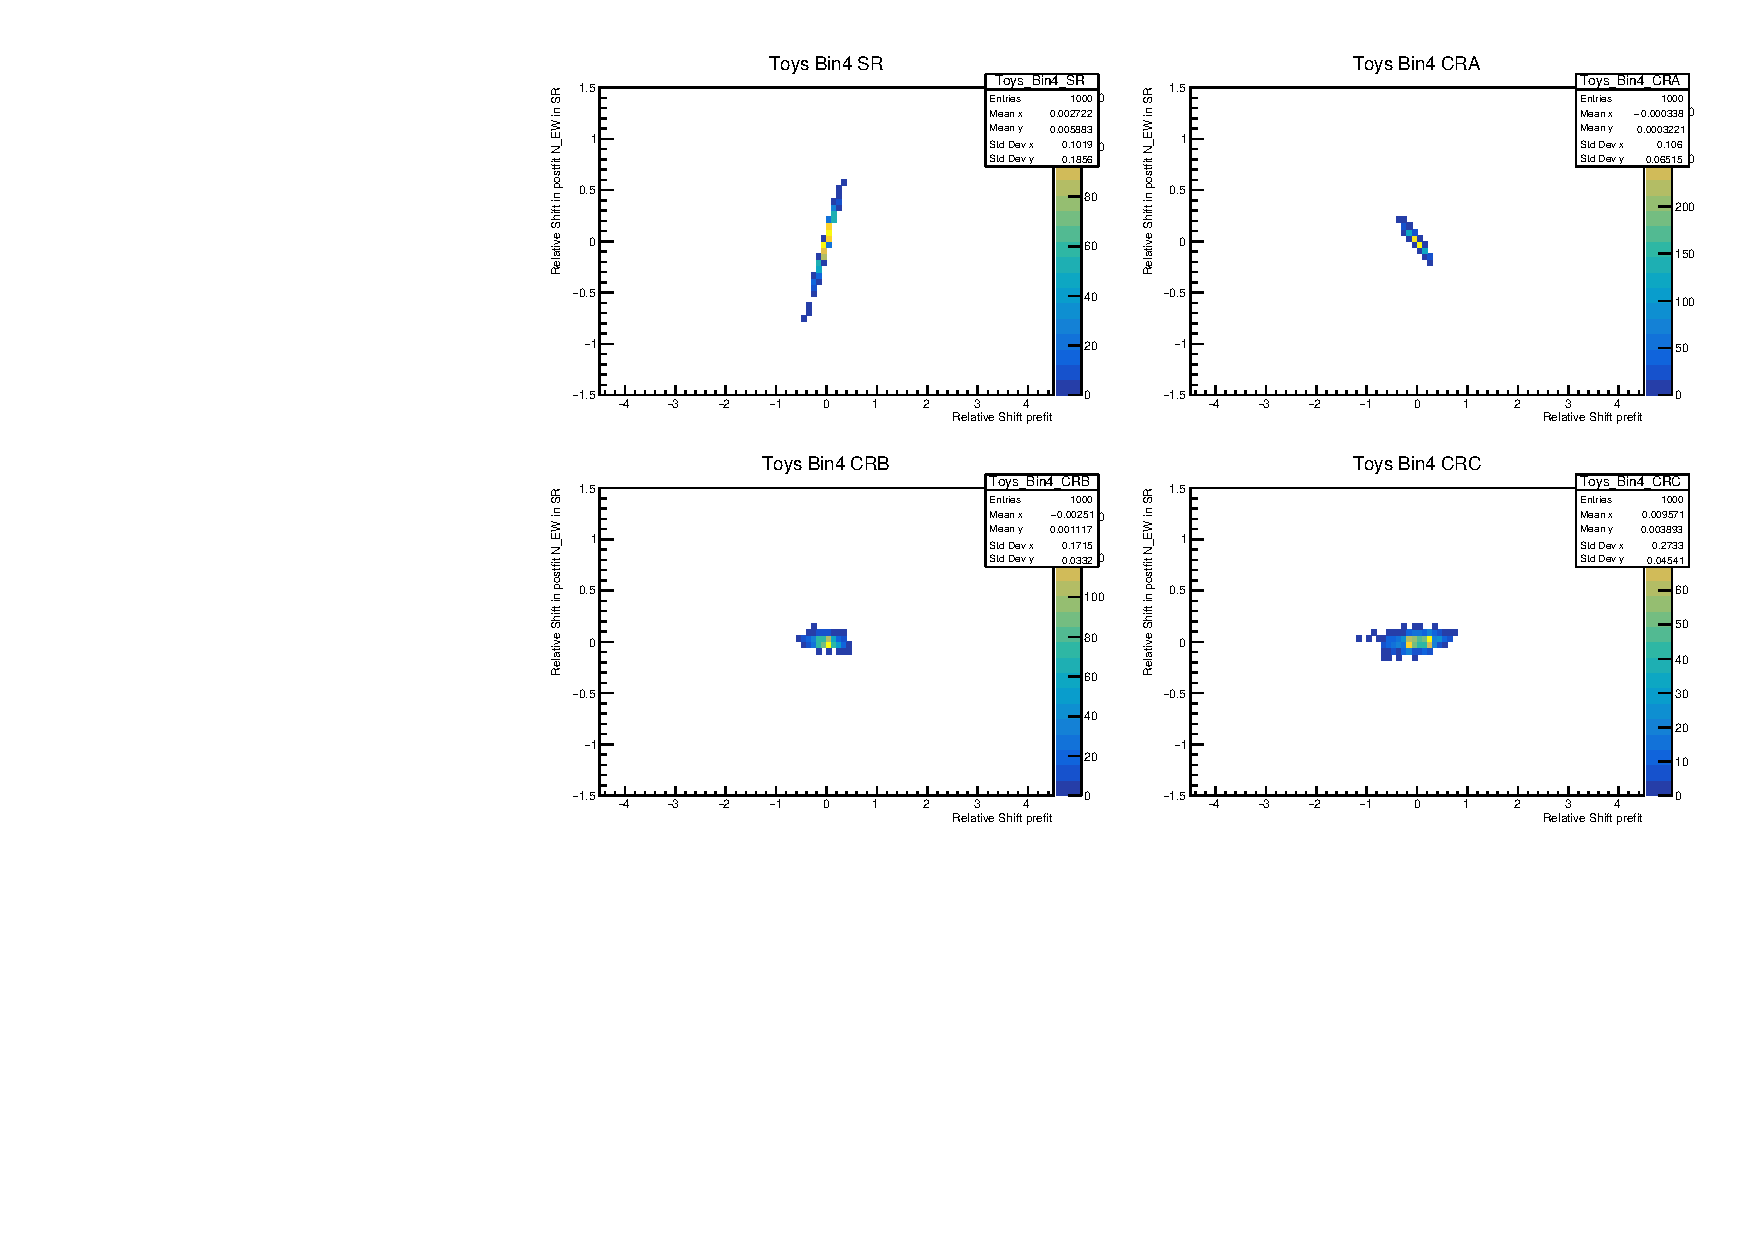
\includegraphics[width=\textwidth]{plots/diffx/instab/constfx/instabilities_mjj_QCD_Mgraph_Signal_Sh2211_BSDATASTATS_sherpaasimov_bin4.pdf}
\end{figure}

\subsubsection{\mjj QCD template fluctuations, MG5 QCD in Asimov, MG5 QCD template}
\begin{figure}[H]
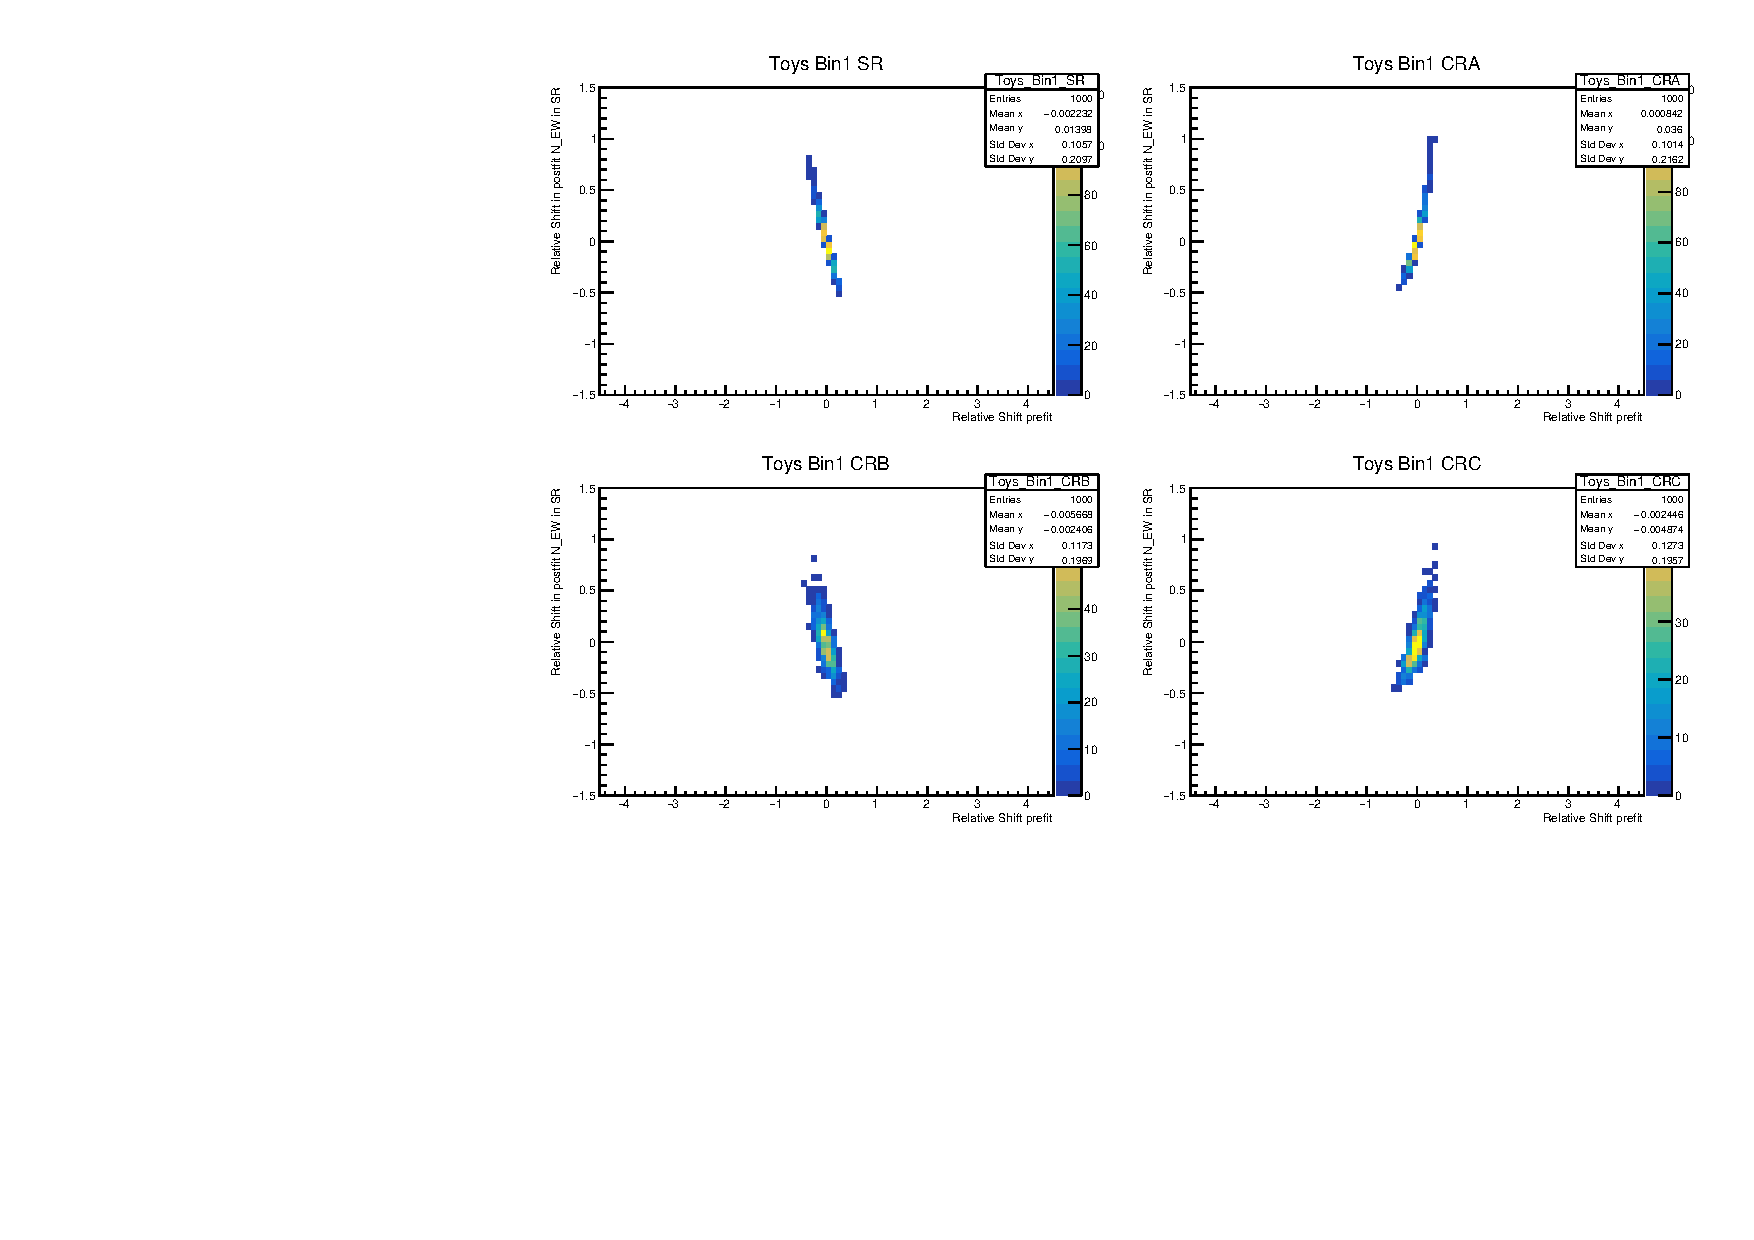
\includegraphics[width=\textwidth]{plots/diffx/instab/constfx/instabilities_mjj_QCD_Mgraph_Signal_Sh2211_BSMCQCDSTATS_madgraphasimov_bin1.pdf}
\end{figure}
\begin{figure}[H]
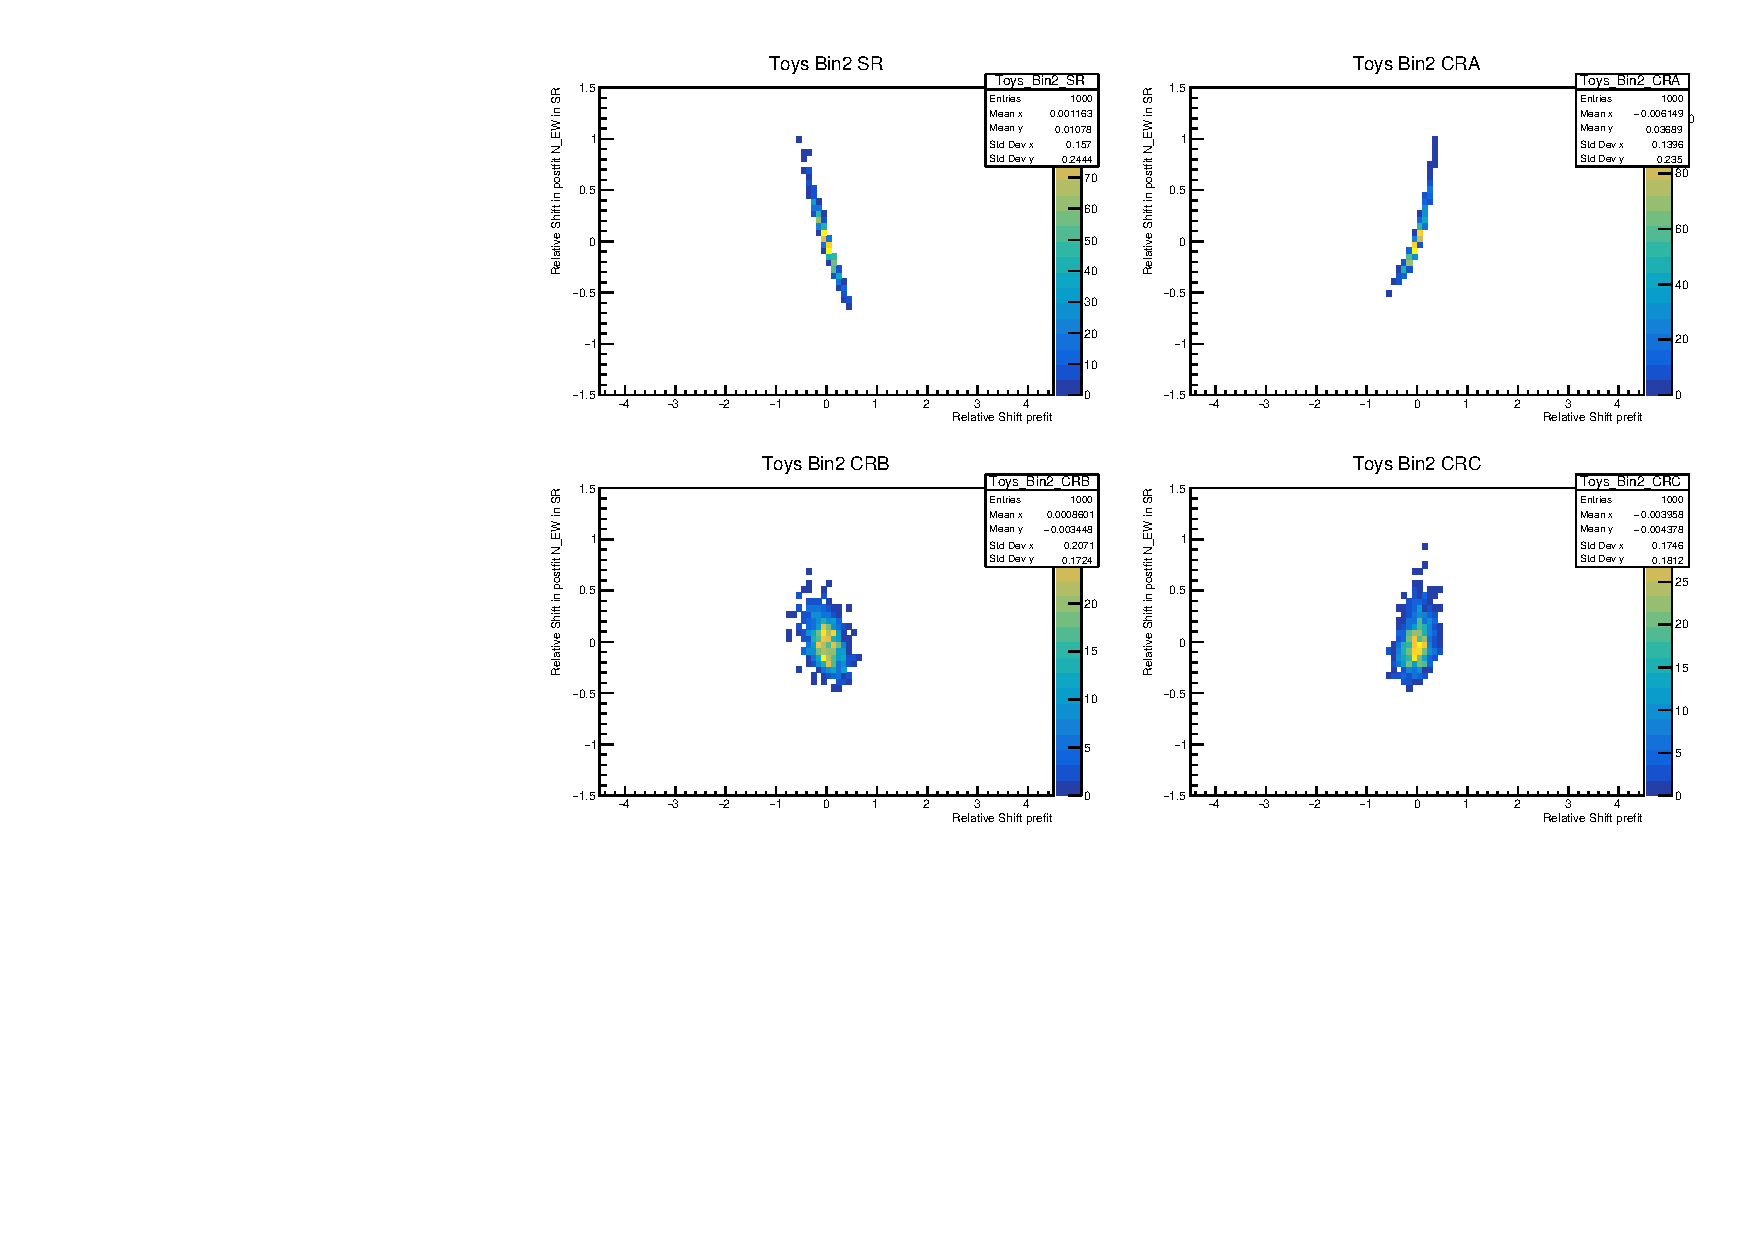
\includegraphics[width=\textwidth]{plots/diffx/instab/constfx/instabilities_mjj_QCD_Mgraph_Signal_Sh2211_BSMCQCDSTATS_madgraphasimov_bin2.pdf}
\end{figure}
\begin{figure}[H]
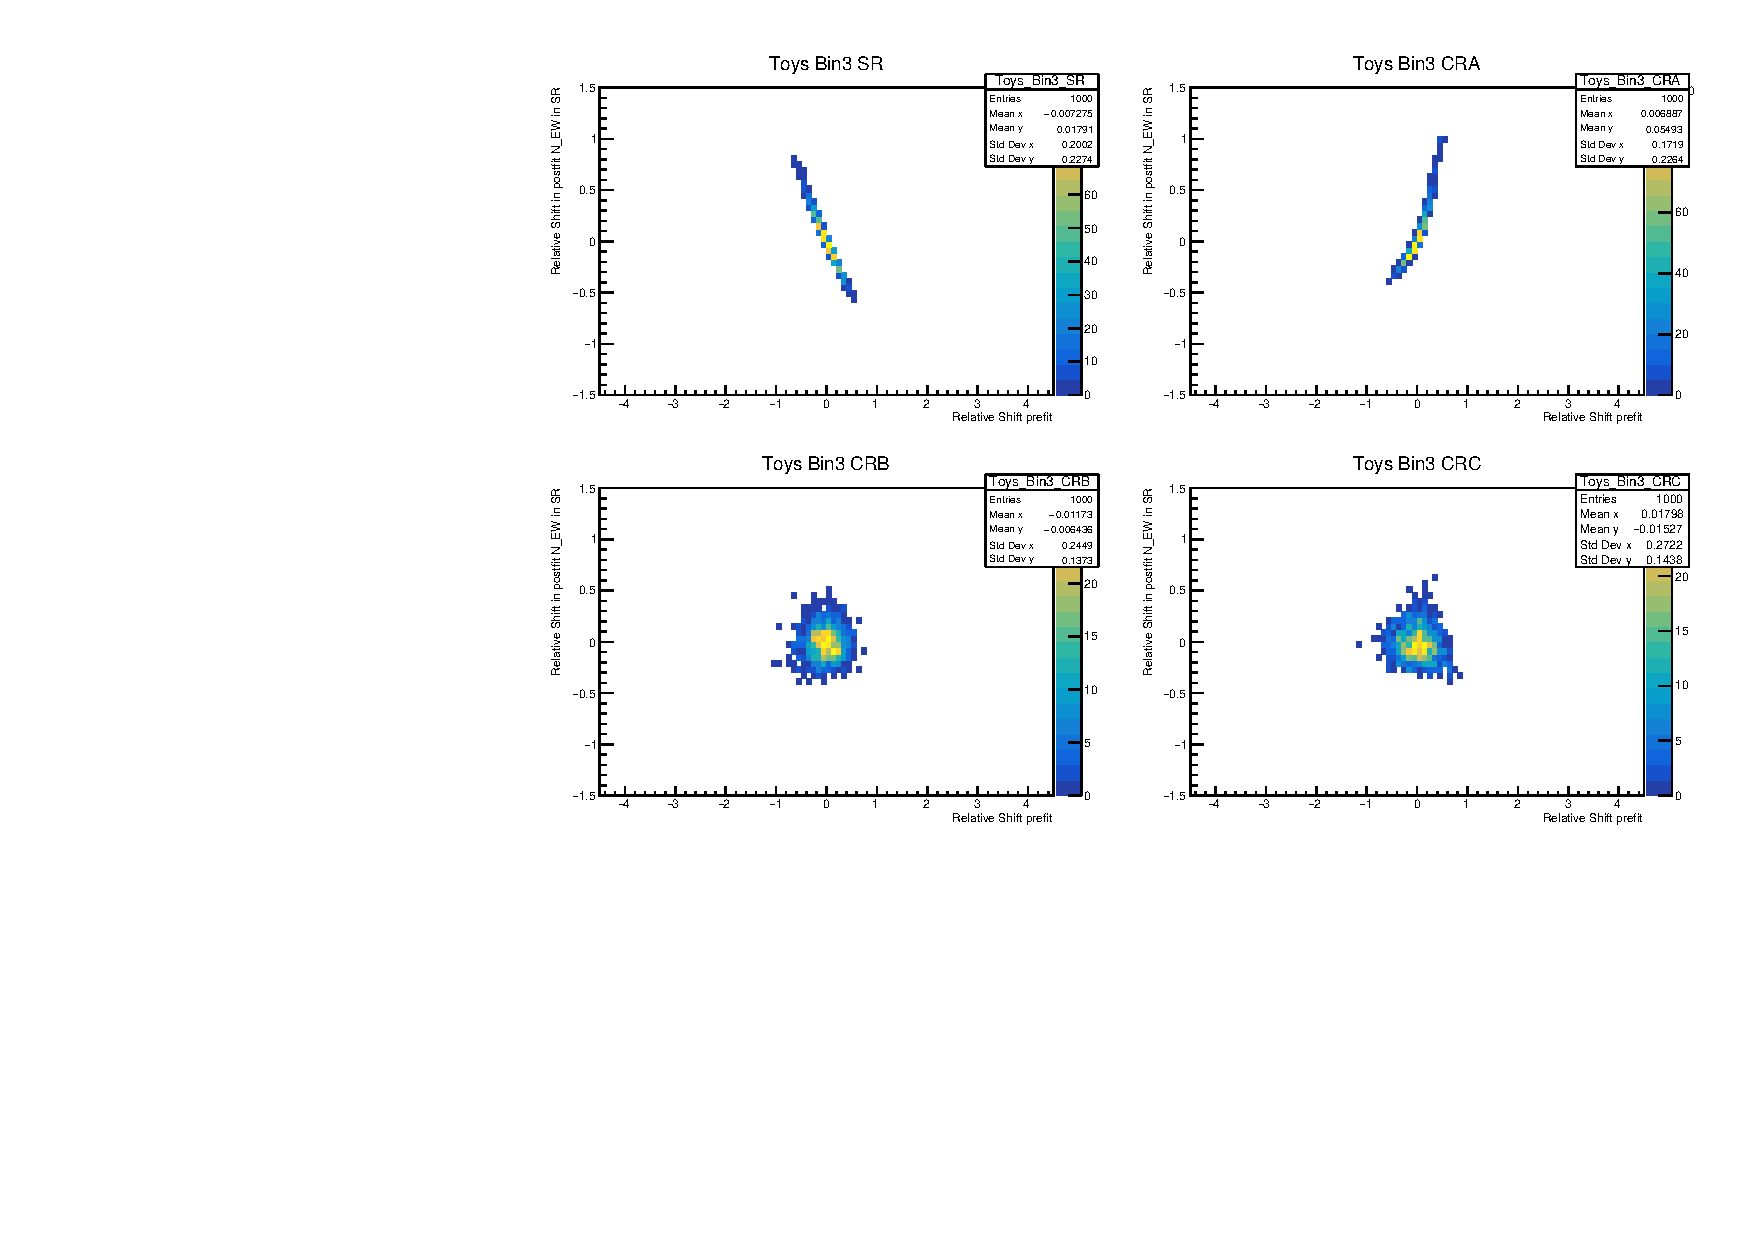
\includegraphics[width=\textwidth]{plots/diffx/instab/constfx/instabilities_mjj_QCD_Mgraph_Signal_Sh2211_BSMCQCDSTATS_madgraphasimov_bin3.pdf}
\end{figure}
\begin{figure}[H]
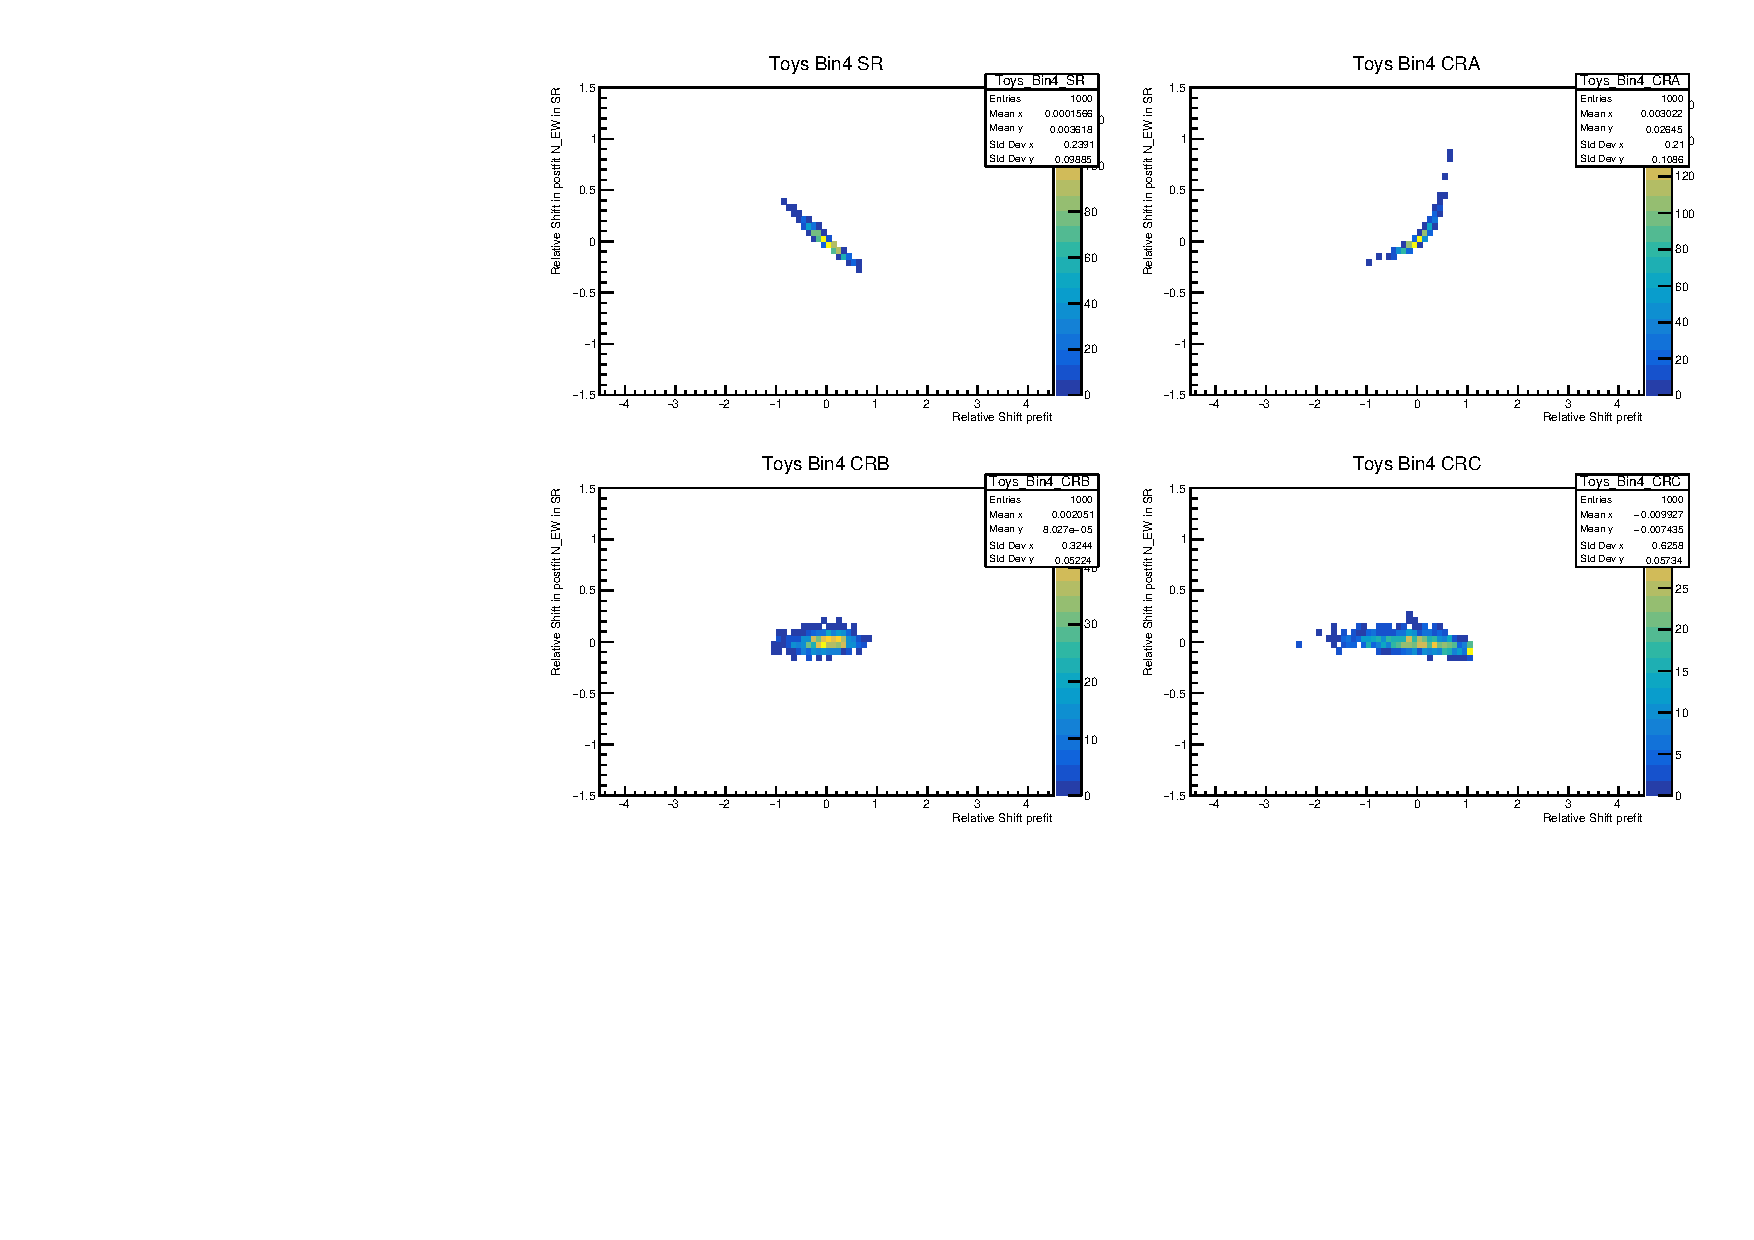
\includegraphics[width=\textwidth]{plots/diffx/instab/constfx/instabilities_mjj_QCD_Mgraph_Signal_Sh2211_BSMCQCDSTATS_madgraphasimov_bin4.pdf}
\end{figure}

\subsubsection{\mjj QCD template fluctuations, Sherpa-2.2.11 QCD in Asimov, MG5 QCD template}
\begin{figure}[H]
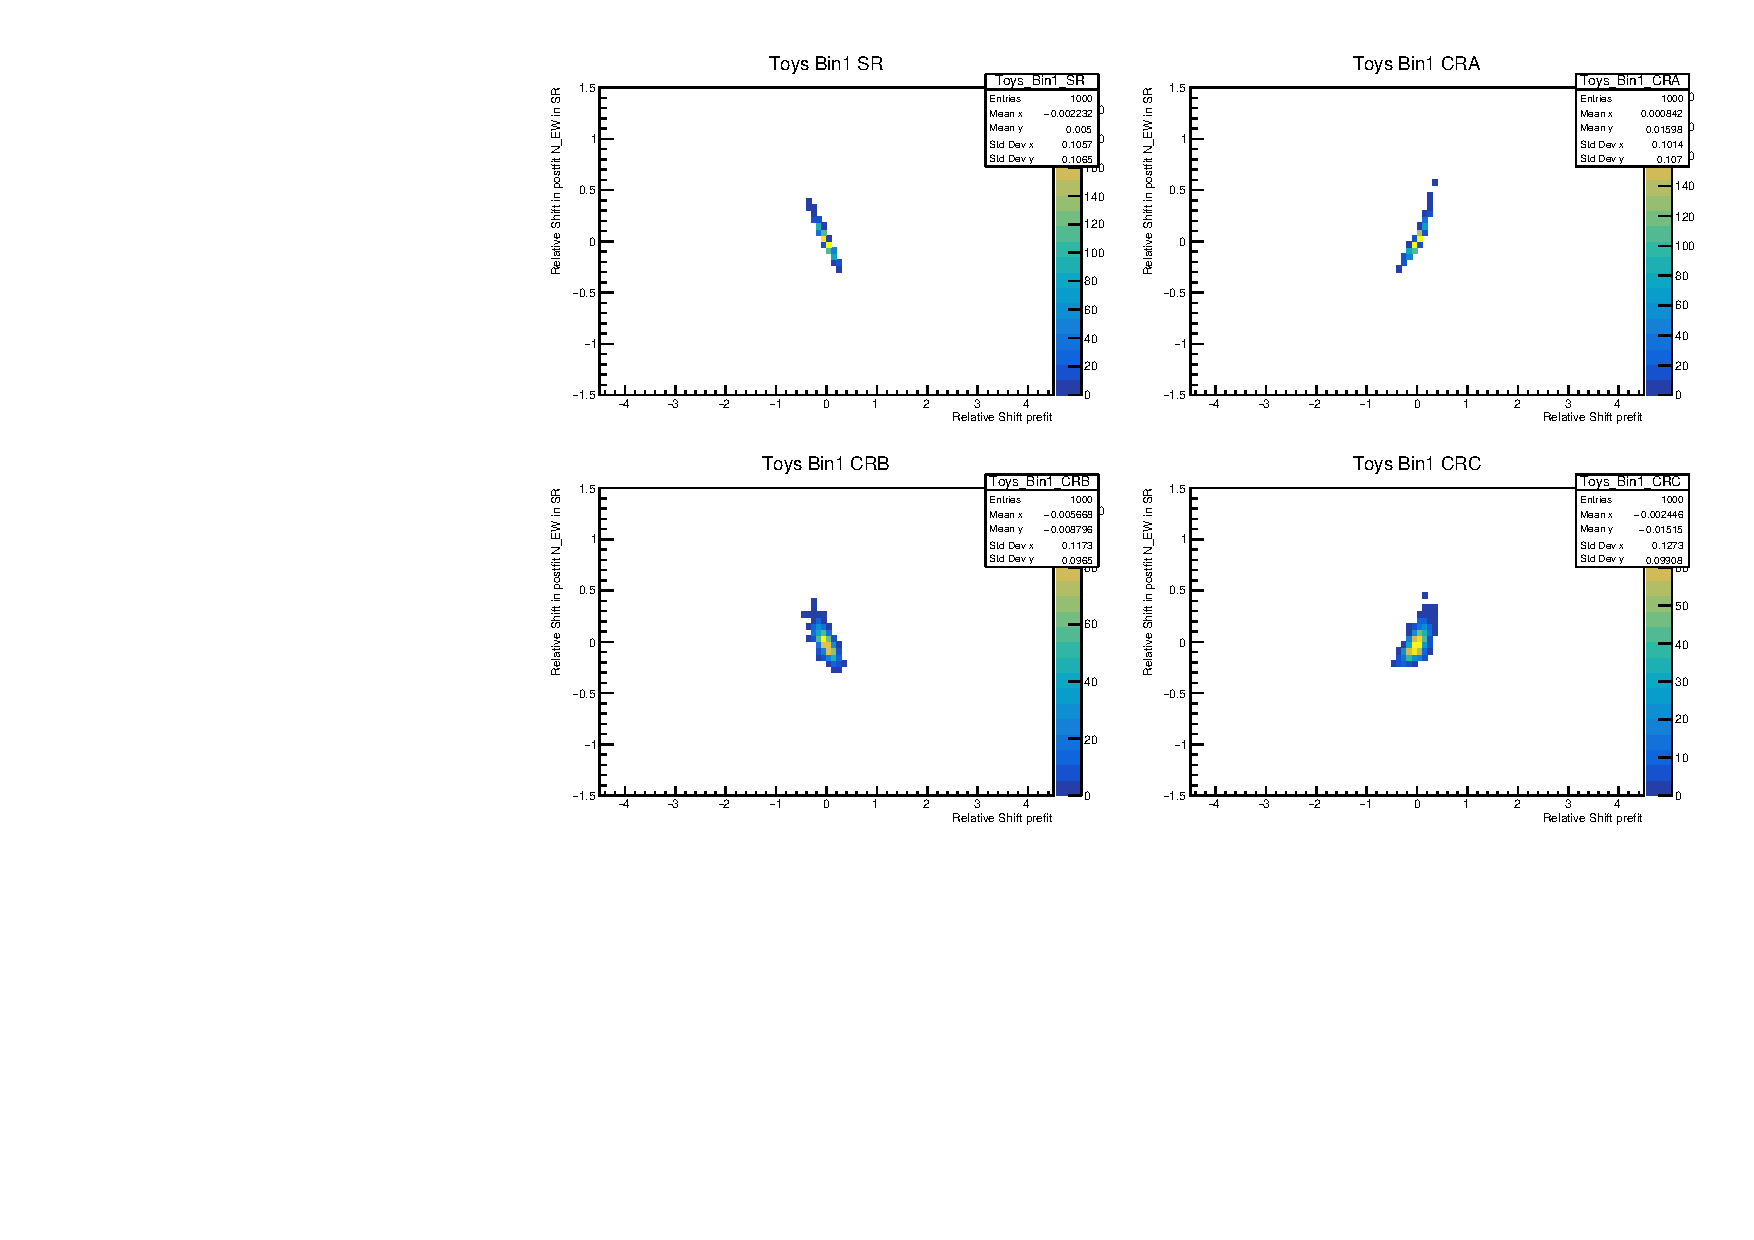
\includegraphics[width=\textwidth]{plots/diffx/instab/constfx/instabilities_mjj_QCD_Mgraph_Signal_Sh2211_BSMCQCDSTATS_sherpaasimov_bin1.pdf}
\end{figure}
\begin{figure}[H]
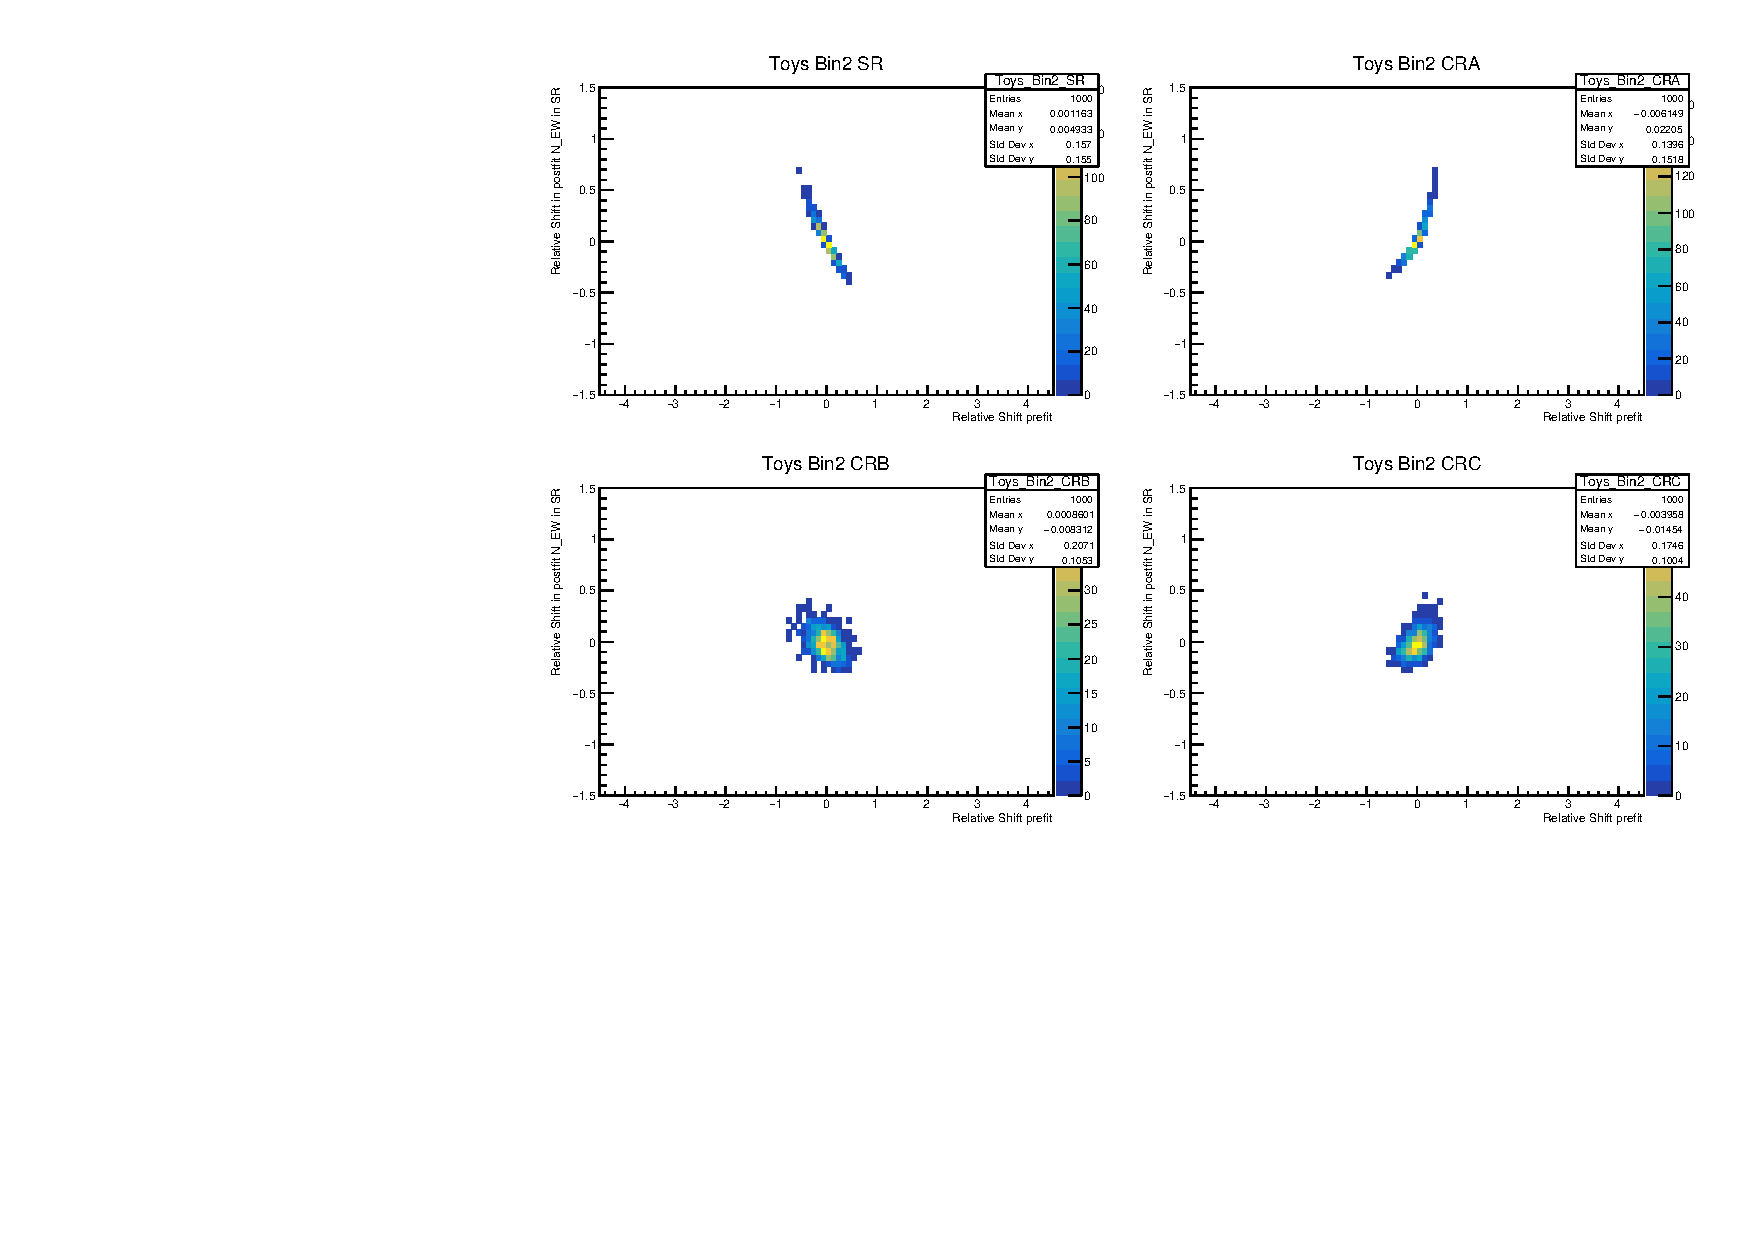
\includegraphics[width=\textwidth]{plots/diffx/instab/constfx/instabilities_mjj_QCD_Mgraph_Signal_Sh2211_BSMCQCDSTATS_sherpaasimov_bin2.pdf}
\end{figure}
\begin{figure}[H]
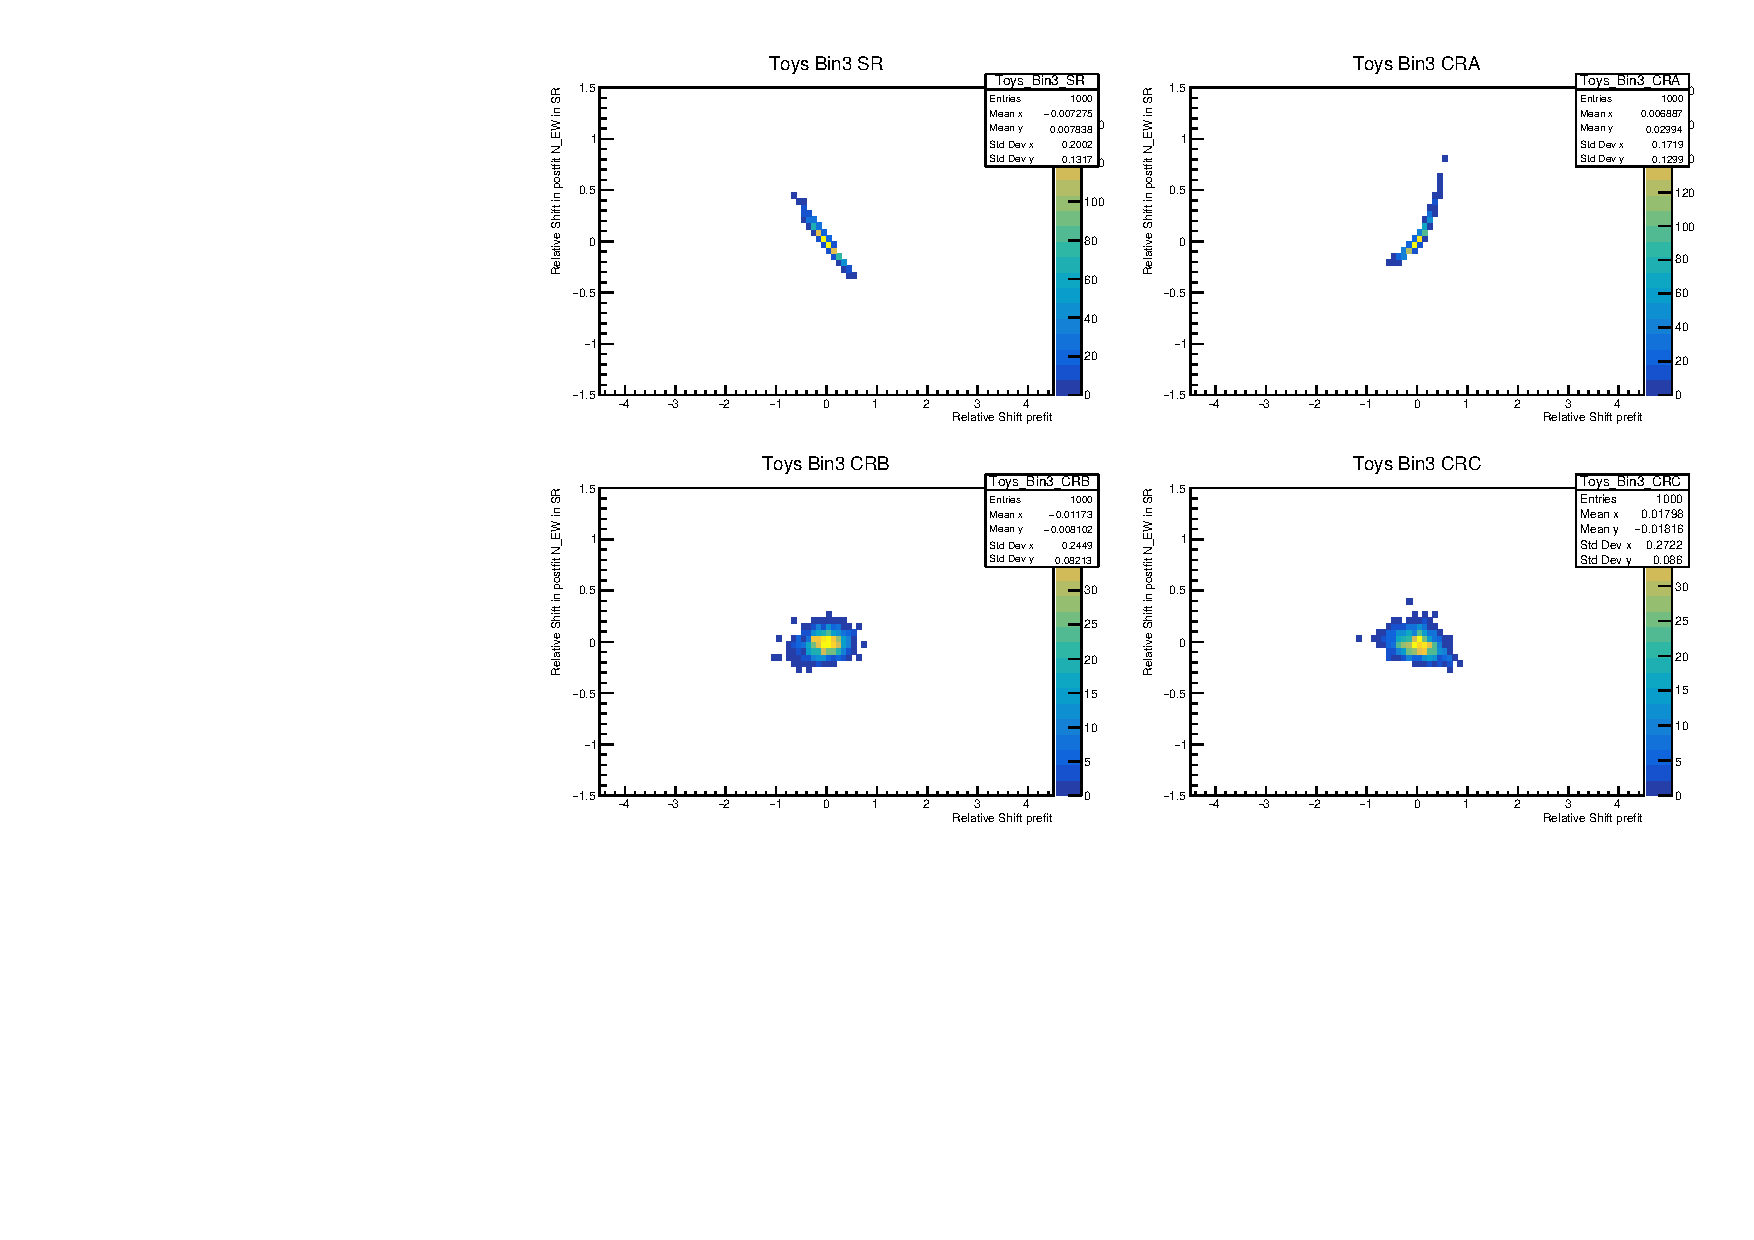
\includegraphics[width=\textwidth]{plots/diffx/instab/constfx/instabilities_mjj_QCD_Mgraph_Signal_Sh2211_BSMCQCDSTATS_sherpaasimov_bin3.pdf}
\end{figure}
\begin{figure}[H]
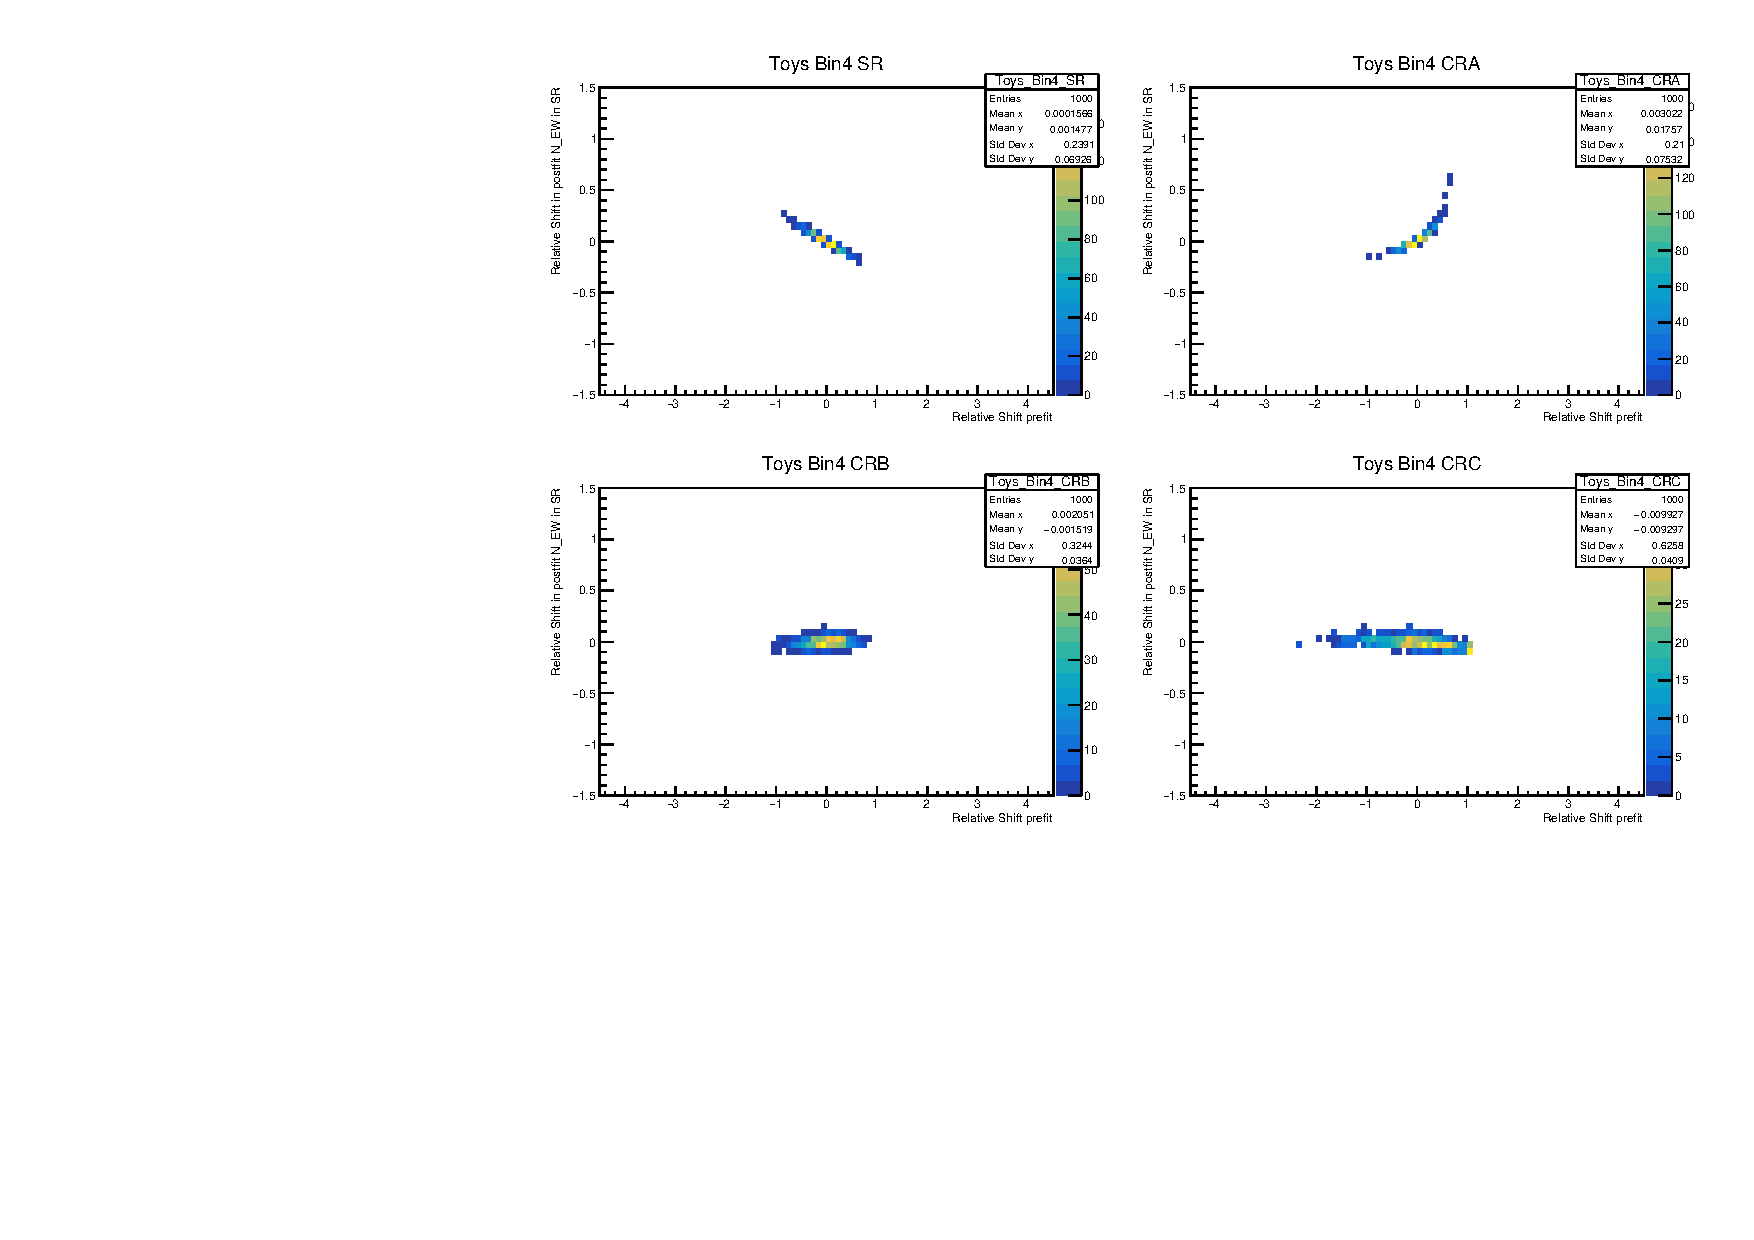
\includegraphics[width=\textwidth]{plots/diffx/instab/constfx/instabilities_mjj_QCD_Mgraph_Signal_Sh2211_BSMCQCDSTATS_sherpaasimov_bin4.pdf}
\end{figure}

\subsubsection{\mjj Asimov fluctuations, MG5 QCD in Asimov, Sherpa-2.2.11 QCD template}
\begin{figure}[H]
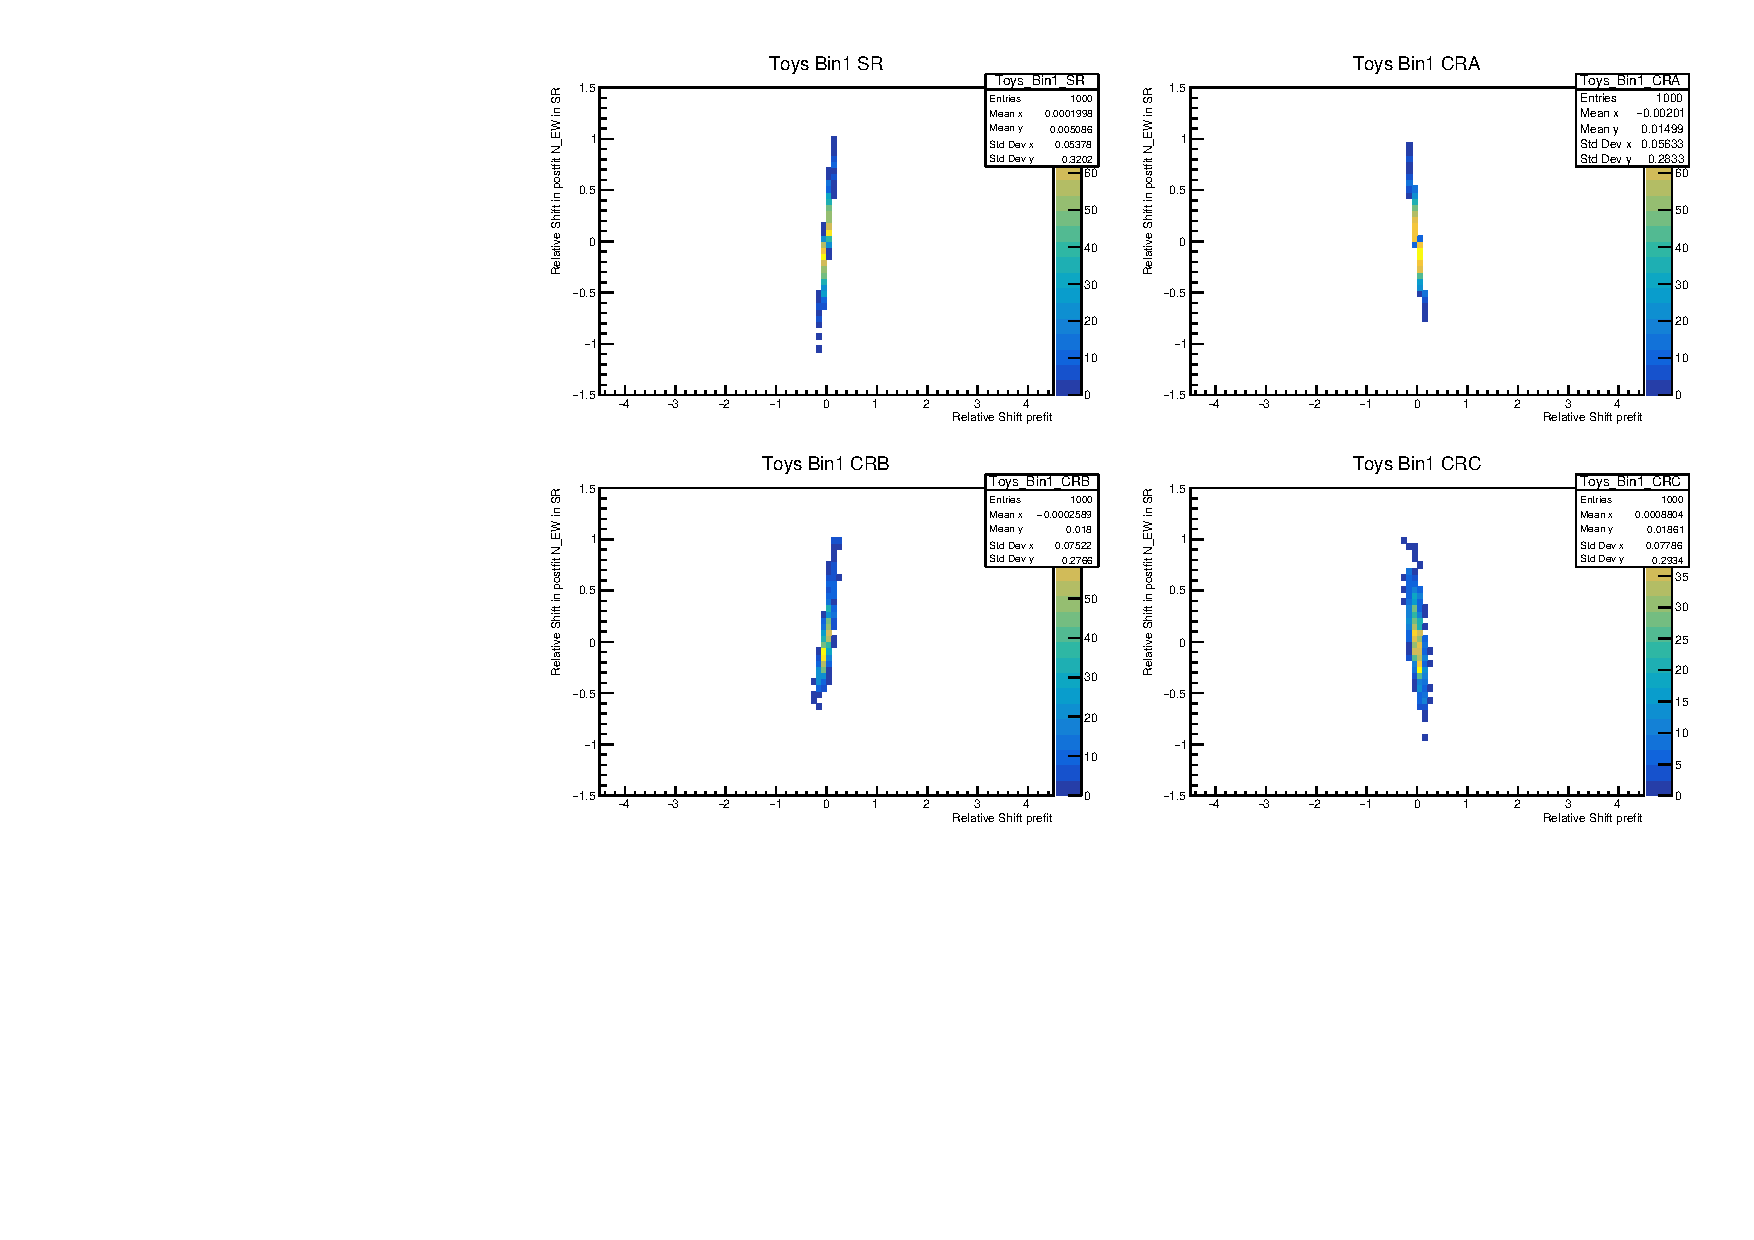
\includegraphics[width=\textwidth]{plots/diffx/instab/constfx/instabilities_mjj_QCD_Sh2211_Signal_Sh2211_BSDATASTATS_madgraphasimov_bin1.pdf}
\end{figure}
\begin{figure}[H]
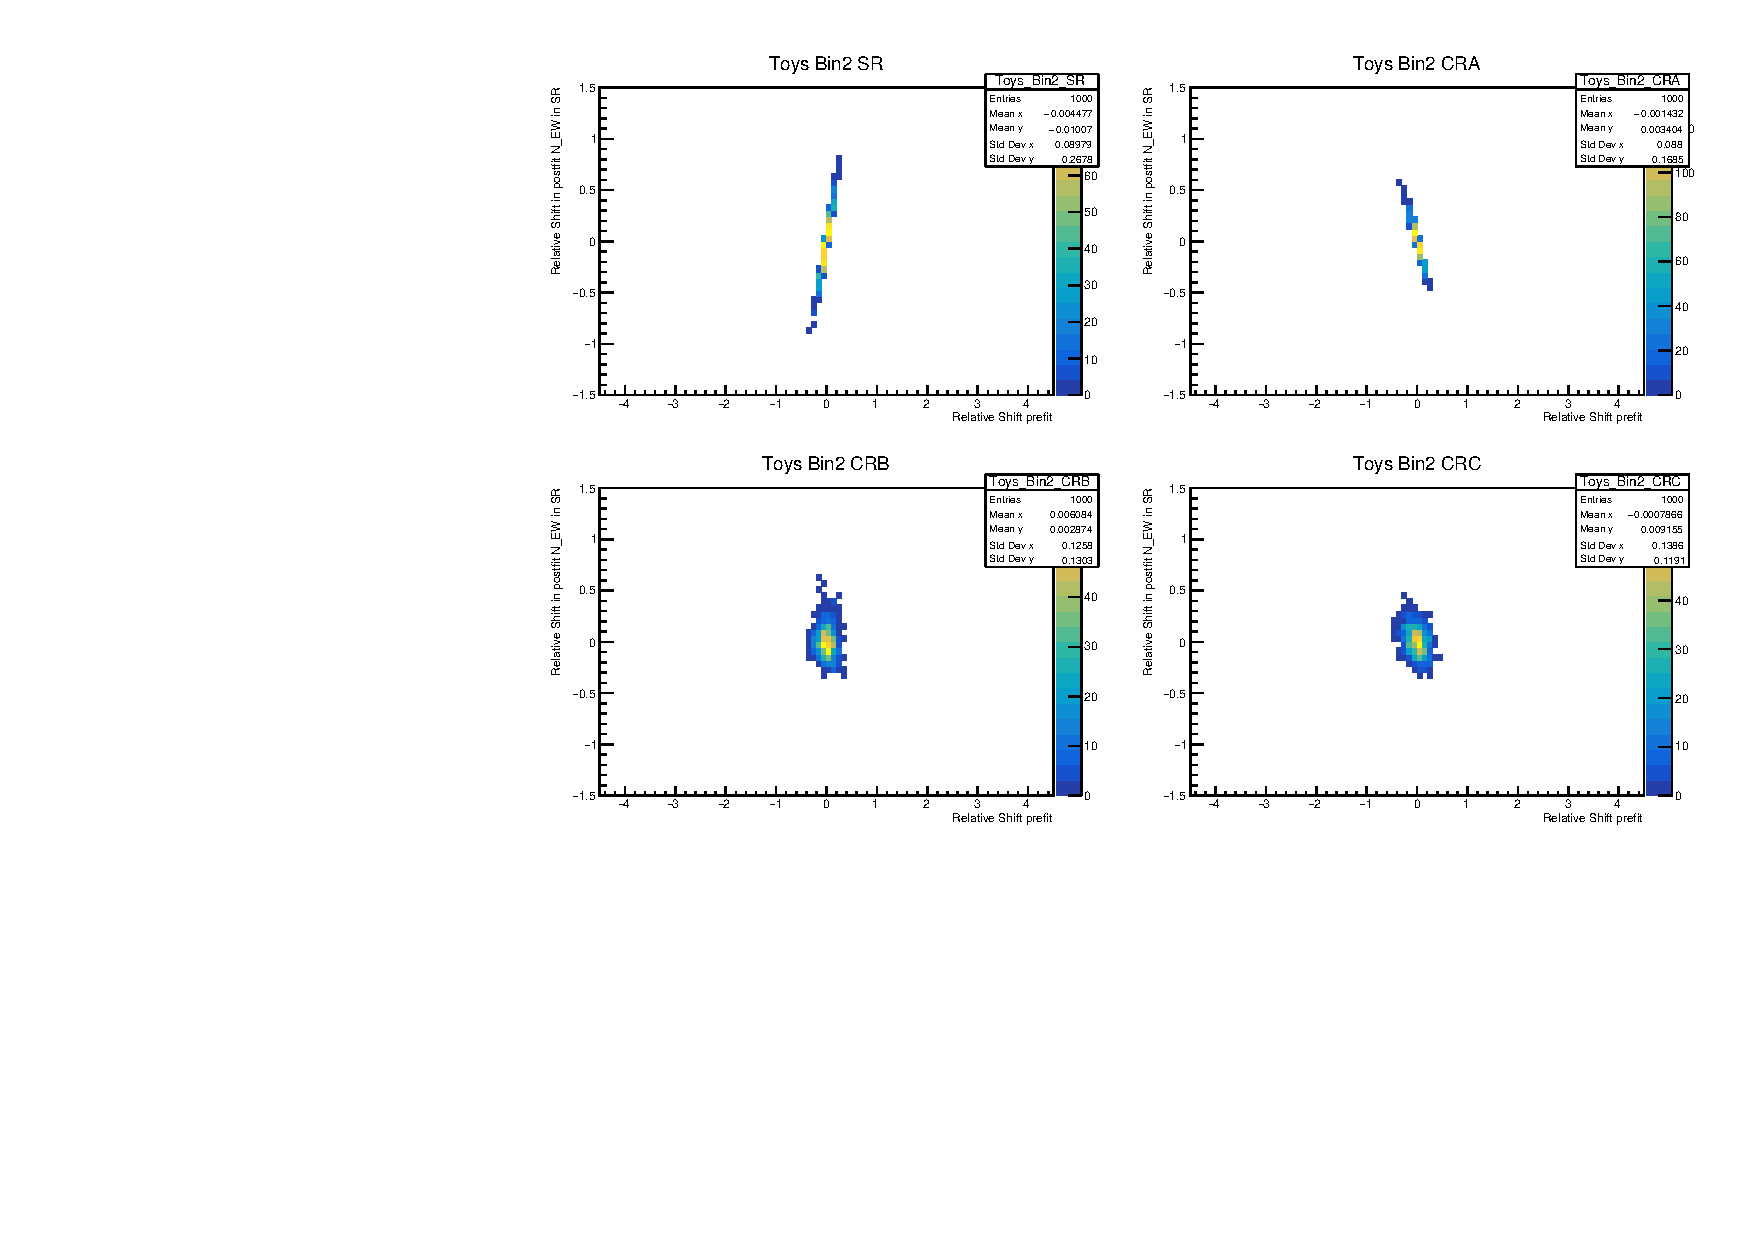
\includegraphics[width=\textwidth]{plots/diffx/instab/constfx/instabilities_mjj_QCD_Sh2211_Signal_Sh2211_BSDATASTATS_madgraphasimov_bin2.pdf}
\end{figure}
\begin{figure}[H]
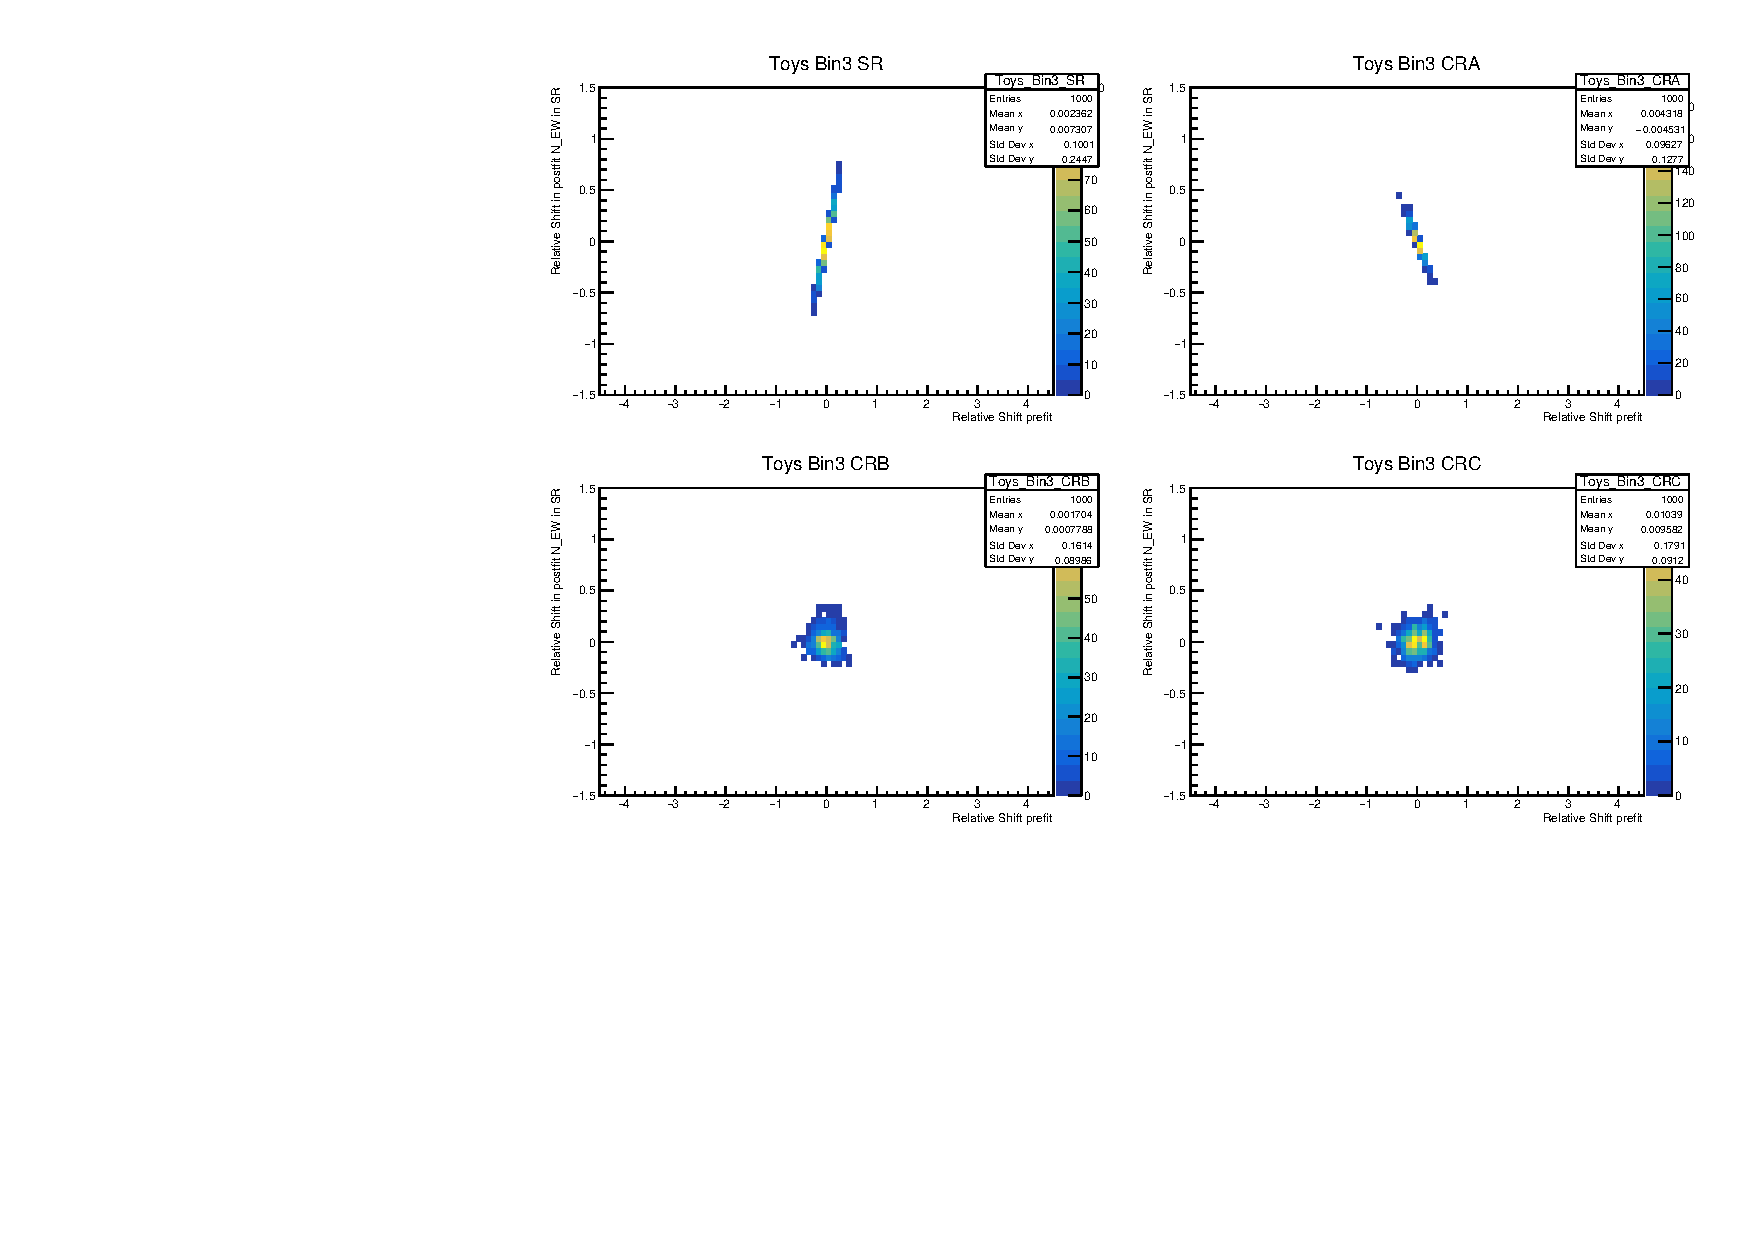
\includegraphics[width=\textwidth]{plots/diffx/instab/constfx/instabilities_mjj_QCD_Sh2211_Signal_Sh2211_BSDATASTATS_madgraphasimov_bin3.pdf}
\end{figure}
\begin{figure}[H]
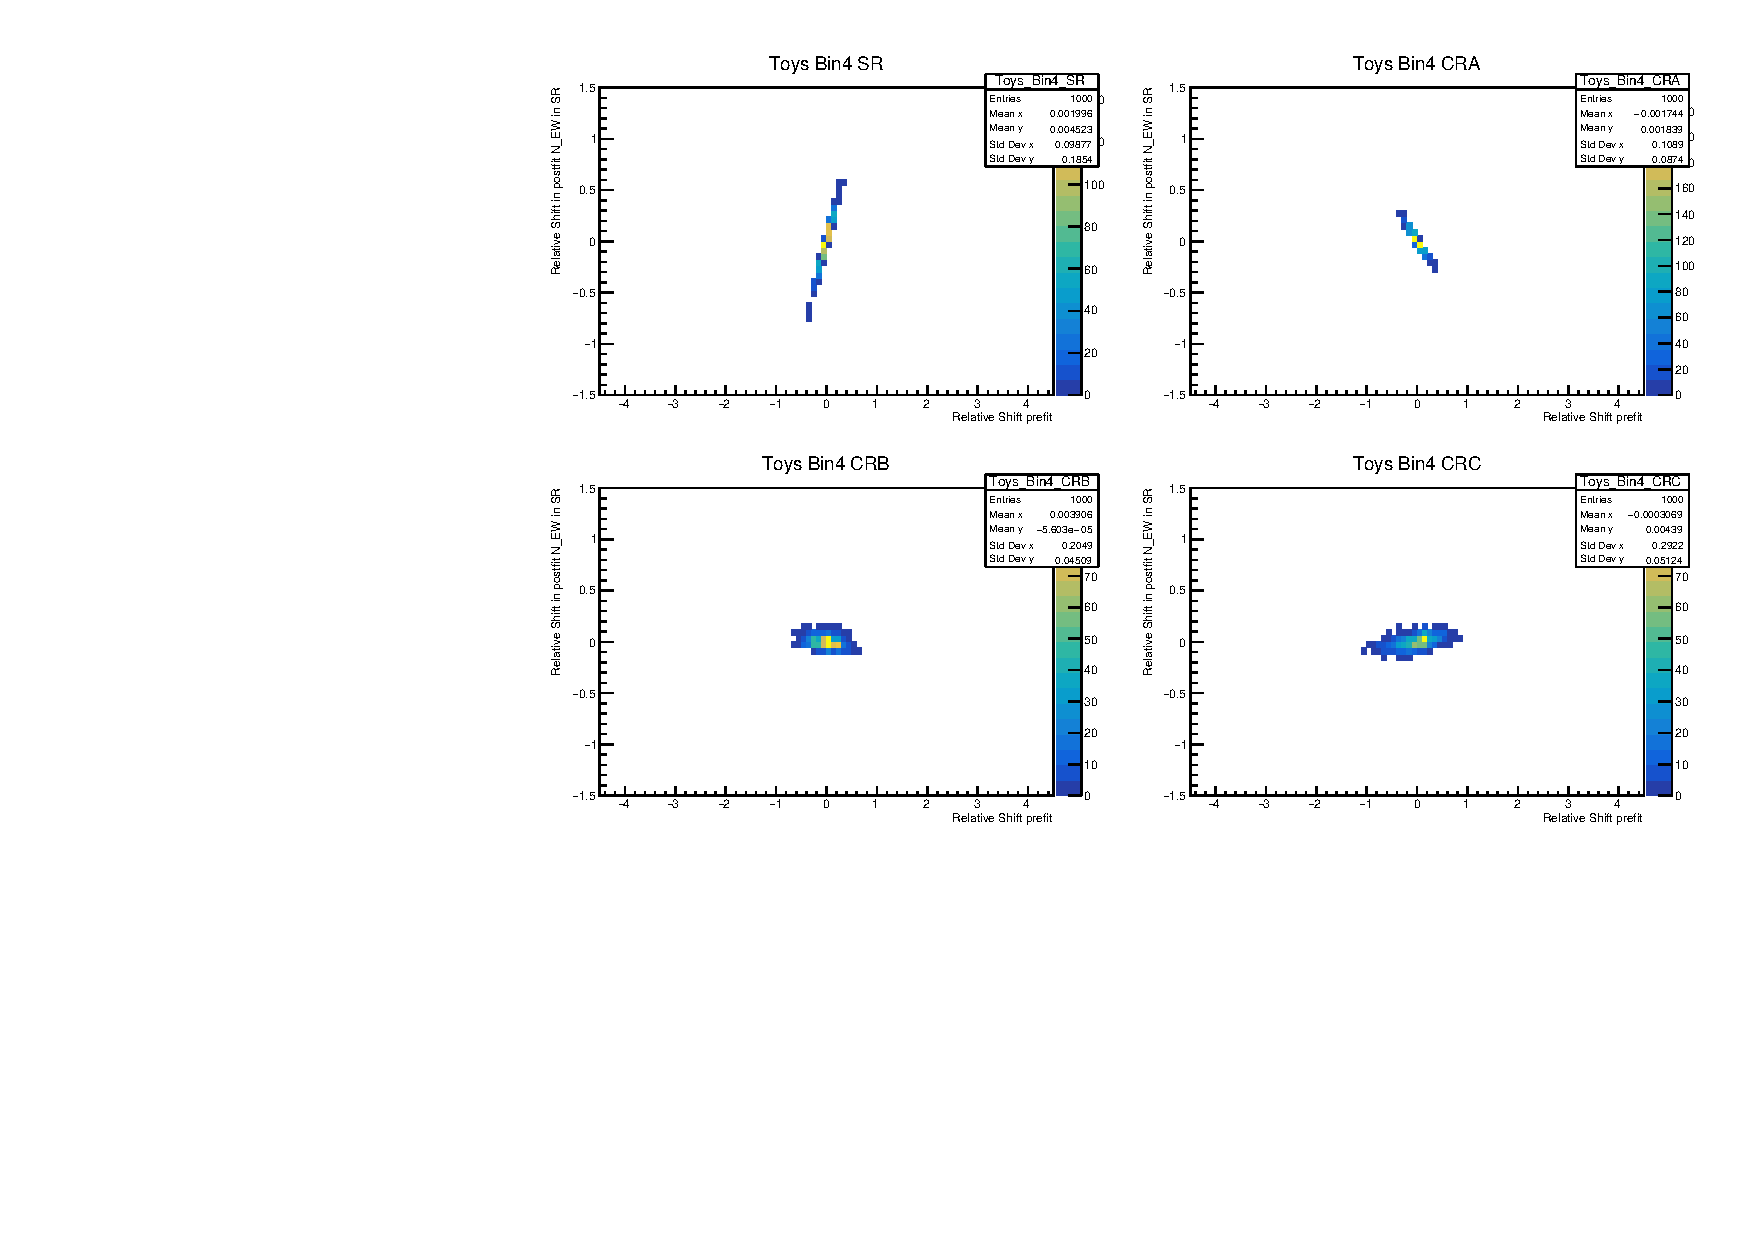
\includegraphics[width=\textwidth]{plots/diffx/instab/constfx/instabilities_mjj_QCD_Sh2211_Signal_Sh2211_BSDATASTATS_madgraphasimov_bin4.pdf}
\end{figure}

\subsubsection{\mjj Asimov fluctuations, Sherpa-2.2.11 QCD in Asimov, Sherpa-2.2.11 QCD template}
\begin{figure}[H]
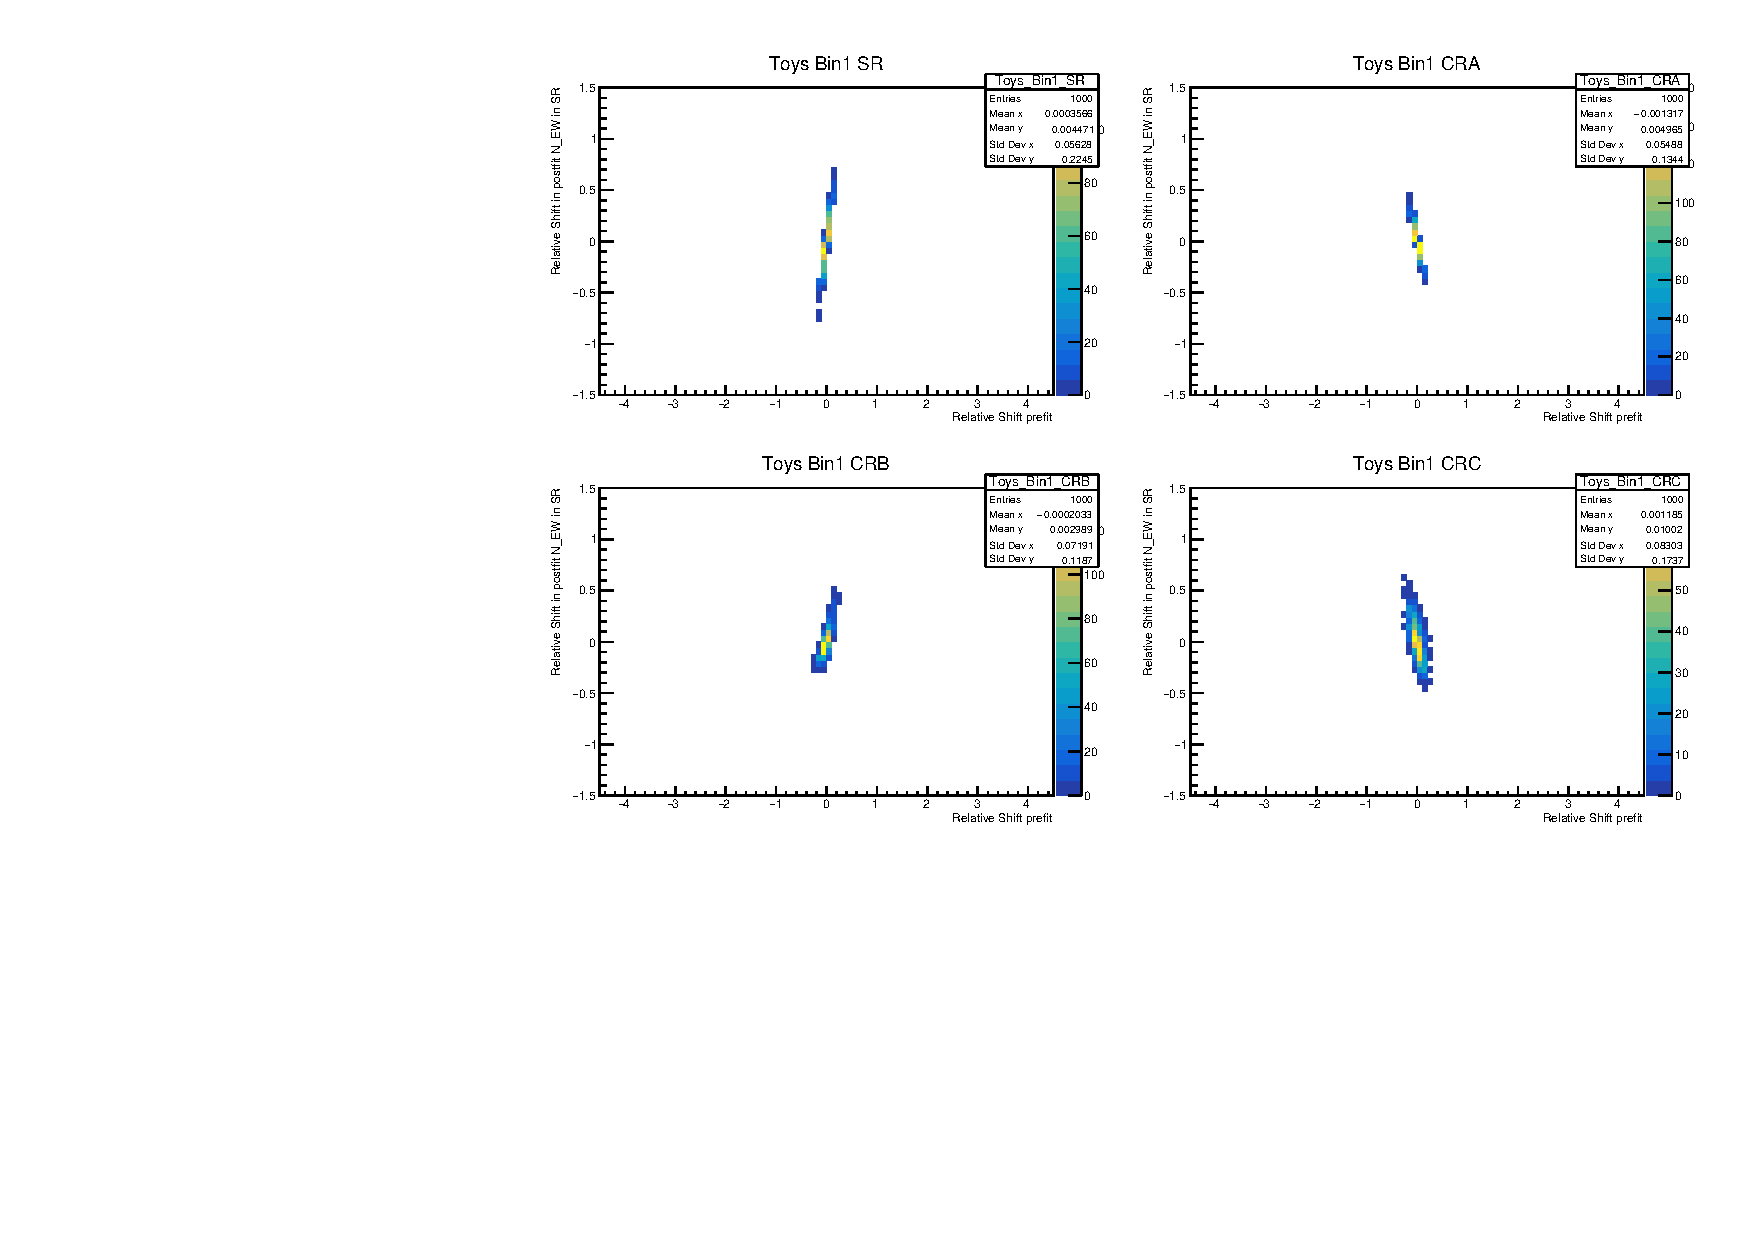
\includegraphics[width=\textwidth]{plots/diffx/instab/constfx/instabilities_mjj_QCD_Sh2211_Signal_Sh2211_BSDATASTATS_sherpaasimov_bin1.pdf}
\end{figure}
\begin{figure}[H]
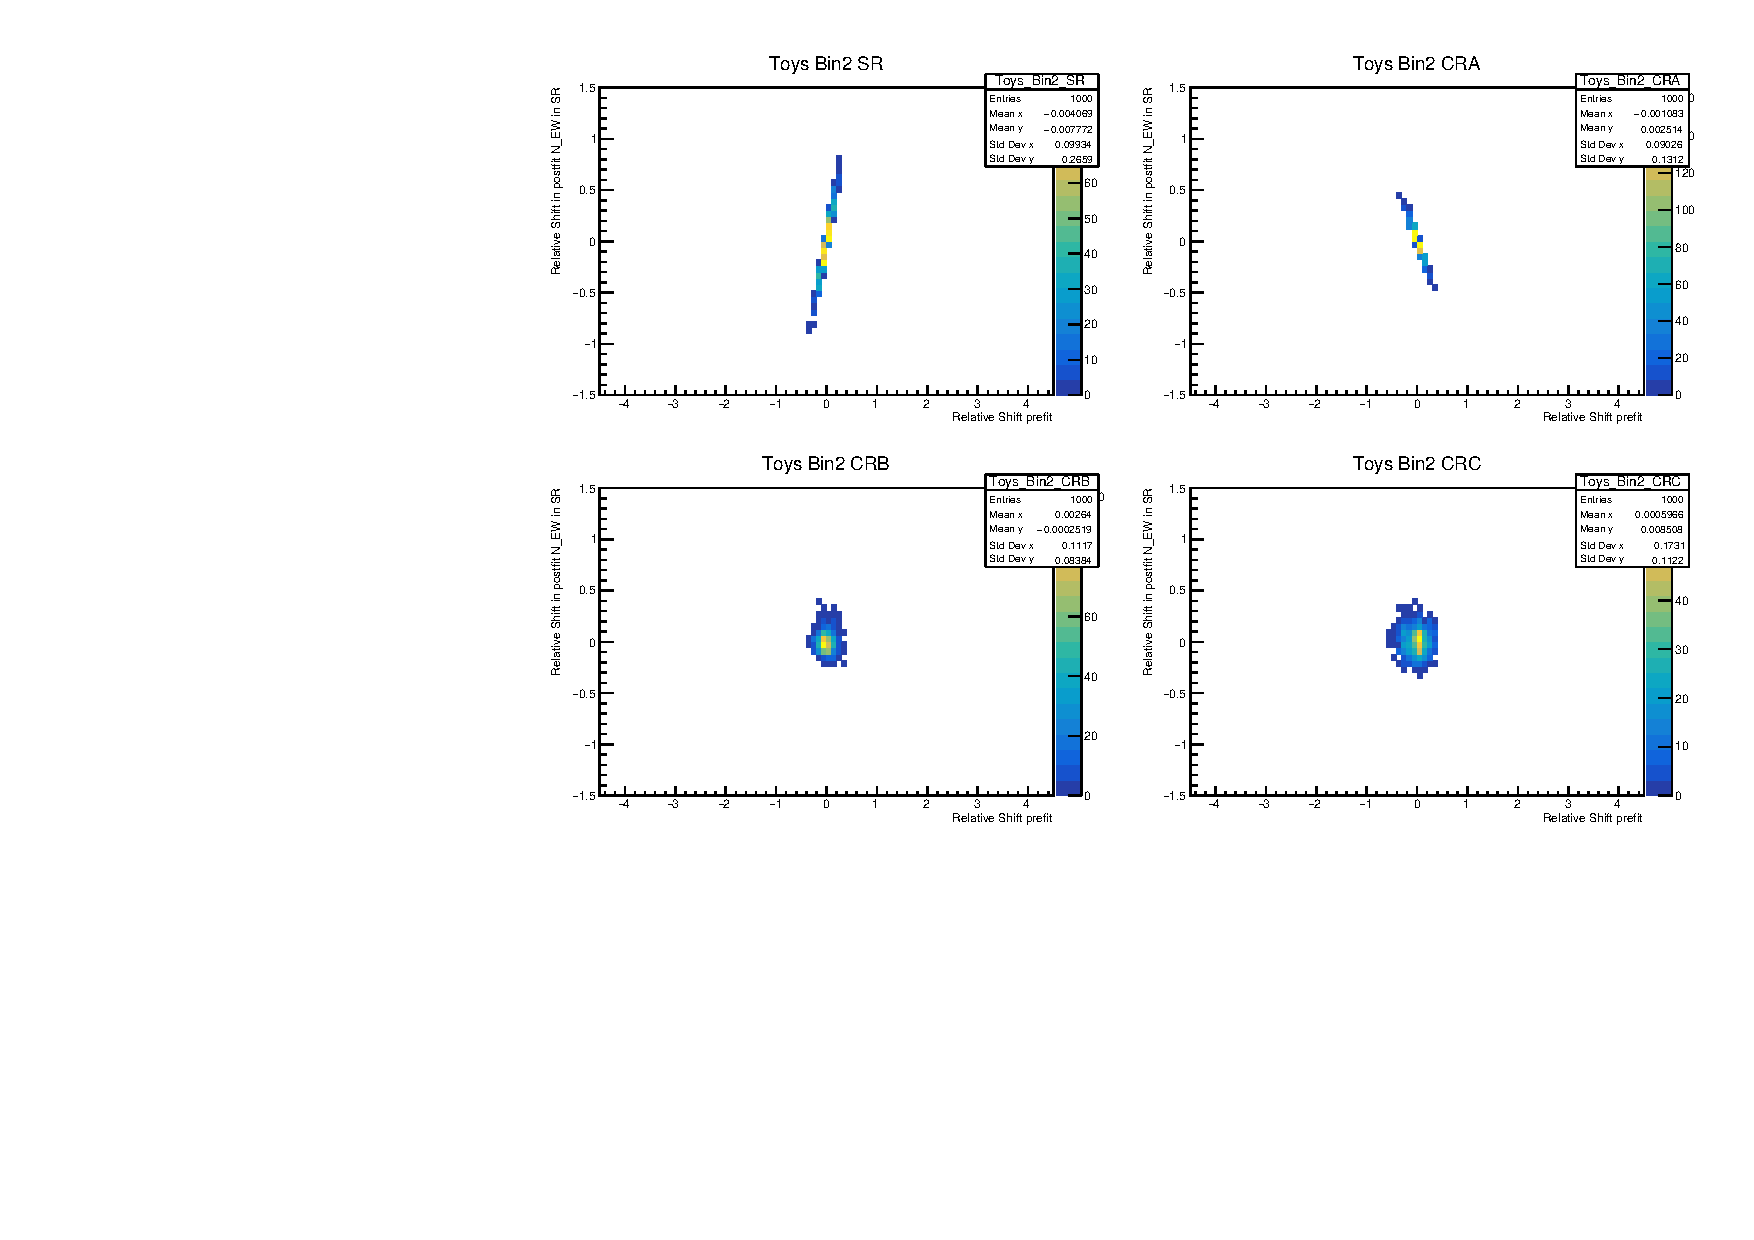
\includegraphics[width=\textwidth]{plots/diffx/instab/constfx/instabilities_mjj_QCD_Sh2211_Signal_Sh2211_BSDATASTATS_sherpaasimov_bin2.pdf}
\end{figure}
\begin{figure}[H]
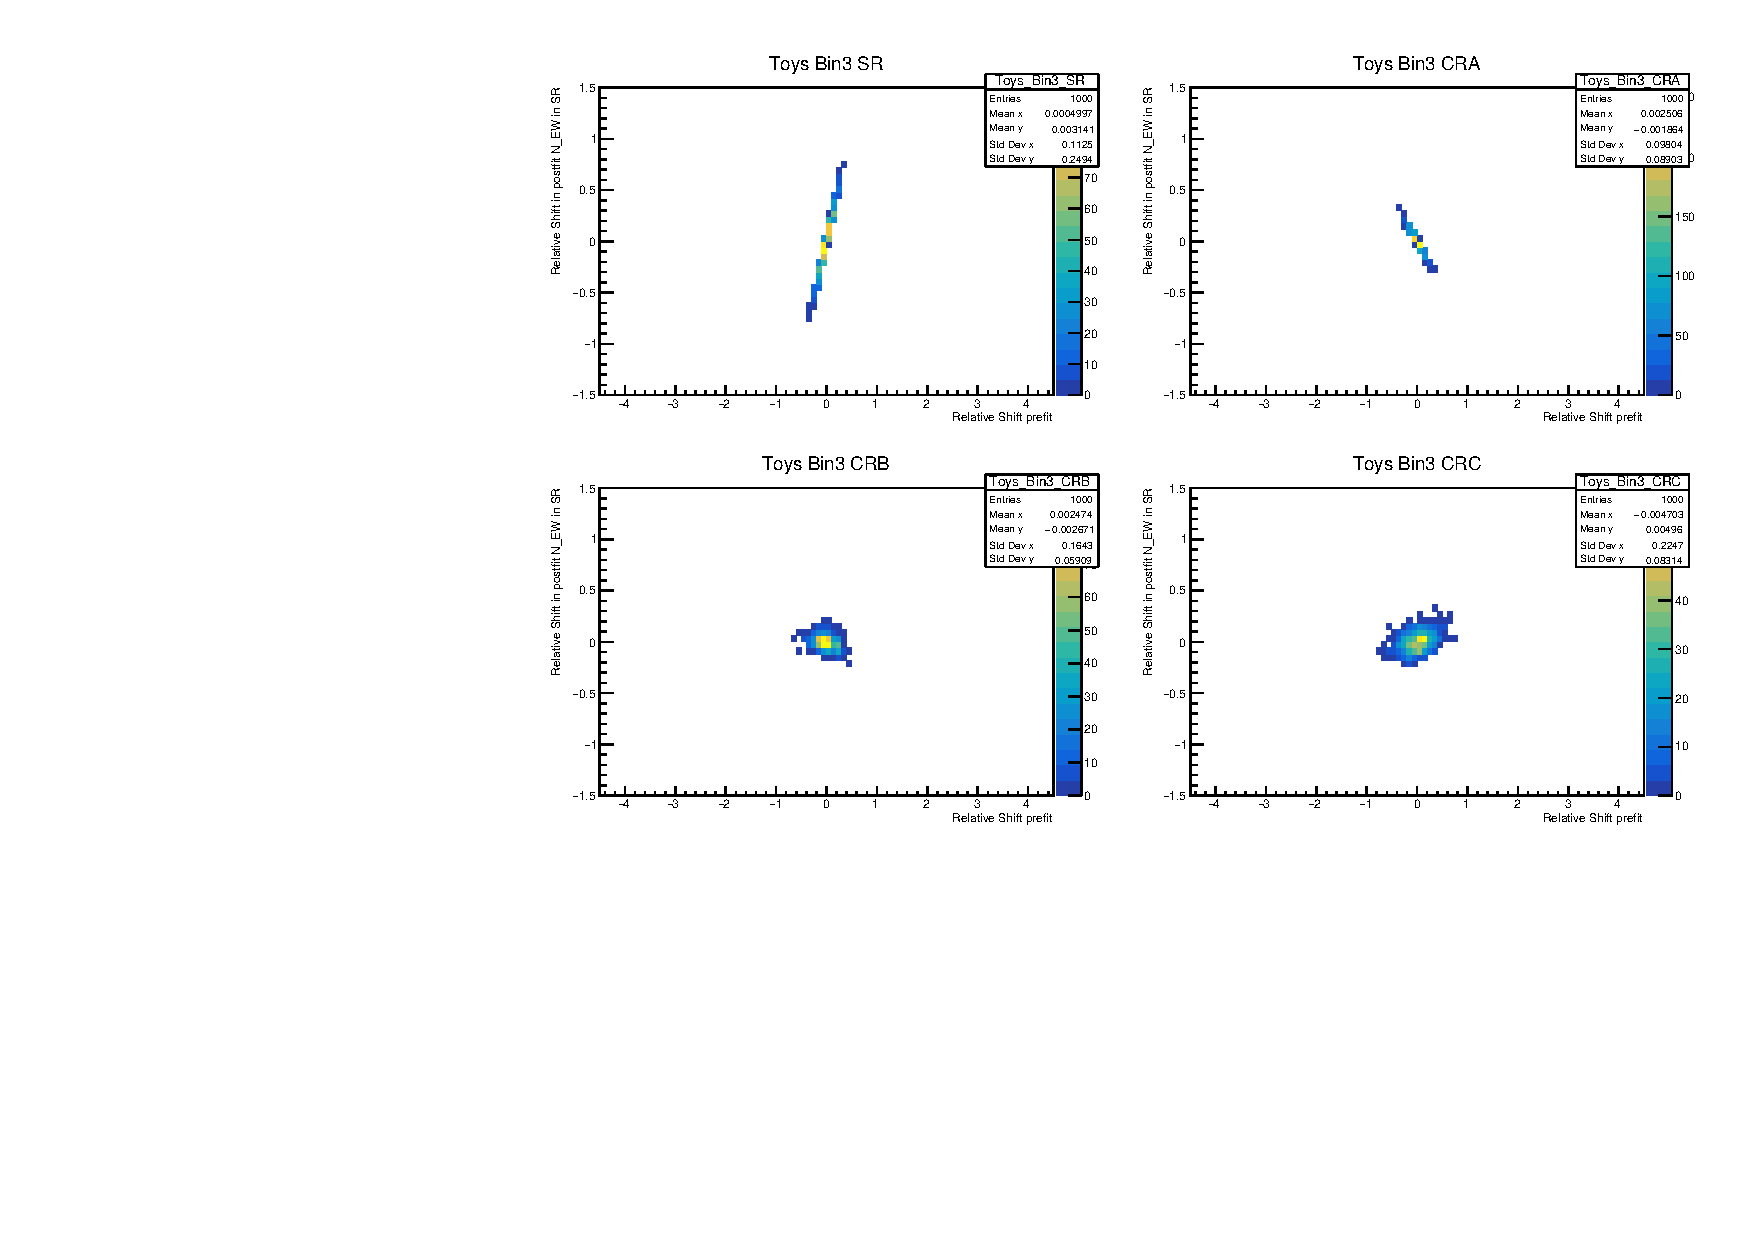
\includegraphics[width=\textwidth]{plots/diffx/instab/constfx/instabilities_mjj_QCD_Sh2211_Signal_Sh2211_BSDATASTATS_sherpaasimov_bin3.pdf}
\end{figure}
\begin{figure}[H]
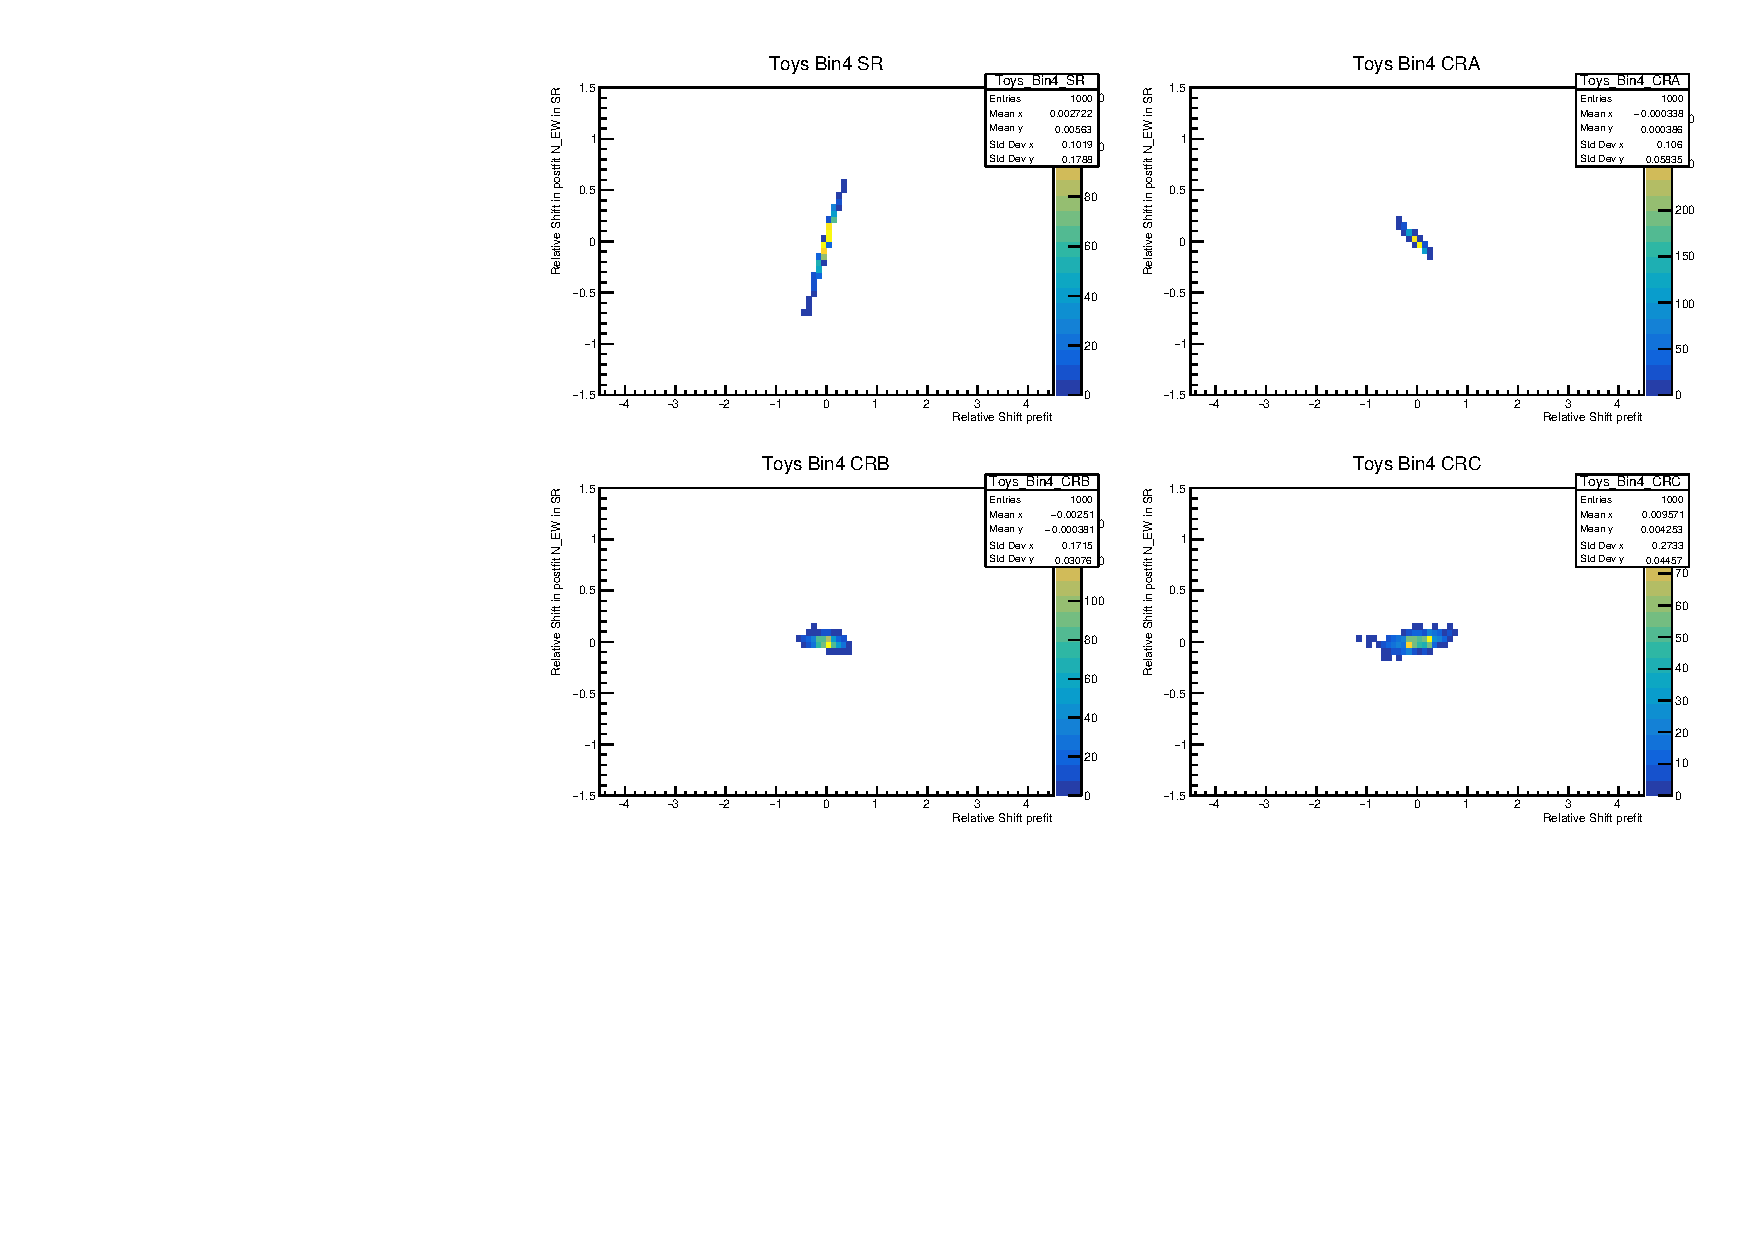
\includegraphics[width=\textwidth]{plots/diffx/instab/constfx/instabilities_mjj_QCD_Sh2211_Signal_Sh2211_BSDATASTATS_sherpaasimov_bin4.pdf}
\end{figure}

\subsubsection{\mjj QCD template fluctuations, MG5 QCD in Asimov, Sherpa-2.2.11 QCD template}
\begin{figure}[H]
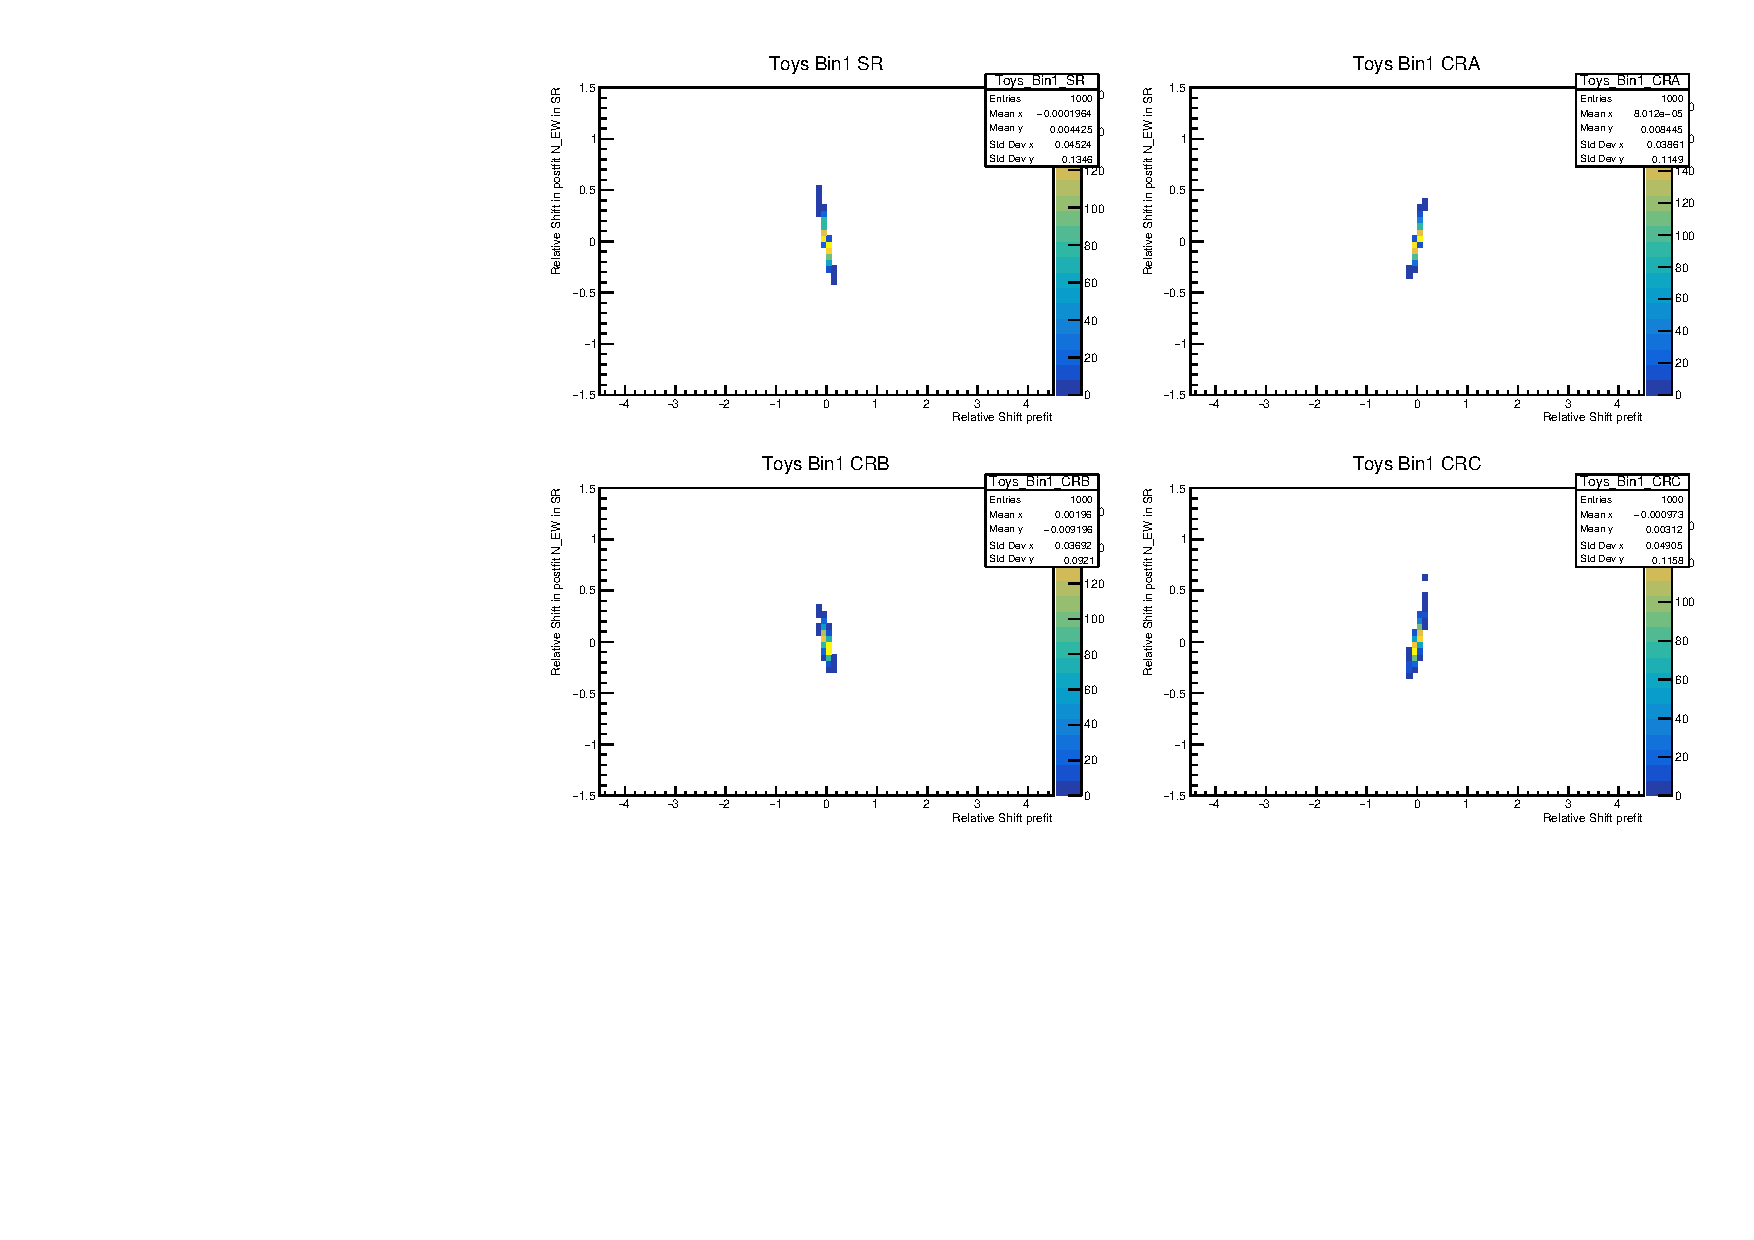
\includegraphics[width=\textwidth]{plots/diffx/instab/constfx/instabilities_mjj_QCD_Sh2211_Signal_Sh2211_BSMCQCDSTATS_madgraphasimov_bin1.pdf}
\end{figure}
\begin{figure}[H]
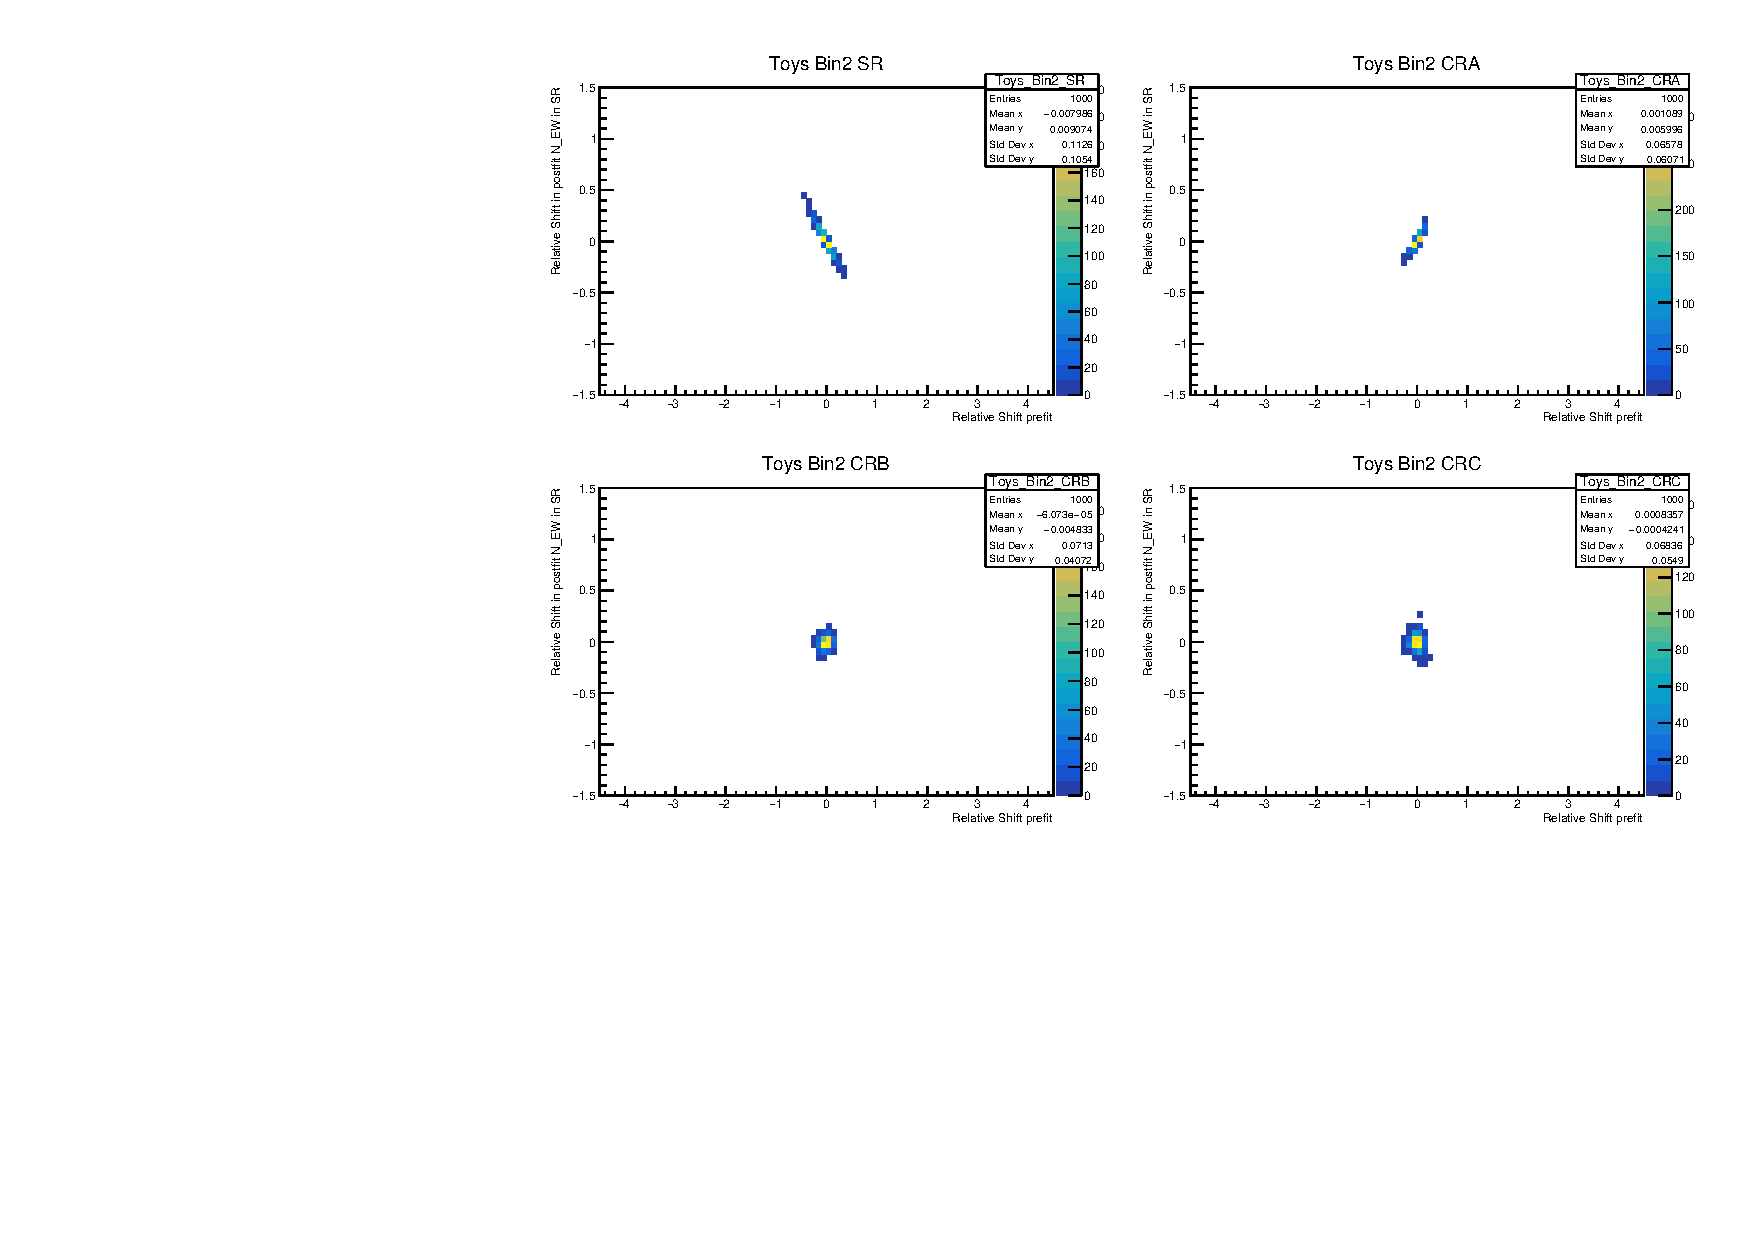
\includegraphics[width=\textwidth]{plots/diffx/instab/constfx/instabilities_mjj_QCD_Sh2211_Signal_Sh2211_BSMCQCDSTATS_madgraphasimov_bin2.pdf}
\end{figure}
\begin{figure}[H]
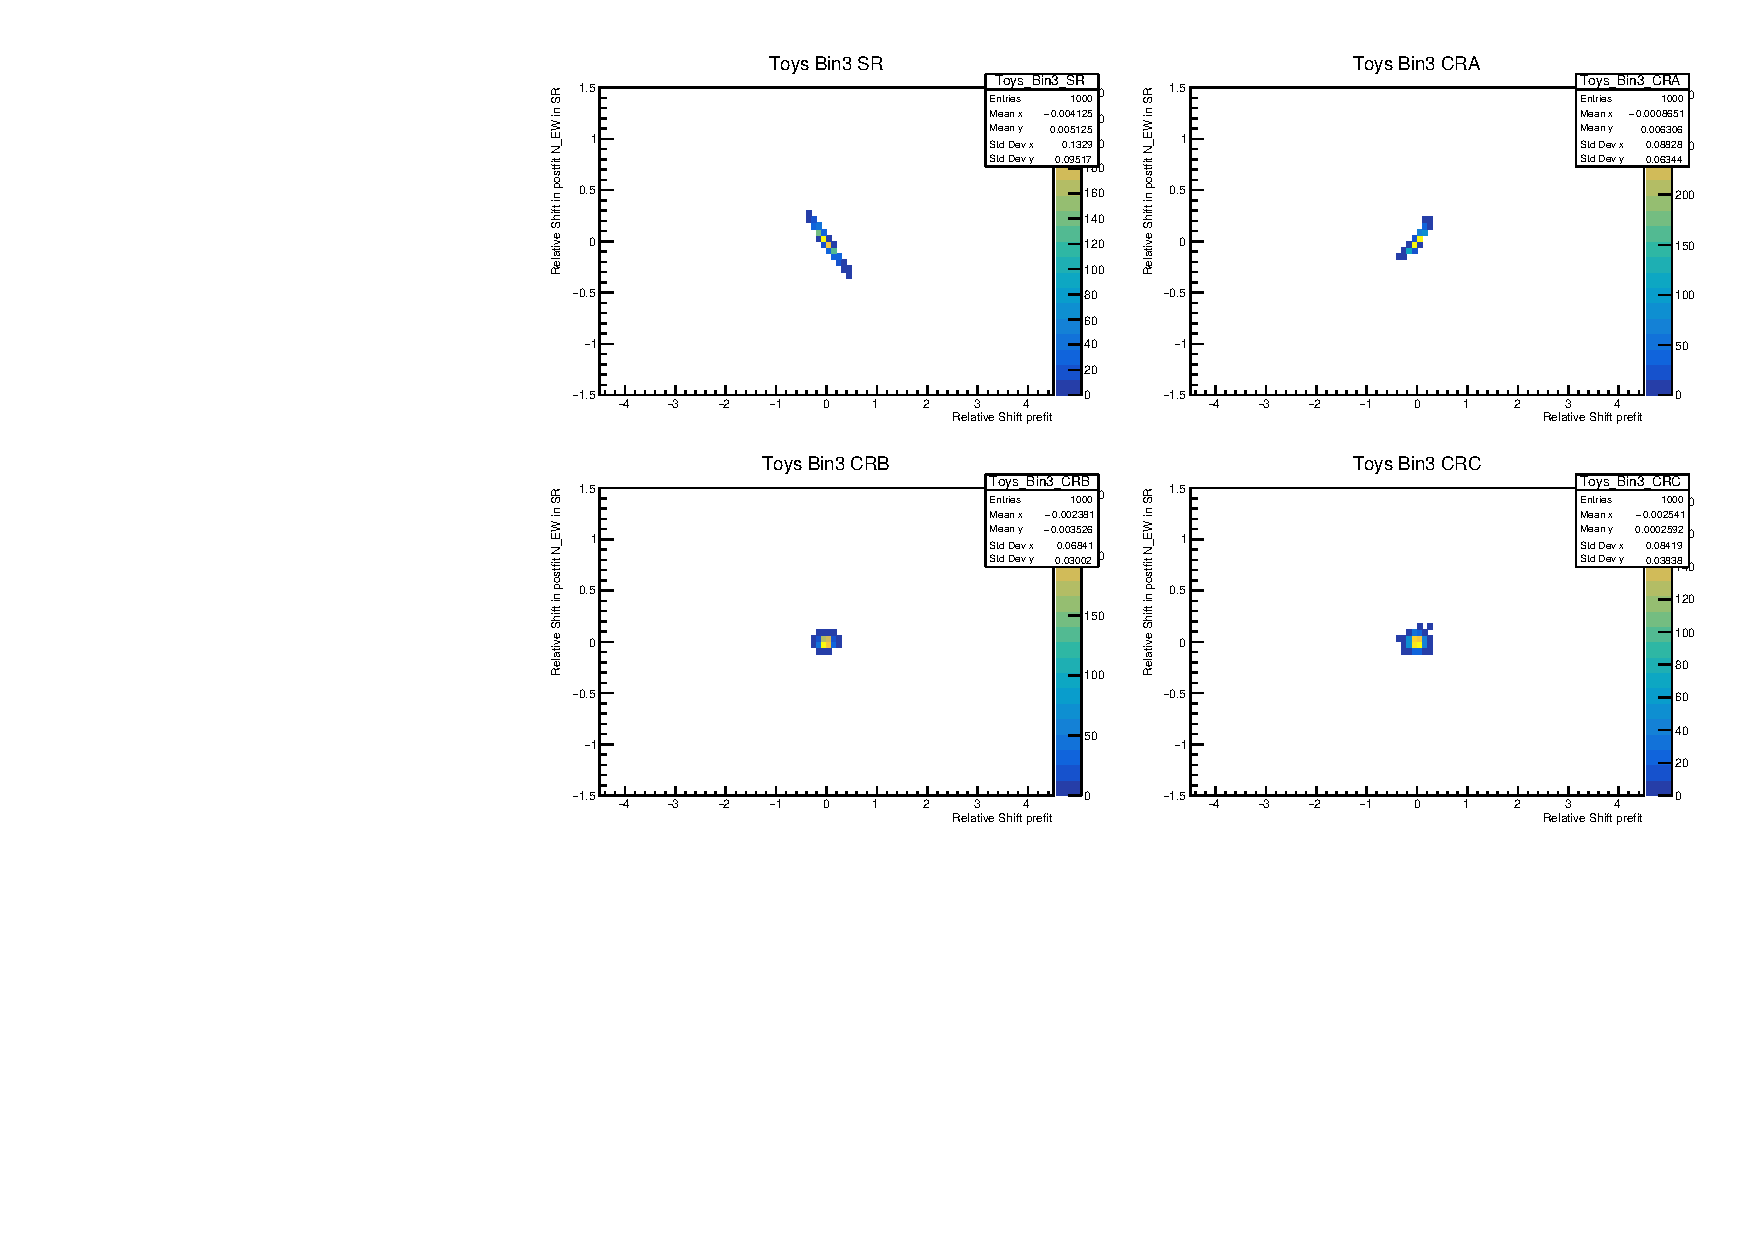
\includegraphics[width=\textwidth]{plots/diffx/instab/constfx/instabilities_mjj_QCD_Sh2211_Signal_Sh2211_BSMCQCDSTATS_madgraphasimov_bin3.pdf}
\end{figure}
\begin{figure}[H]
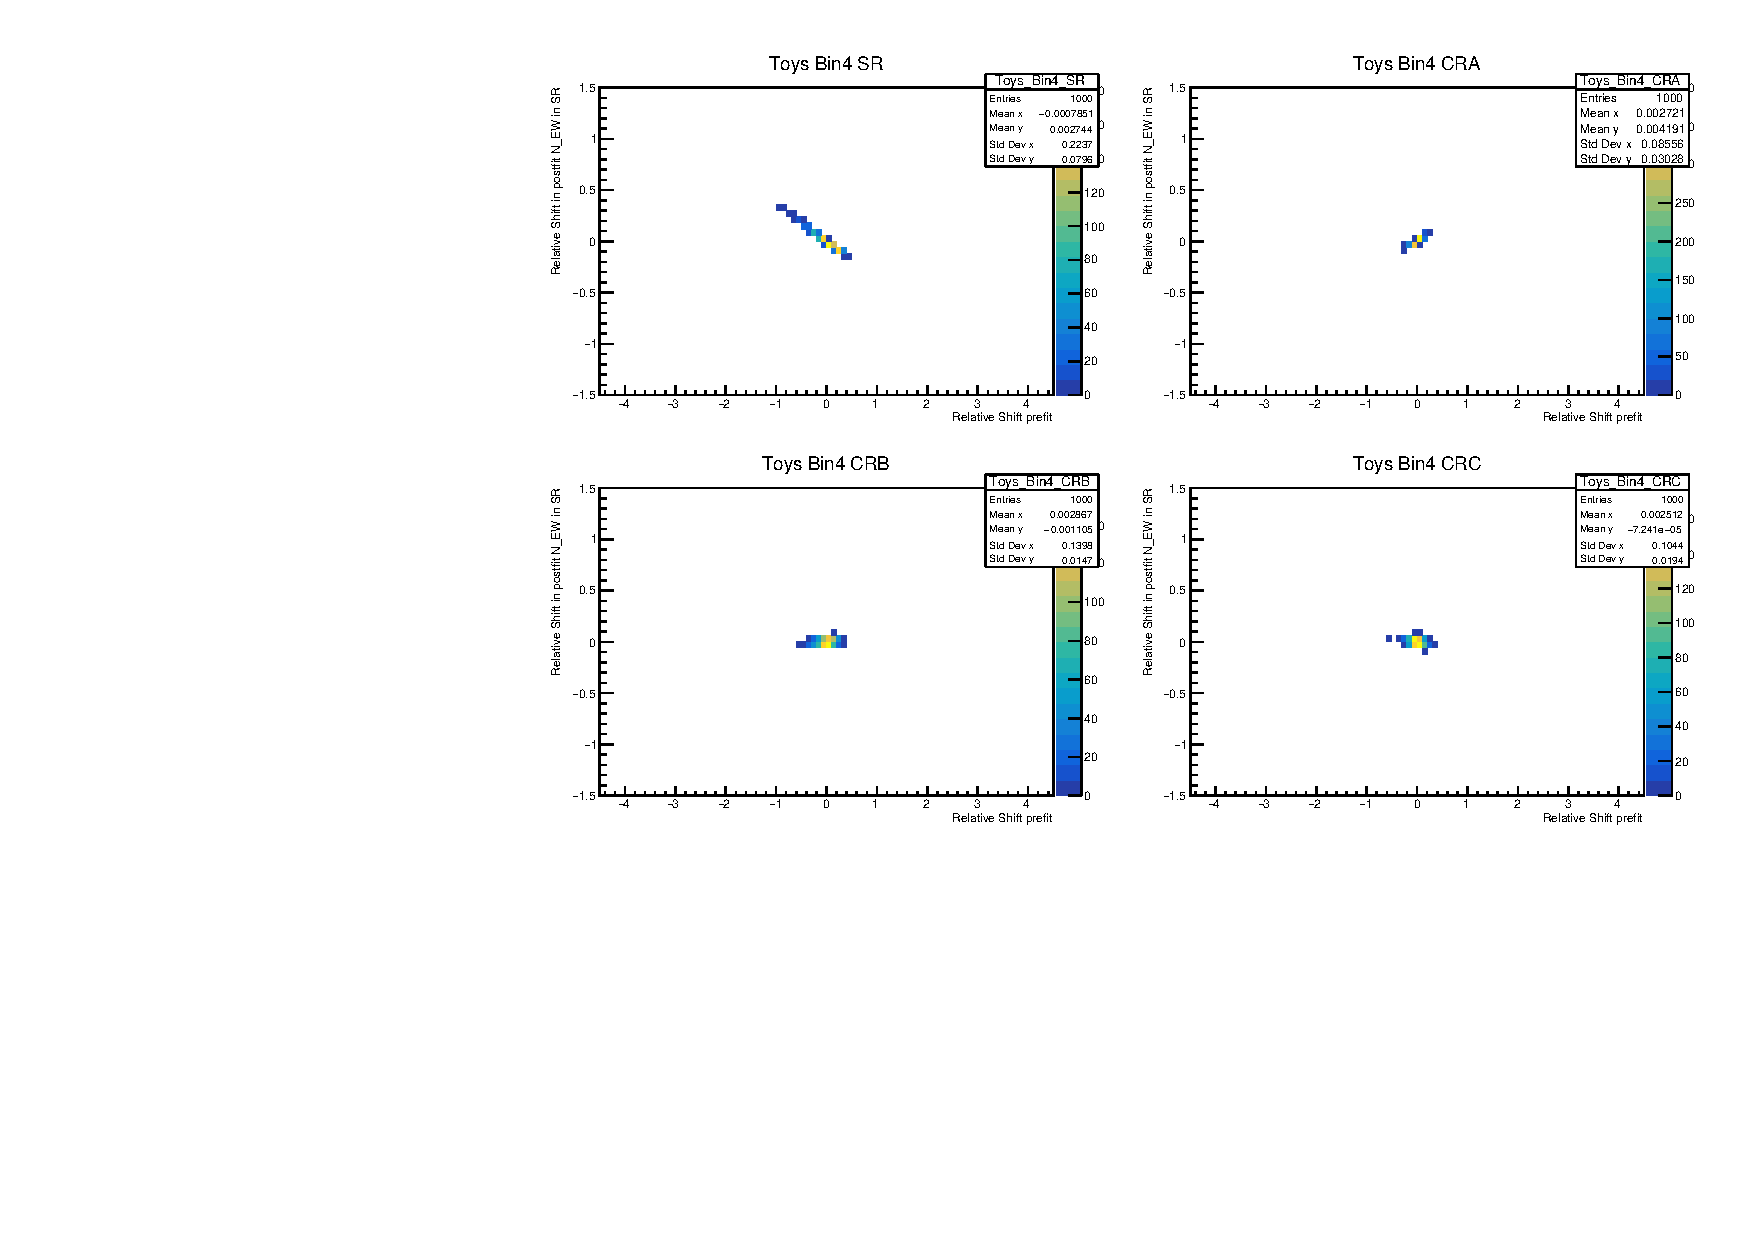
\includegraphics[width=\textwidth]{plots/diffx/instab/constfx/instabilities_mjj_QCD_Sh2211_Signal_Sh2211_BSMCQCDSTATS_madgraphasimov_bin4.pdf}
\end{figure}

\subsubsection{\mjj QCD template fluctuations, Sherpa-2.2.11 QCD in Asimov, Sherpa-2.2.11 QCD template}
\begin{figure}[H]
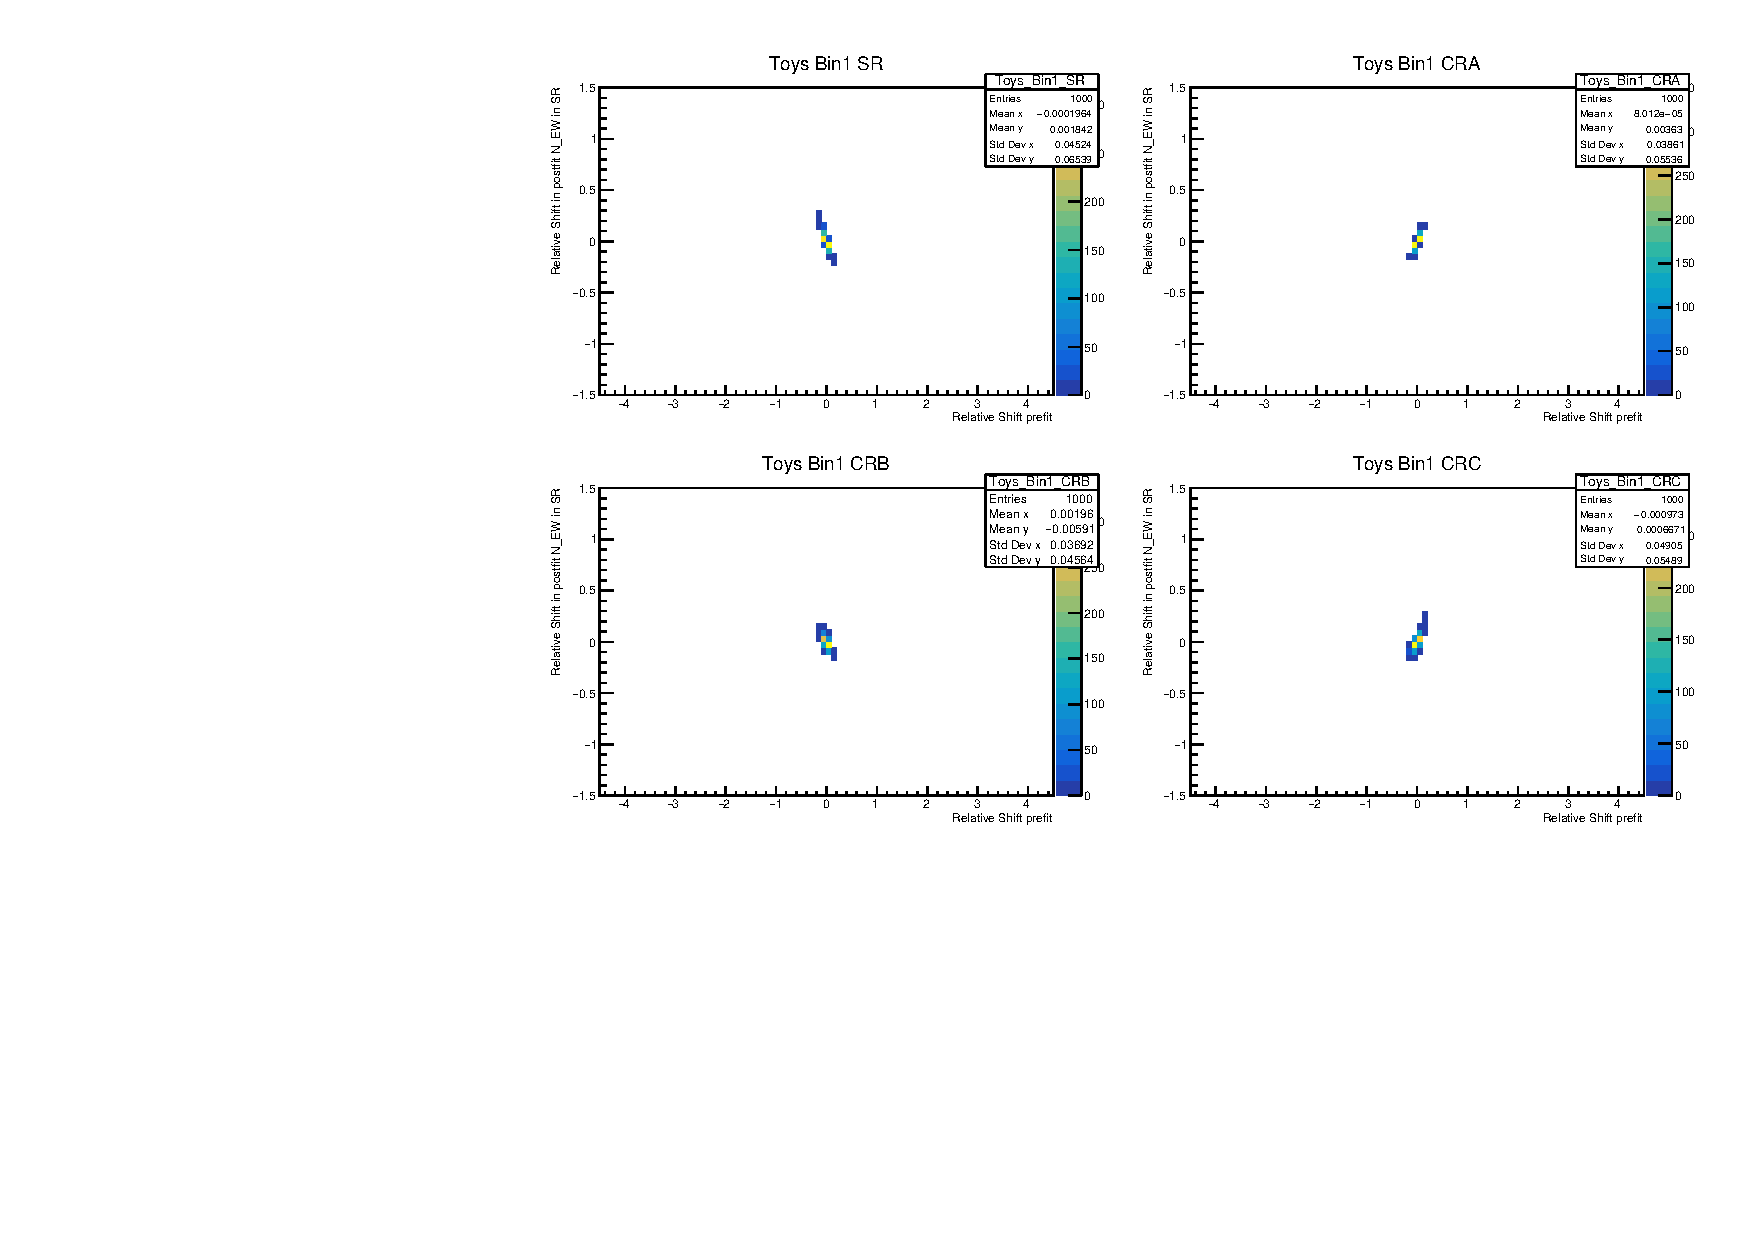
\includegraphics[width=\textwidth]{plots/diffx/instab/constfx/instabilities_mjj_QCD_Sh2211_Signal_Sh2211_BSMCQCDSTATS_sherpaasimov_bin1.pdf}
\end{figure}
\begin{figure}[H]
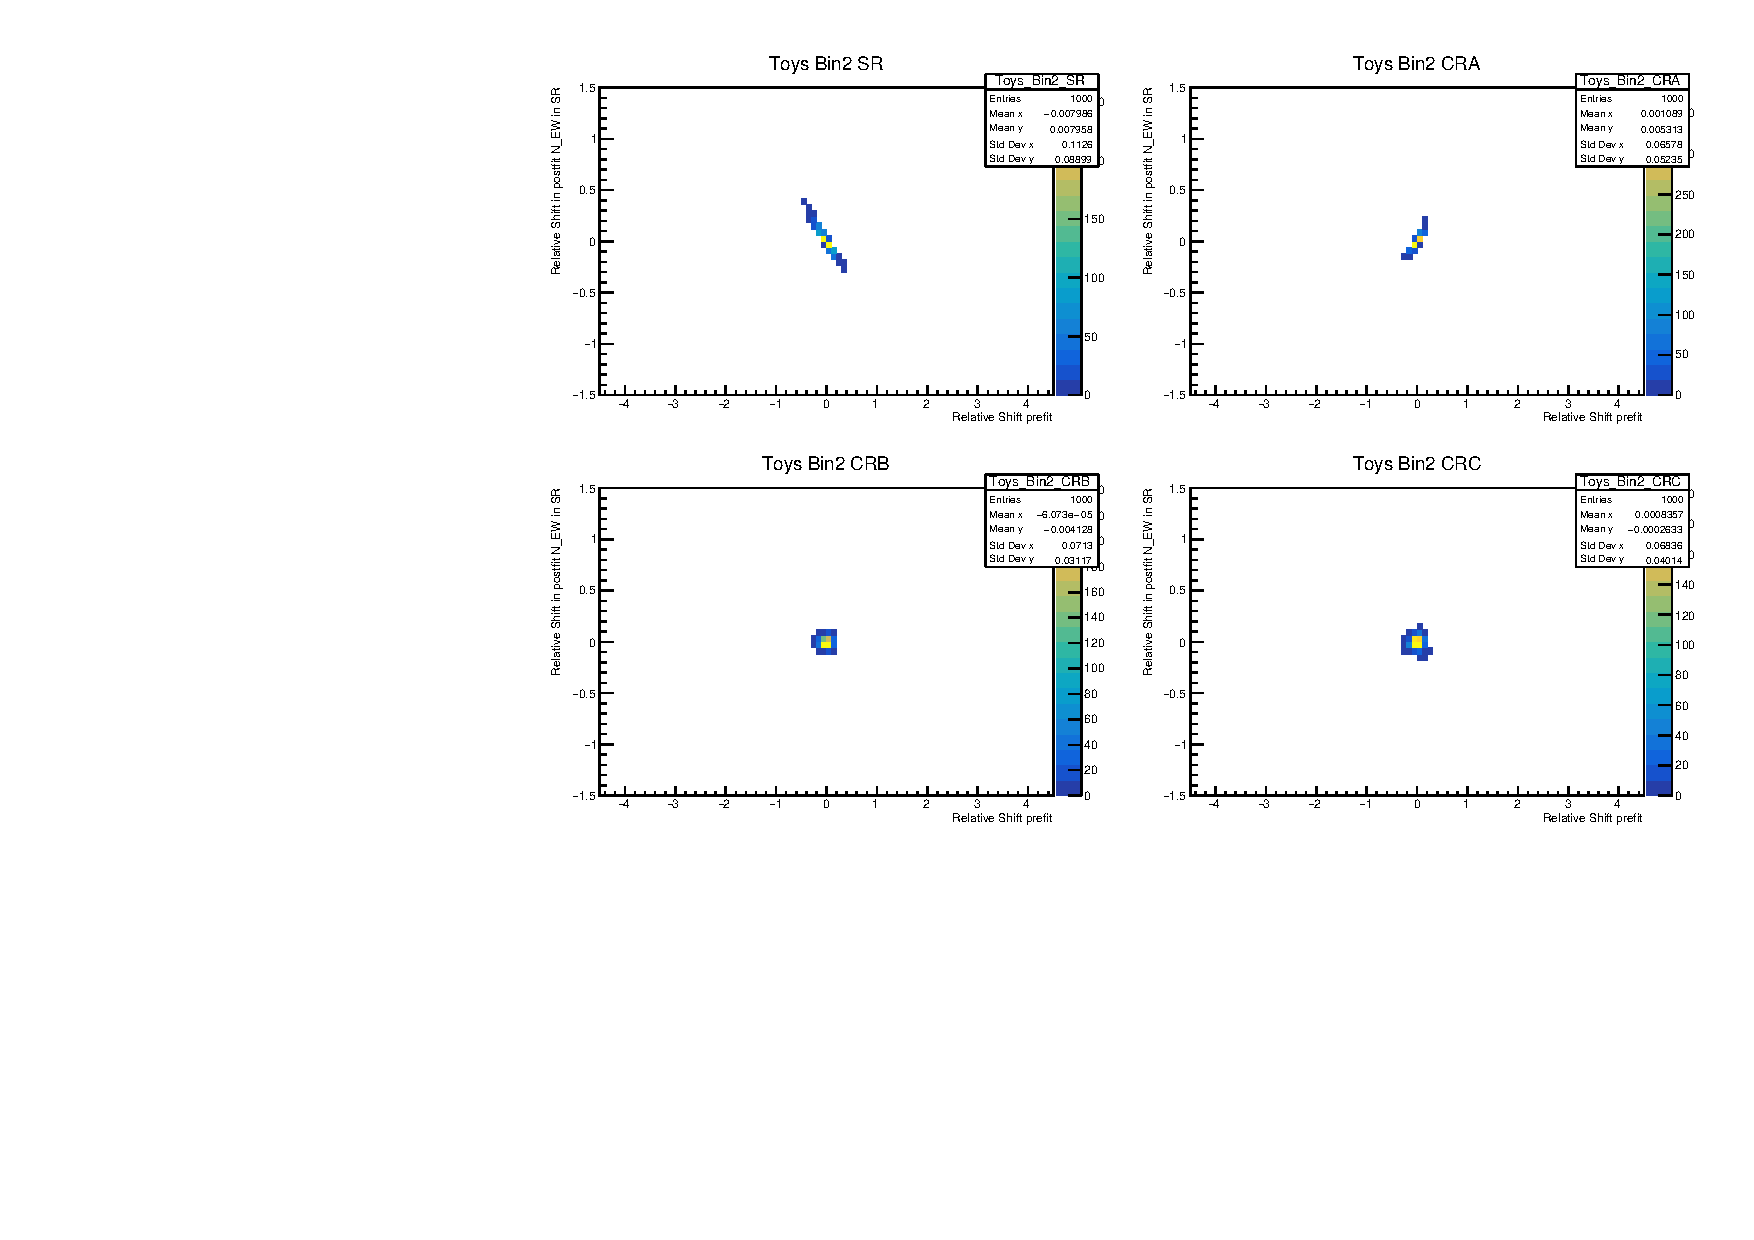
\includegraphics[width=\textwidth]{plots/diffx/instab/constfx/instabilities_mjj_QCD_Sh2211_Signal_Sh2211_BSMCQCDSTATS_sherpaasimov_bin2.pdf}
\end{figure}
\begin{figure}[H]
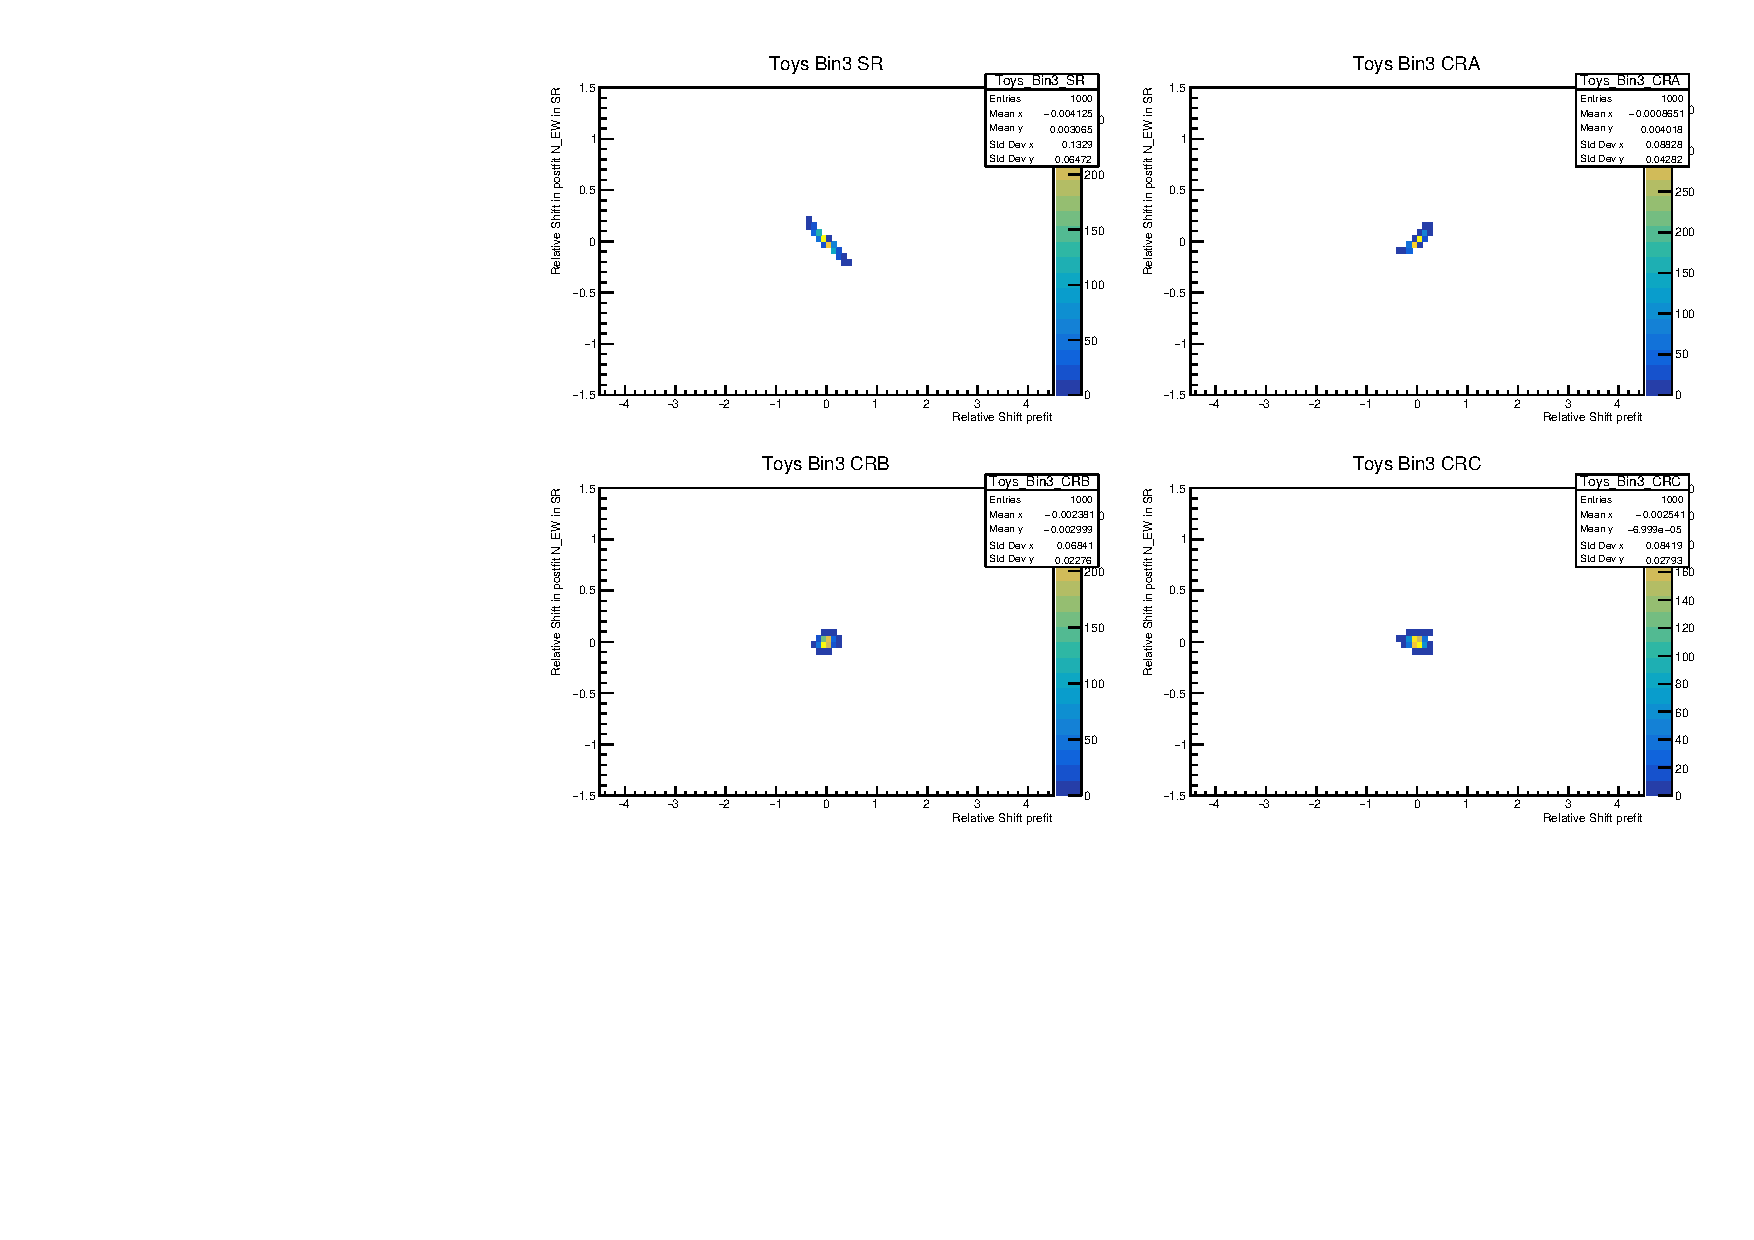
\includegraphics[width=\textwidth]{plots/diffx/instab/constfx/instabilities_mjj_QCD_Sh2211_Signal_Sh2211_BSMCQCDSTATS_sherpaasimov_bin3.pdf}
\end{figure}
\begin{figure}[H]
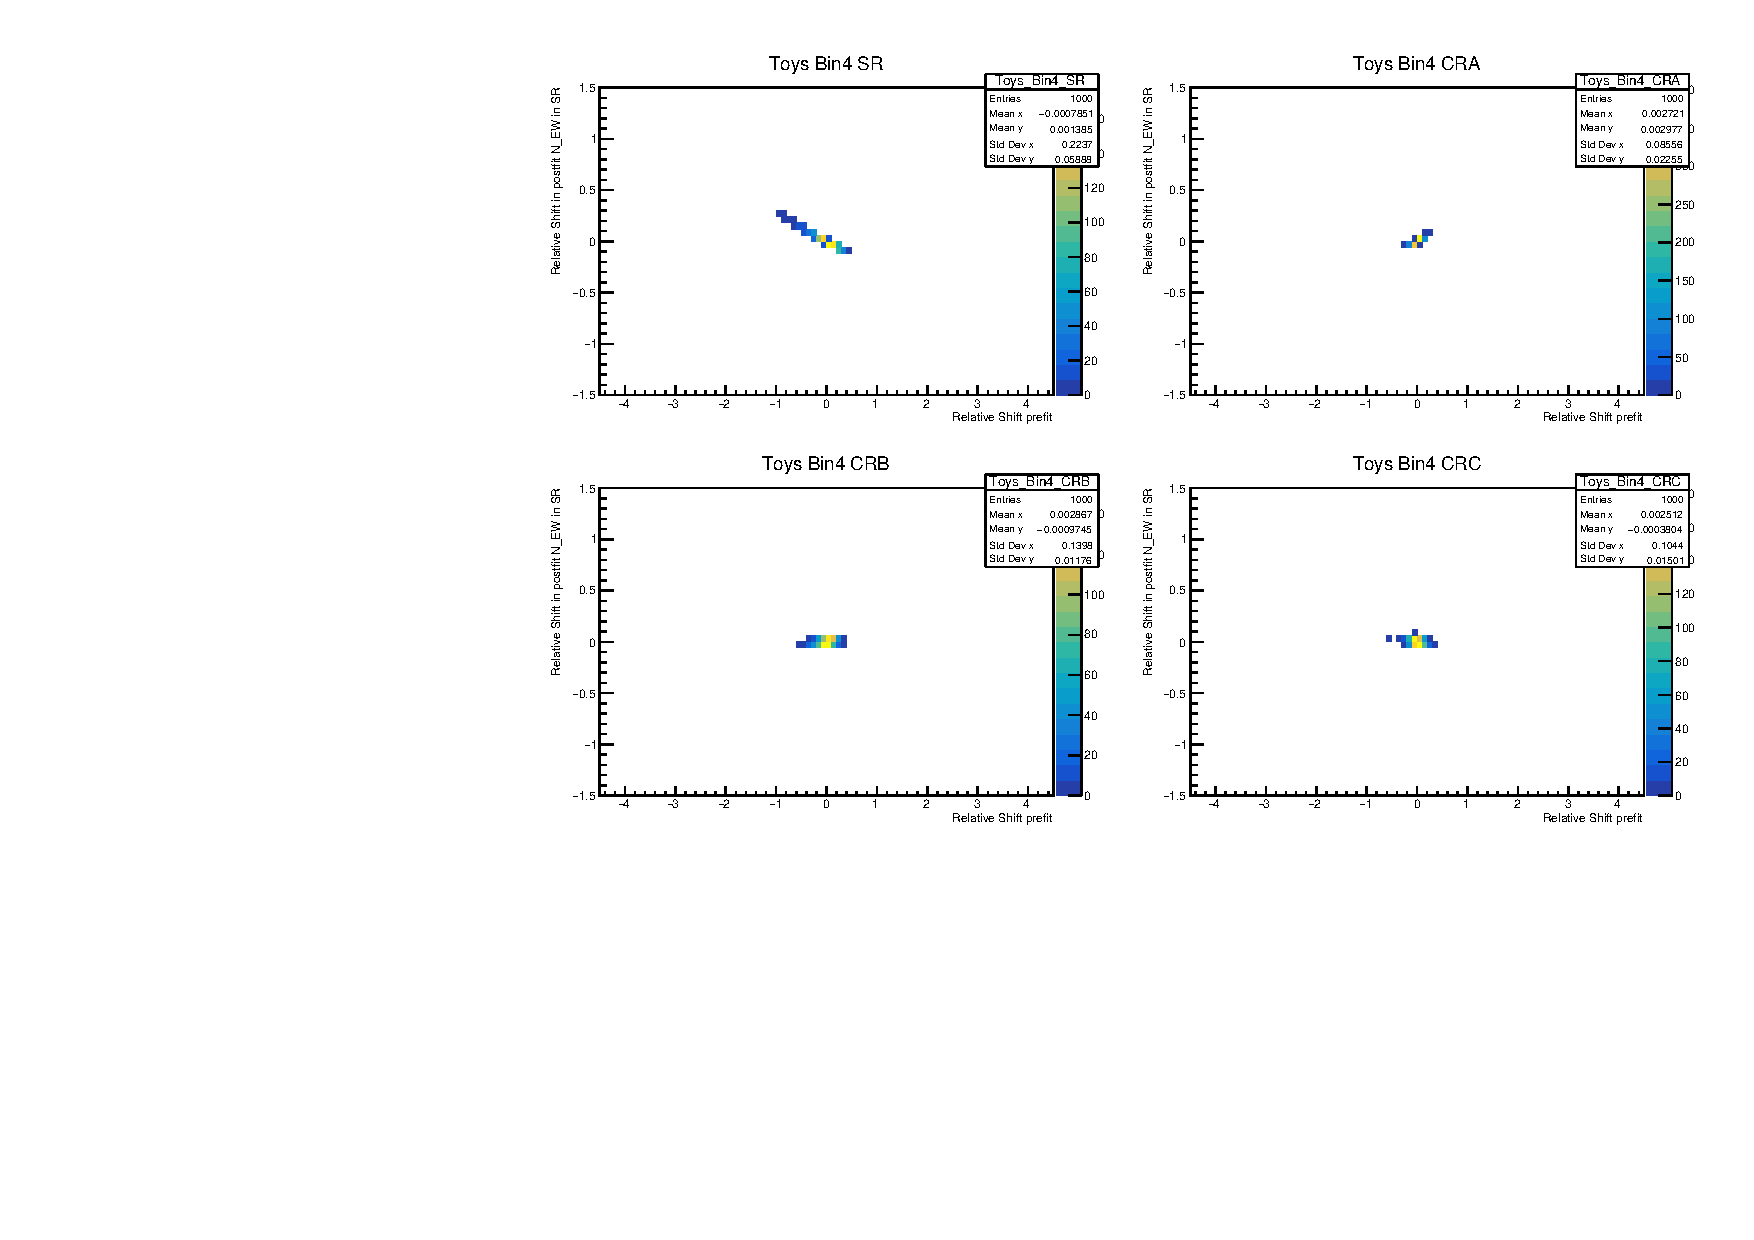
\includegraphics[width=\textwidth]{plots/diffx/instab/constfx/instabilities_mjj_QCD_Sh2211_Signal_Sh2211_BSMCQCDSTATS_sherpaasimov_bin4.pdf}
\end{figure}

\subsection{$\fx=mx_i+c$\label{sec:appendix:stability:fxlinear}}
\subsubsection{\mjj Asimov fluctuations, MG5 QCD in Asimov, MG5 QCD template}
\begin{figure}[H]
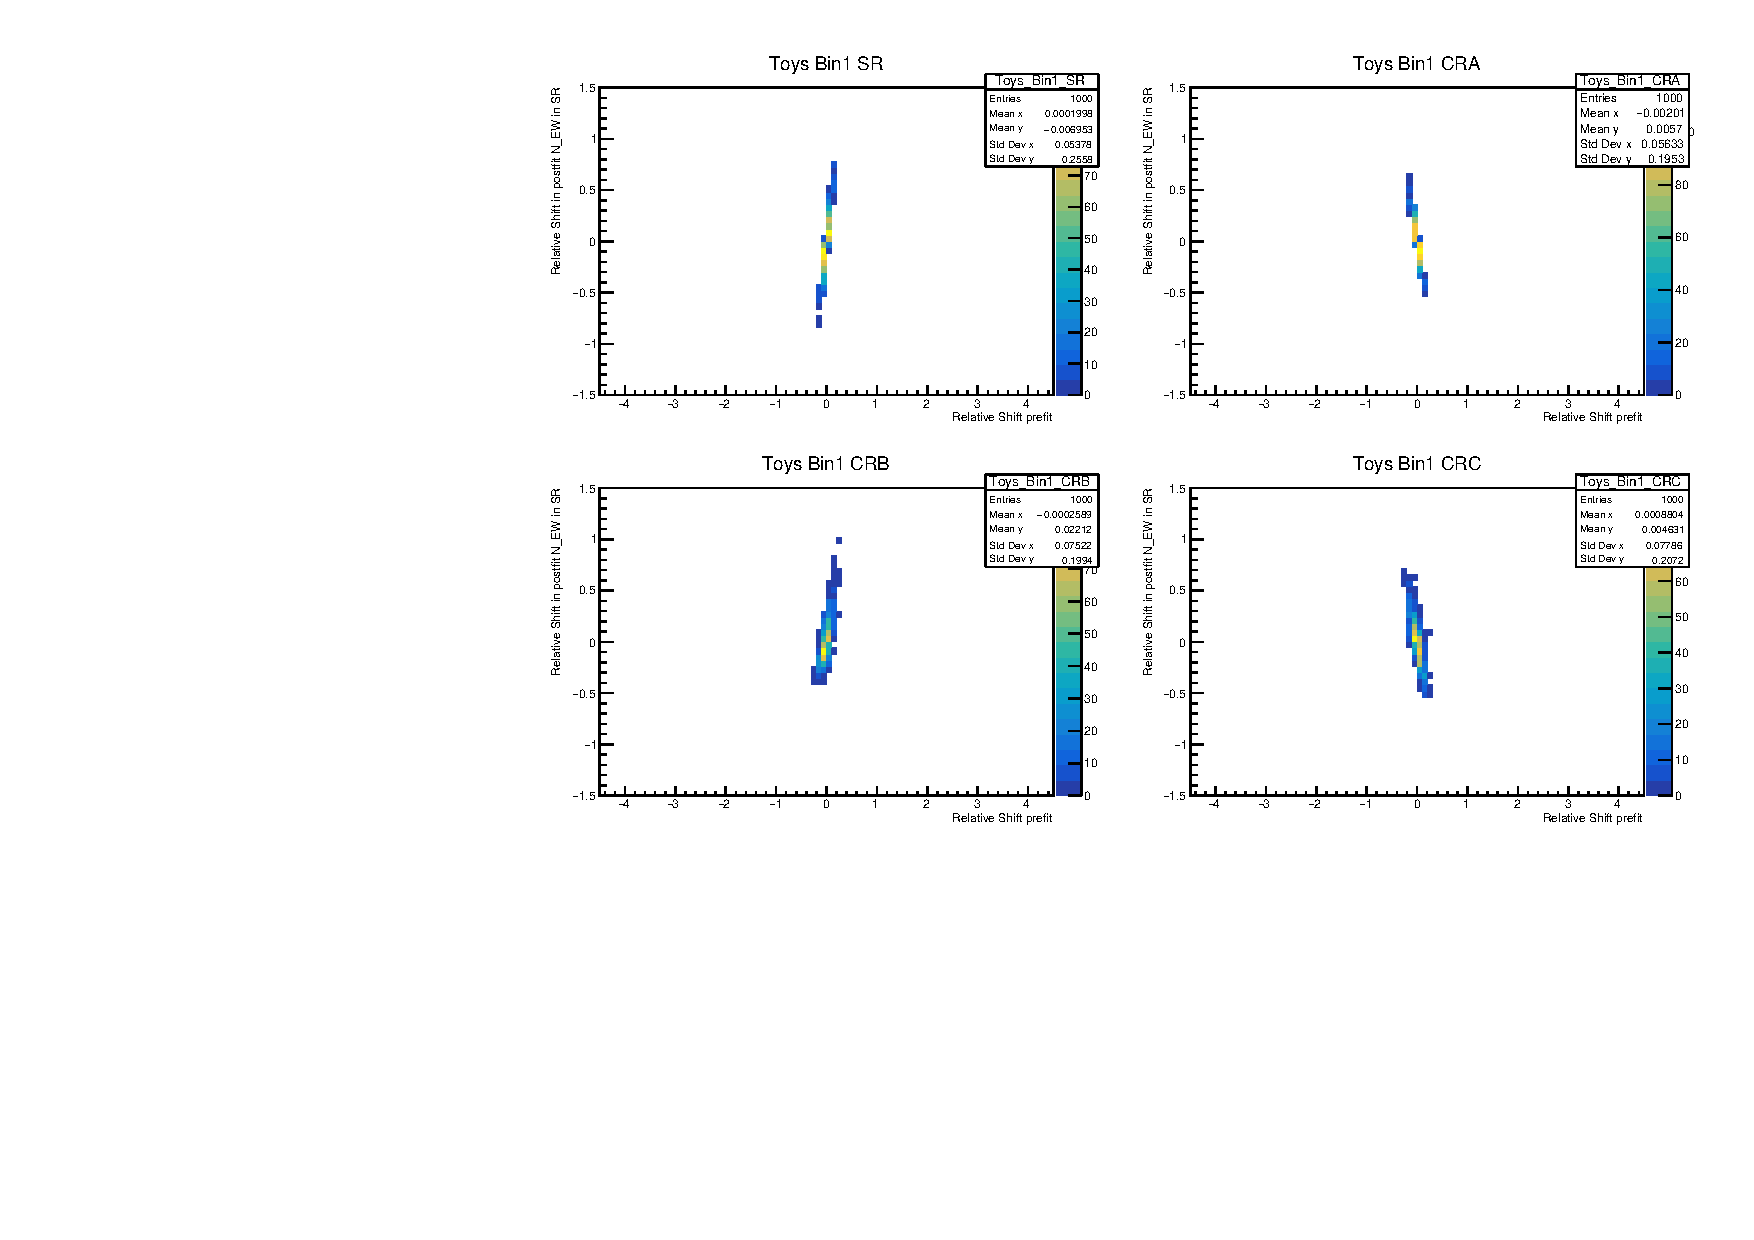
\includegraphics[width=\textwidth]{plots/diffx/instab/linearfx/instabilities_mjj_QCD_Mgraph_Signal_Sh2211_BSDATASTATS_linearfx_newbinning_madgraphasimov_bin1.pdf}
\end{figure}
\begin{figure}[H]
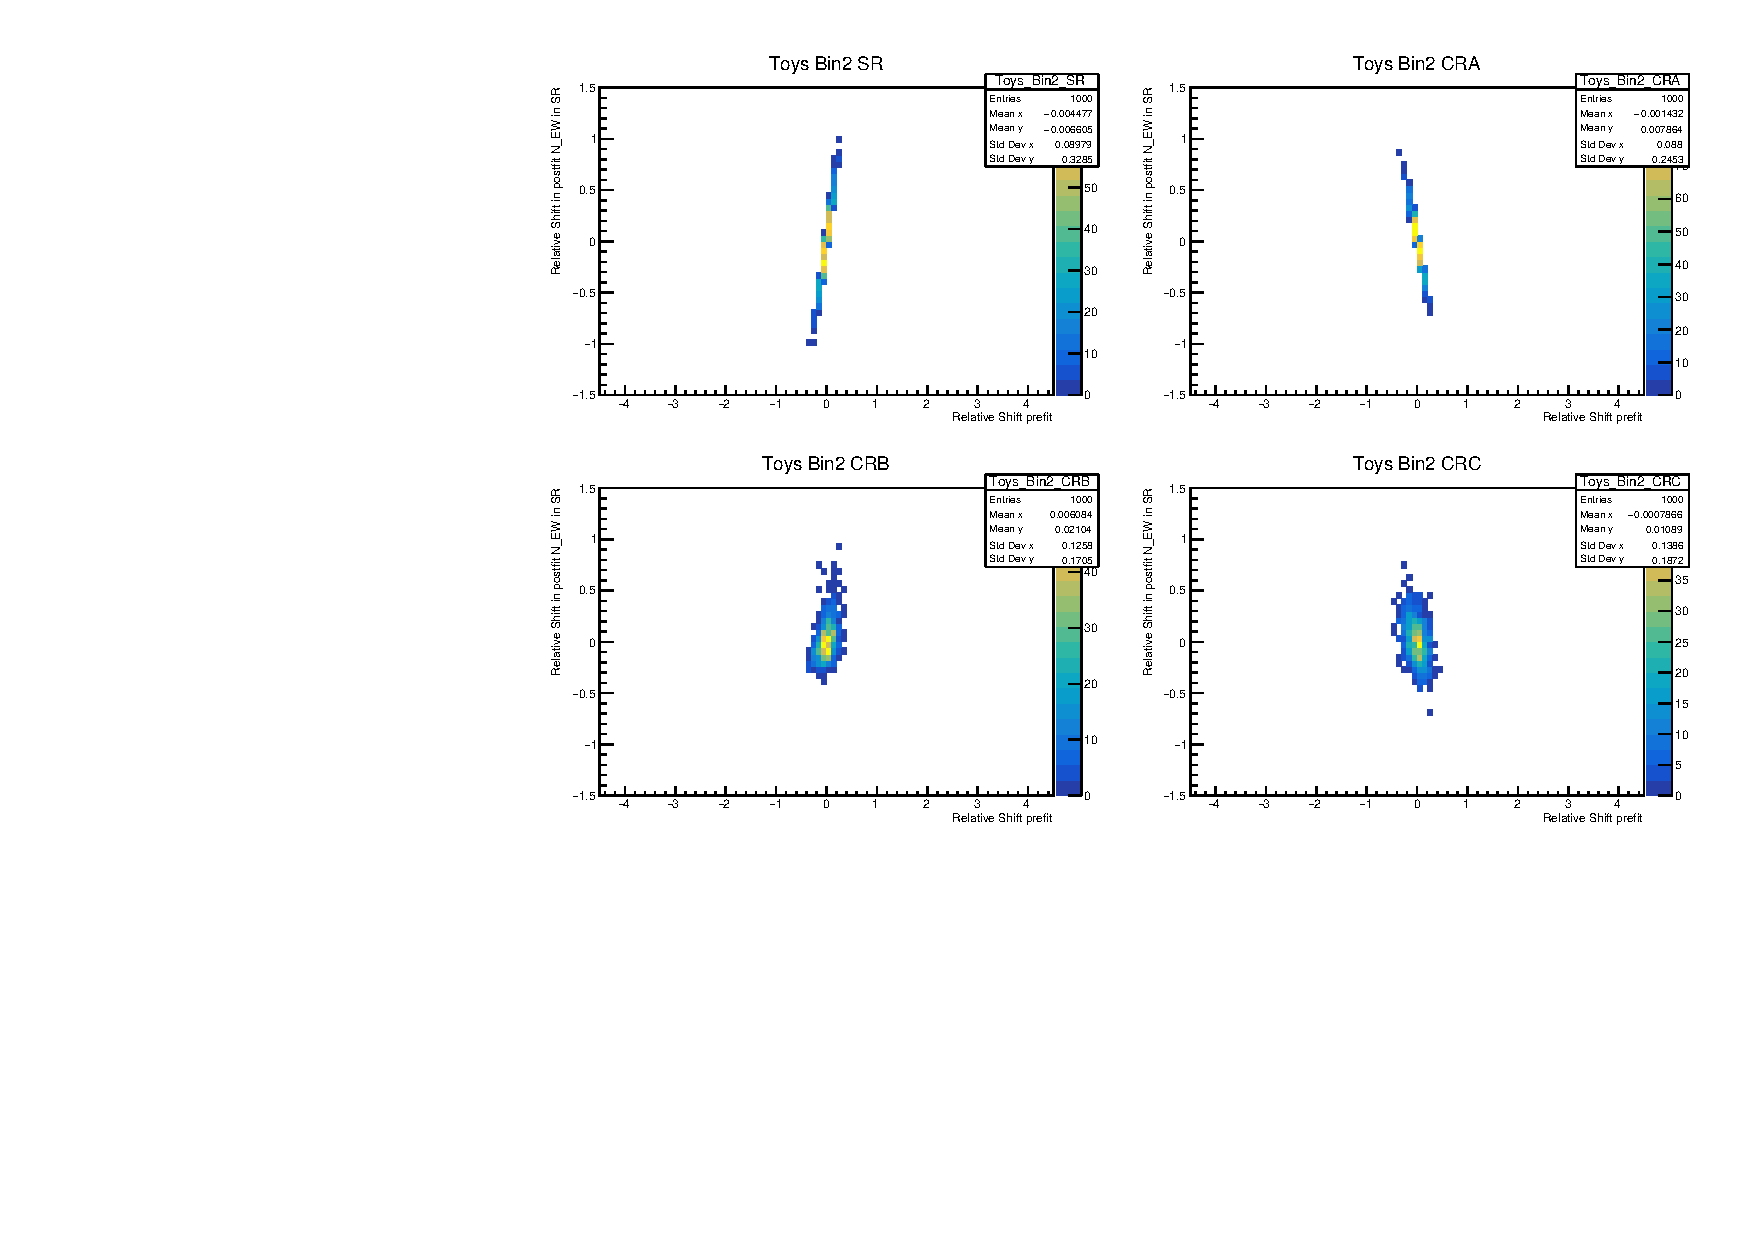
\includegraphics[width=\textwidth]{plots/diffx/instab/linearfx/instabilities_mjj_QCD_Mgraph_Signal_Sh2211_BSDATASTATS_linearfx_newbinning_madgraphasimov_bin2.pdf}
\end{figure}
\begin{figure}[H]
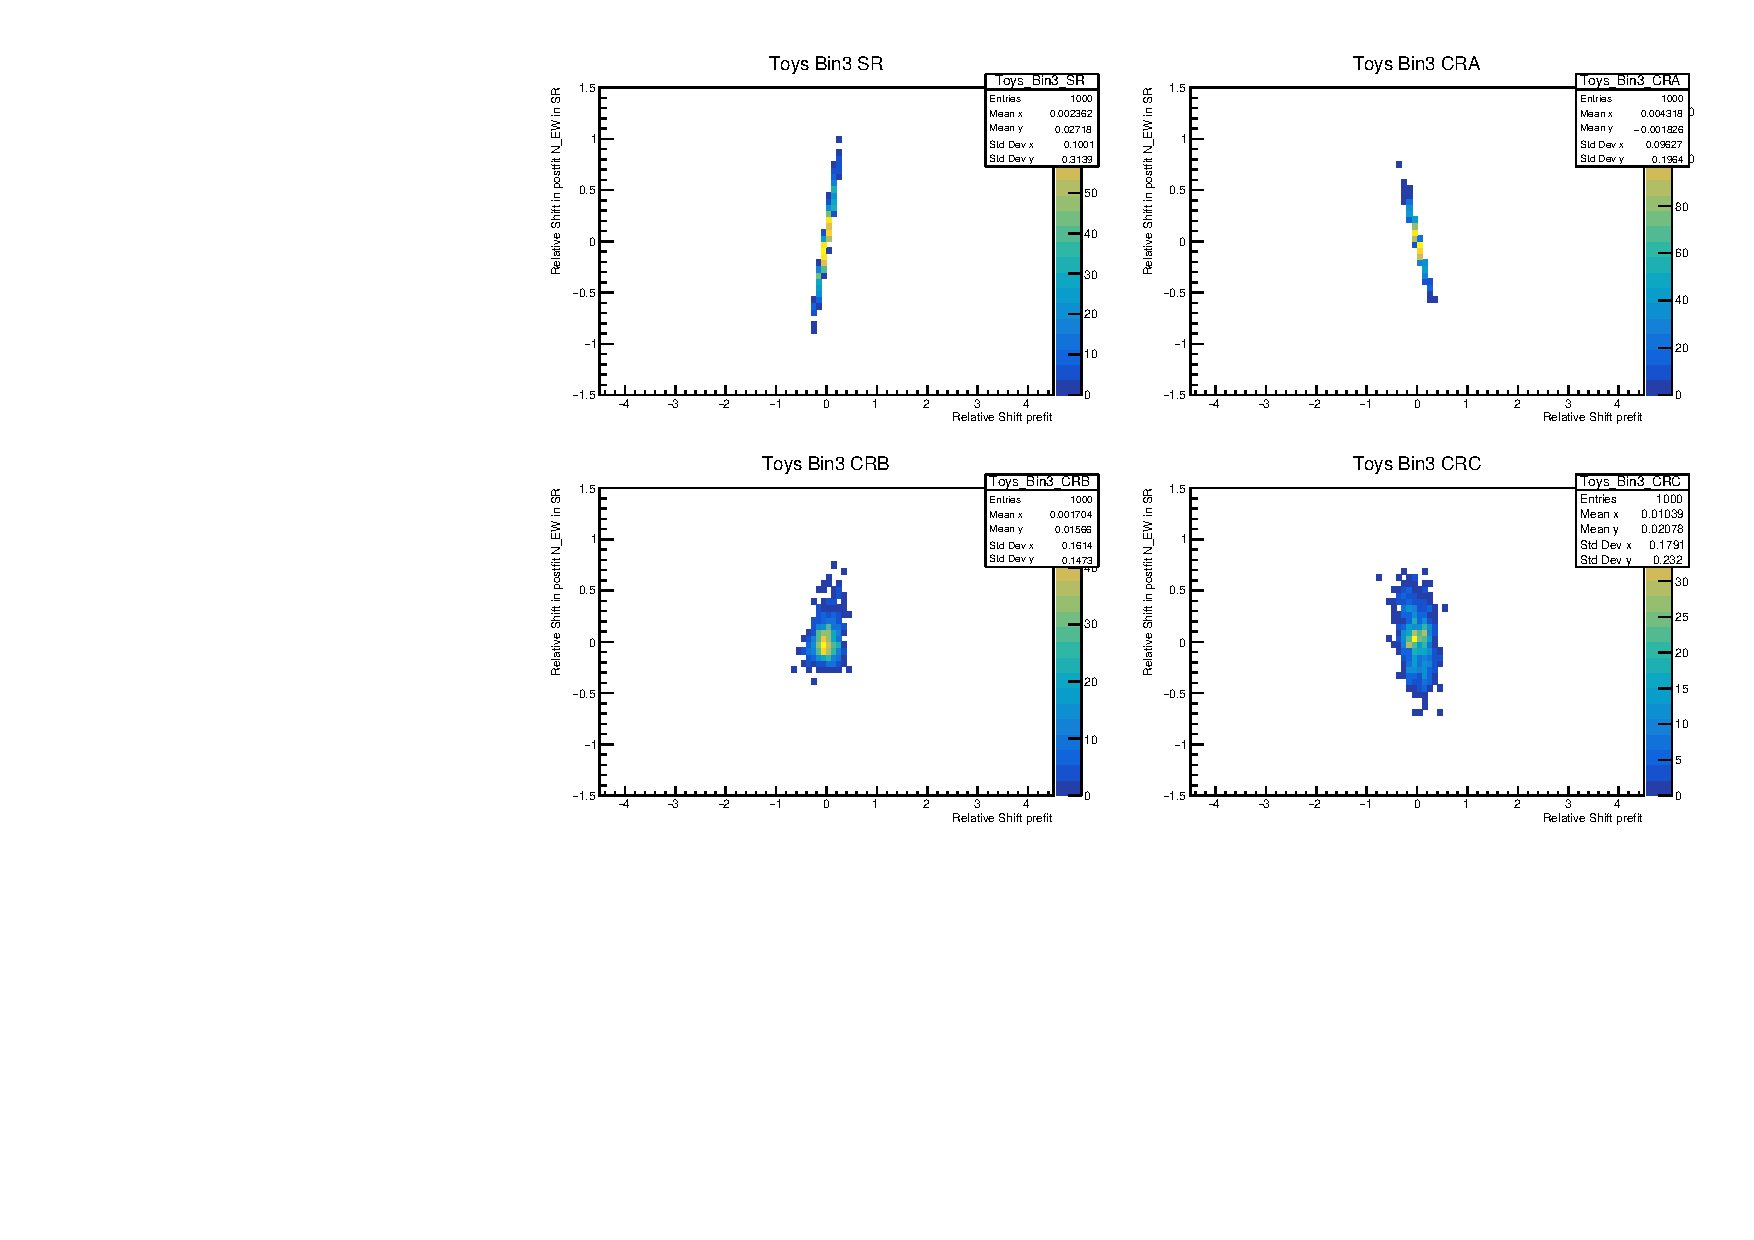
\includegraphics[width=\textwidth]{plots/diffx/instab/linearfx/instabilities_mjj_QCD_Mgraph_Signal_Sh2211_BSDATASTATS_linearfx_newbinning_madgraphasimov_bin3.pdf}
\end{figure}
\begin{figure}[H]
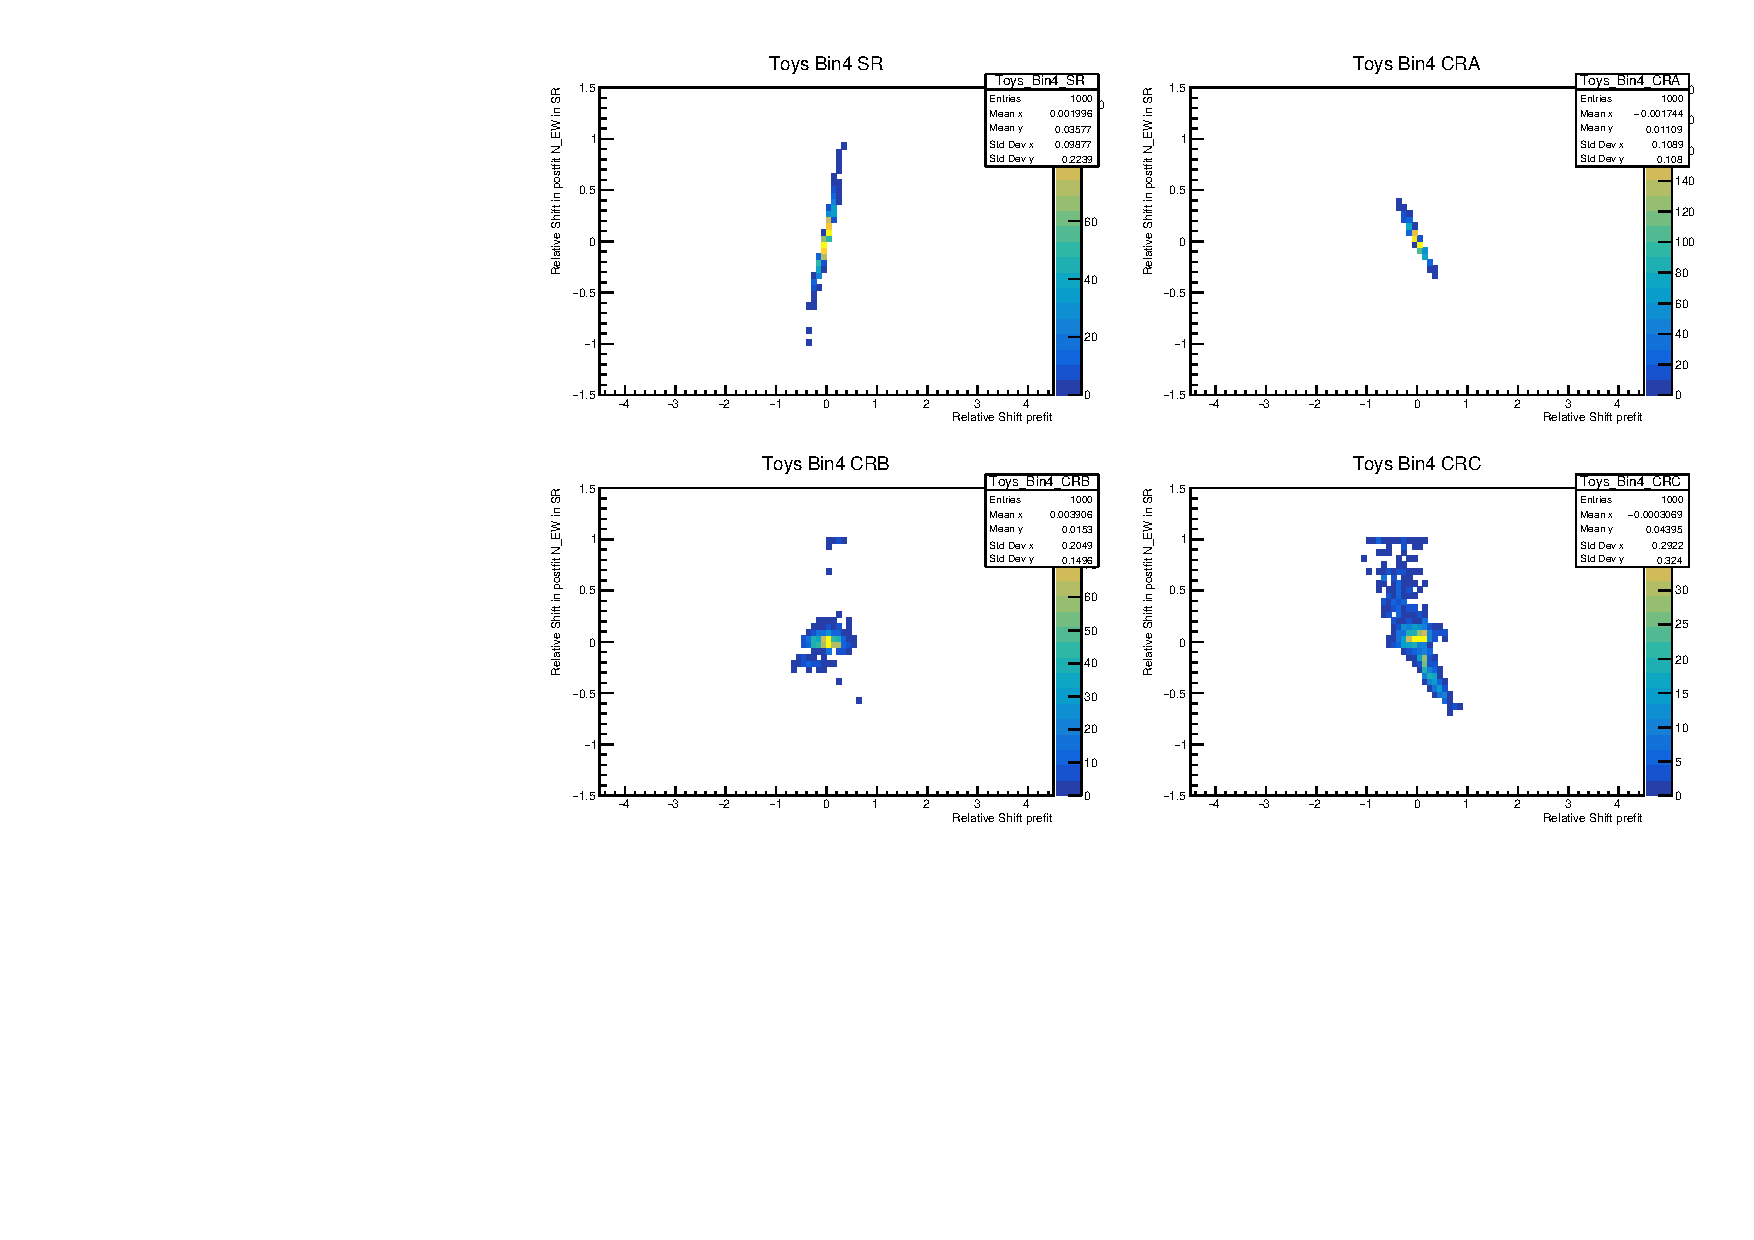
\includegraphics[width=\textwidth]{plots/diffx/instab/linearfx/instabilities_mjj_QCD_Mgraph_Signal_Sh2211_BSDATASTATS_linearfx_newbinning_madgraphasimov_bin4.pdf}
\end{figure}

\subsubsection{\mjj Asimov fluctuations, Sherpa-2.2.11 QCD in Asimov, MG5 QCD template}
\begin{figure}[H]
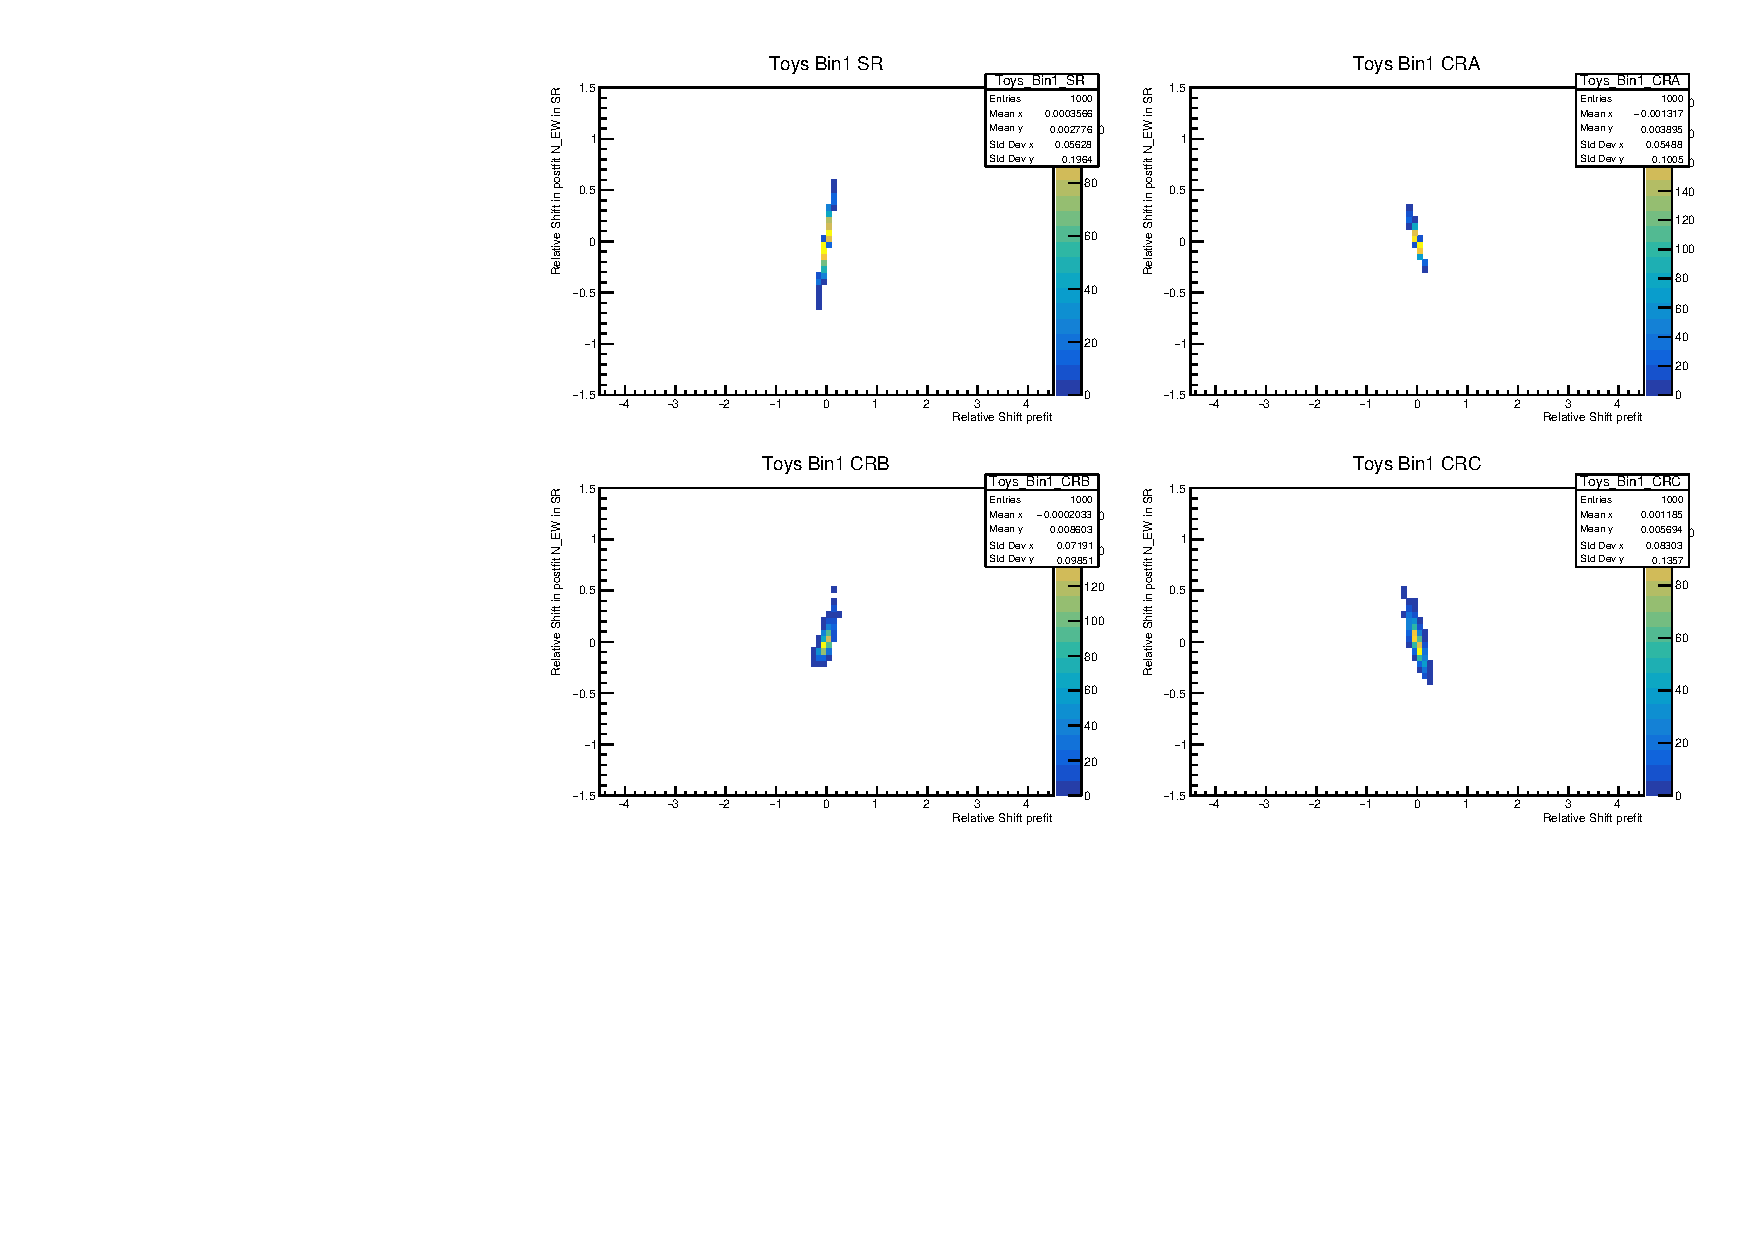
\includegraphics[width=\textwidth]{plots/diffx/instab/linearfx/instabilities_mjj_QCD_Mgraph_Signal_Sh2211_BSDATASTATS_linearfx_newbinning_sherpaasimov_bin1.pdf}
\end{figure}
\begin{figure}[H]
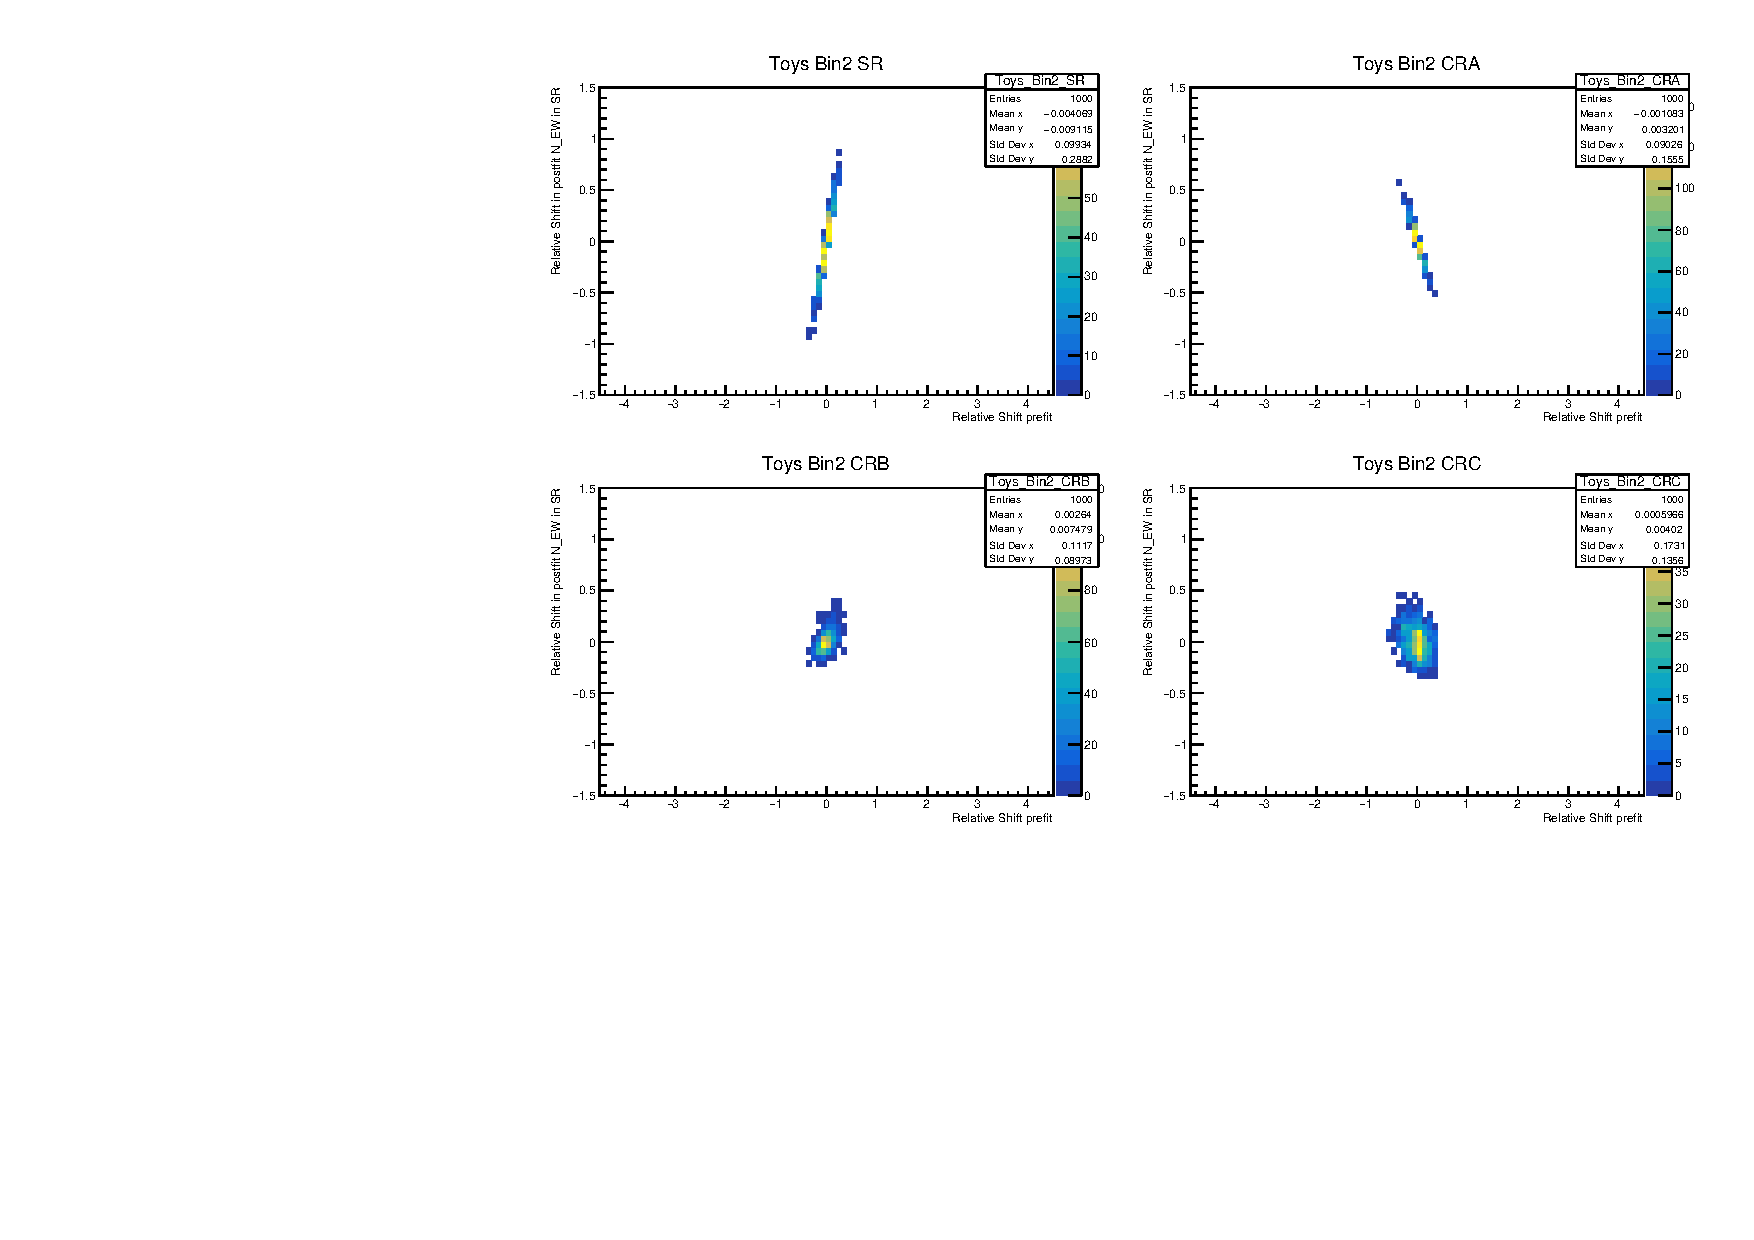
\includegraphics[width=\textwidth]{plots/diffx/instab/linearfx/instabilities_mjj_QCD_Mgraph_Signal_Sh2211_BSDATASTATS_linearfx_newbinning_sherpaasimov_bin2.pdf}
\end{figure}
\begin{figure}[H]
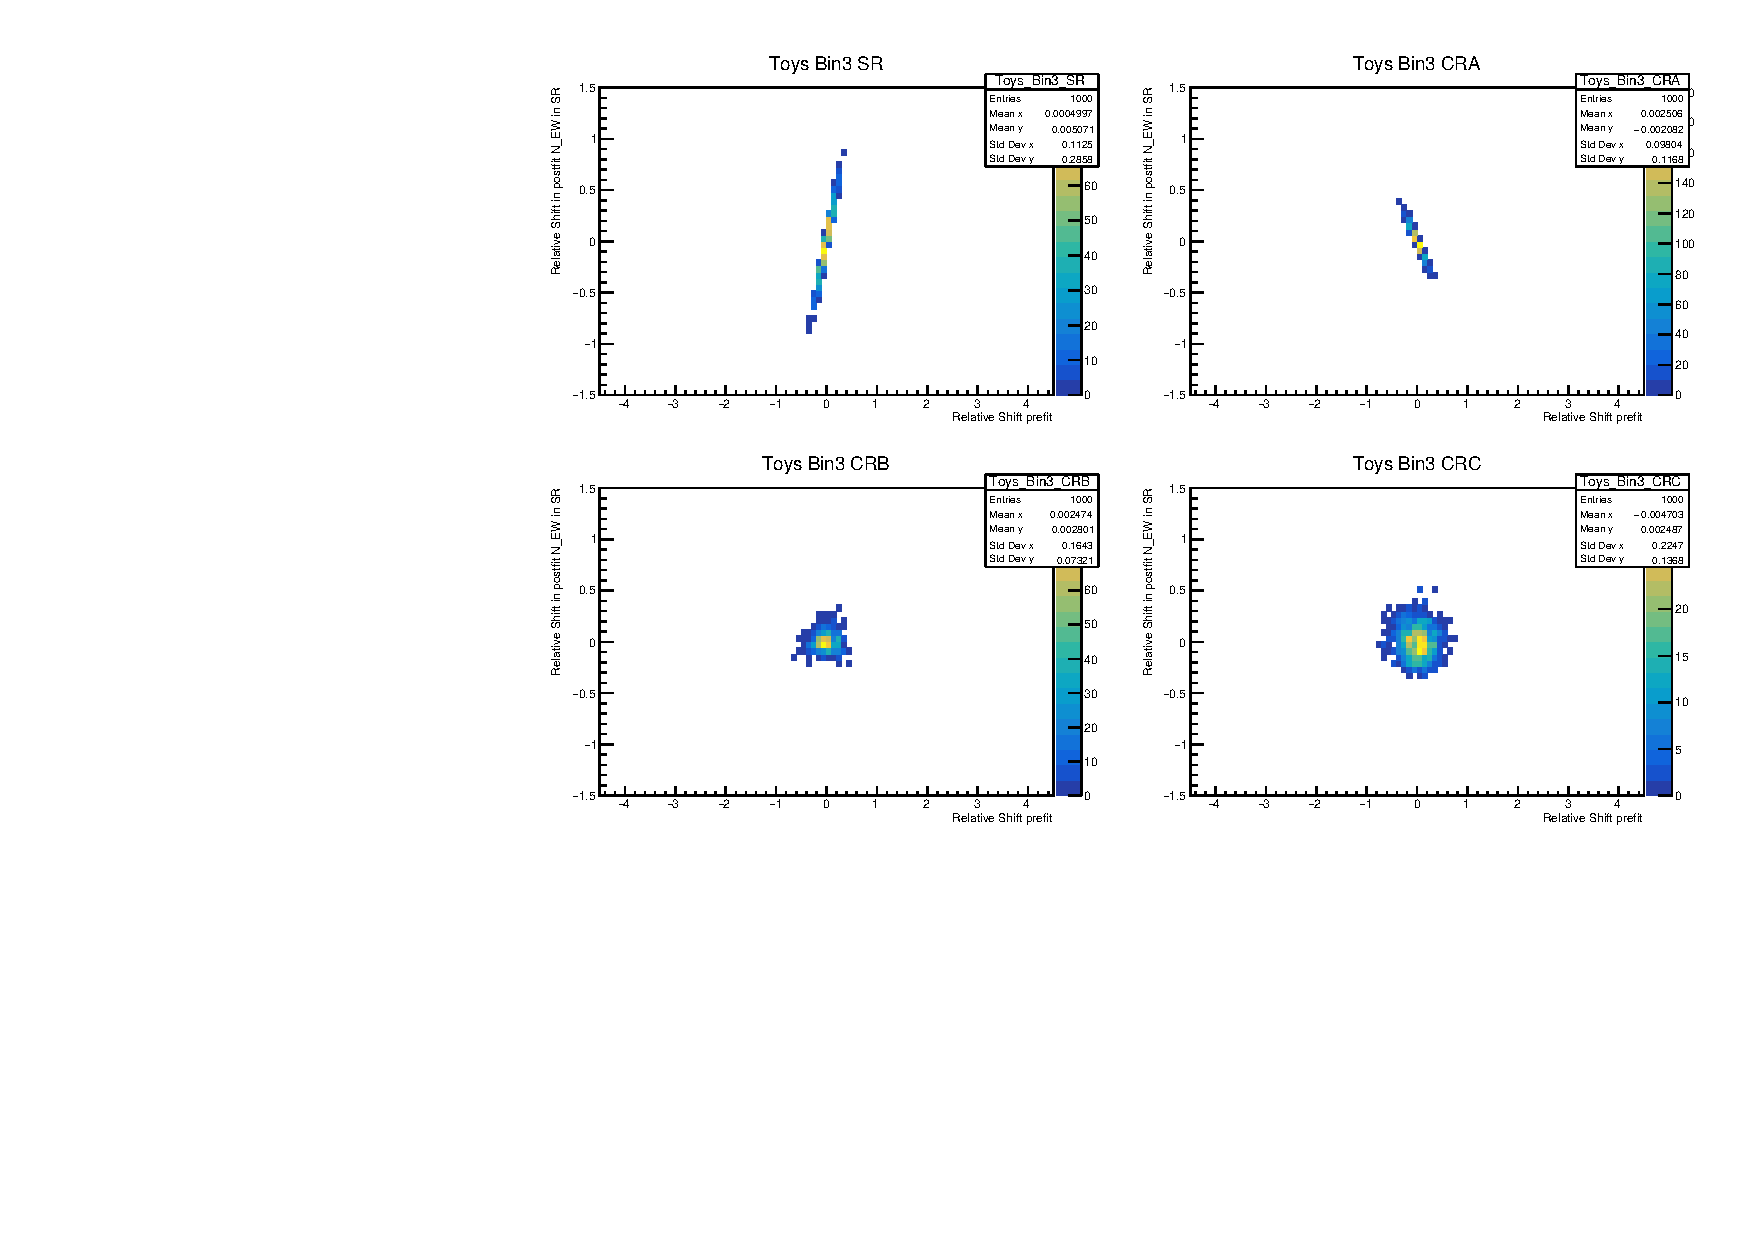
\includegraphics[width=\textwidth]{plots/diffx/instab/linearfx/instabilities_mjj_QCD_Mgraph_Signal_Sh2211_BSDATASTATS_linearfx_newbinning_sherpaasimov_bin3.pdf}
\end{figure}
\begin{figure}[H]
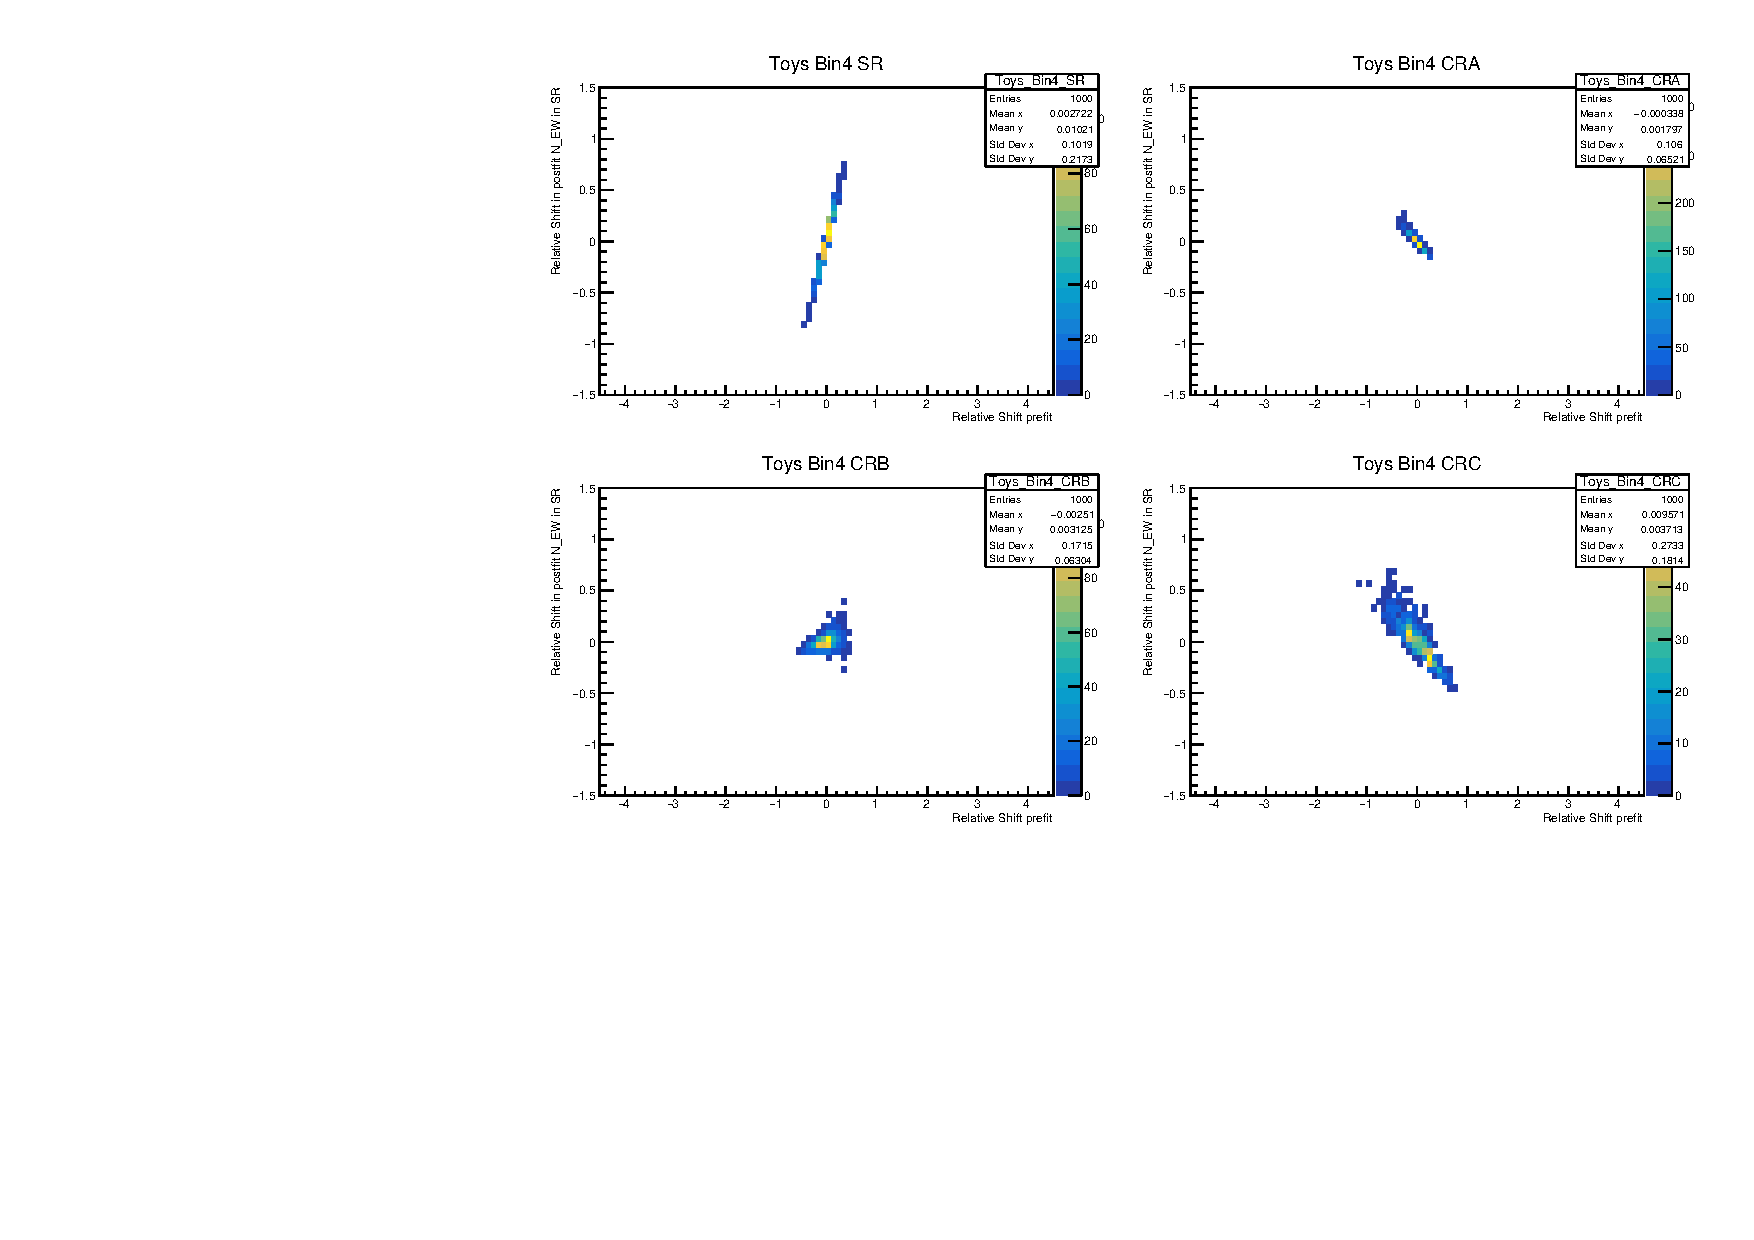
\includegraphics[width=\textwidth]{plots/diffx/instab/linearfx/instabilities_mjj_QCD_Mgraph_Signal_Sh2211_BSDATASTATS_linearfx_newbinning_sherpaasimov_bin4.pdf}
\end{figure}

\subsubsection{\mjj QCD template fluctuations, MG5 QCD in Asimov, MG5 QCD template}
\begin{figure}[H]
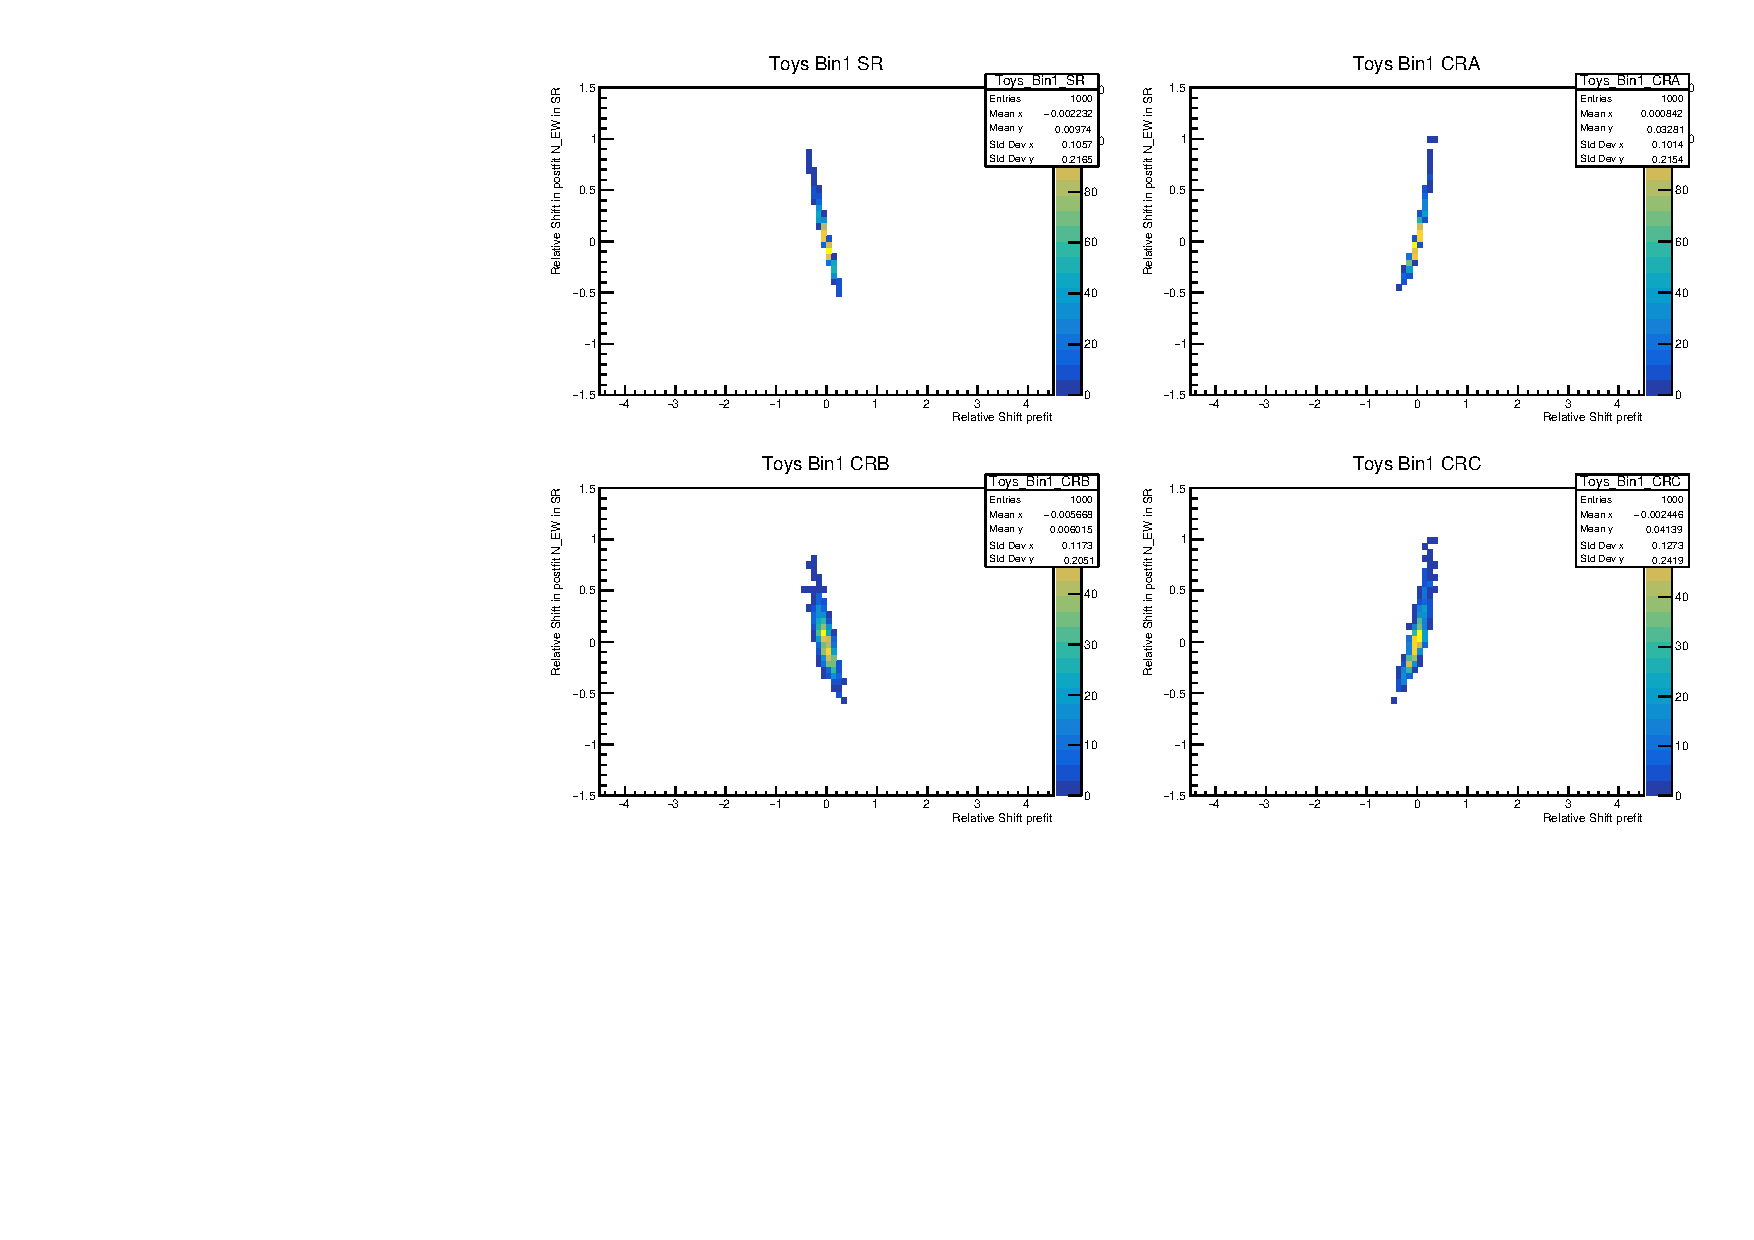
\includegraphics[width=\textwidth]{plots/diffx/instab/linearfx/instabilities_mjj_QCD_Mgraph_Signal_Sh2211_BSMCQCDSTATS_linearfx_newbinning_madgraphasimov_bin1.pdf}
\end{figure}
\begin{figure}[H]
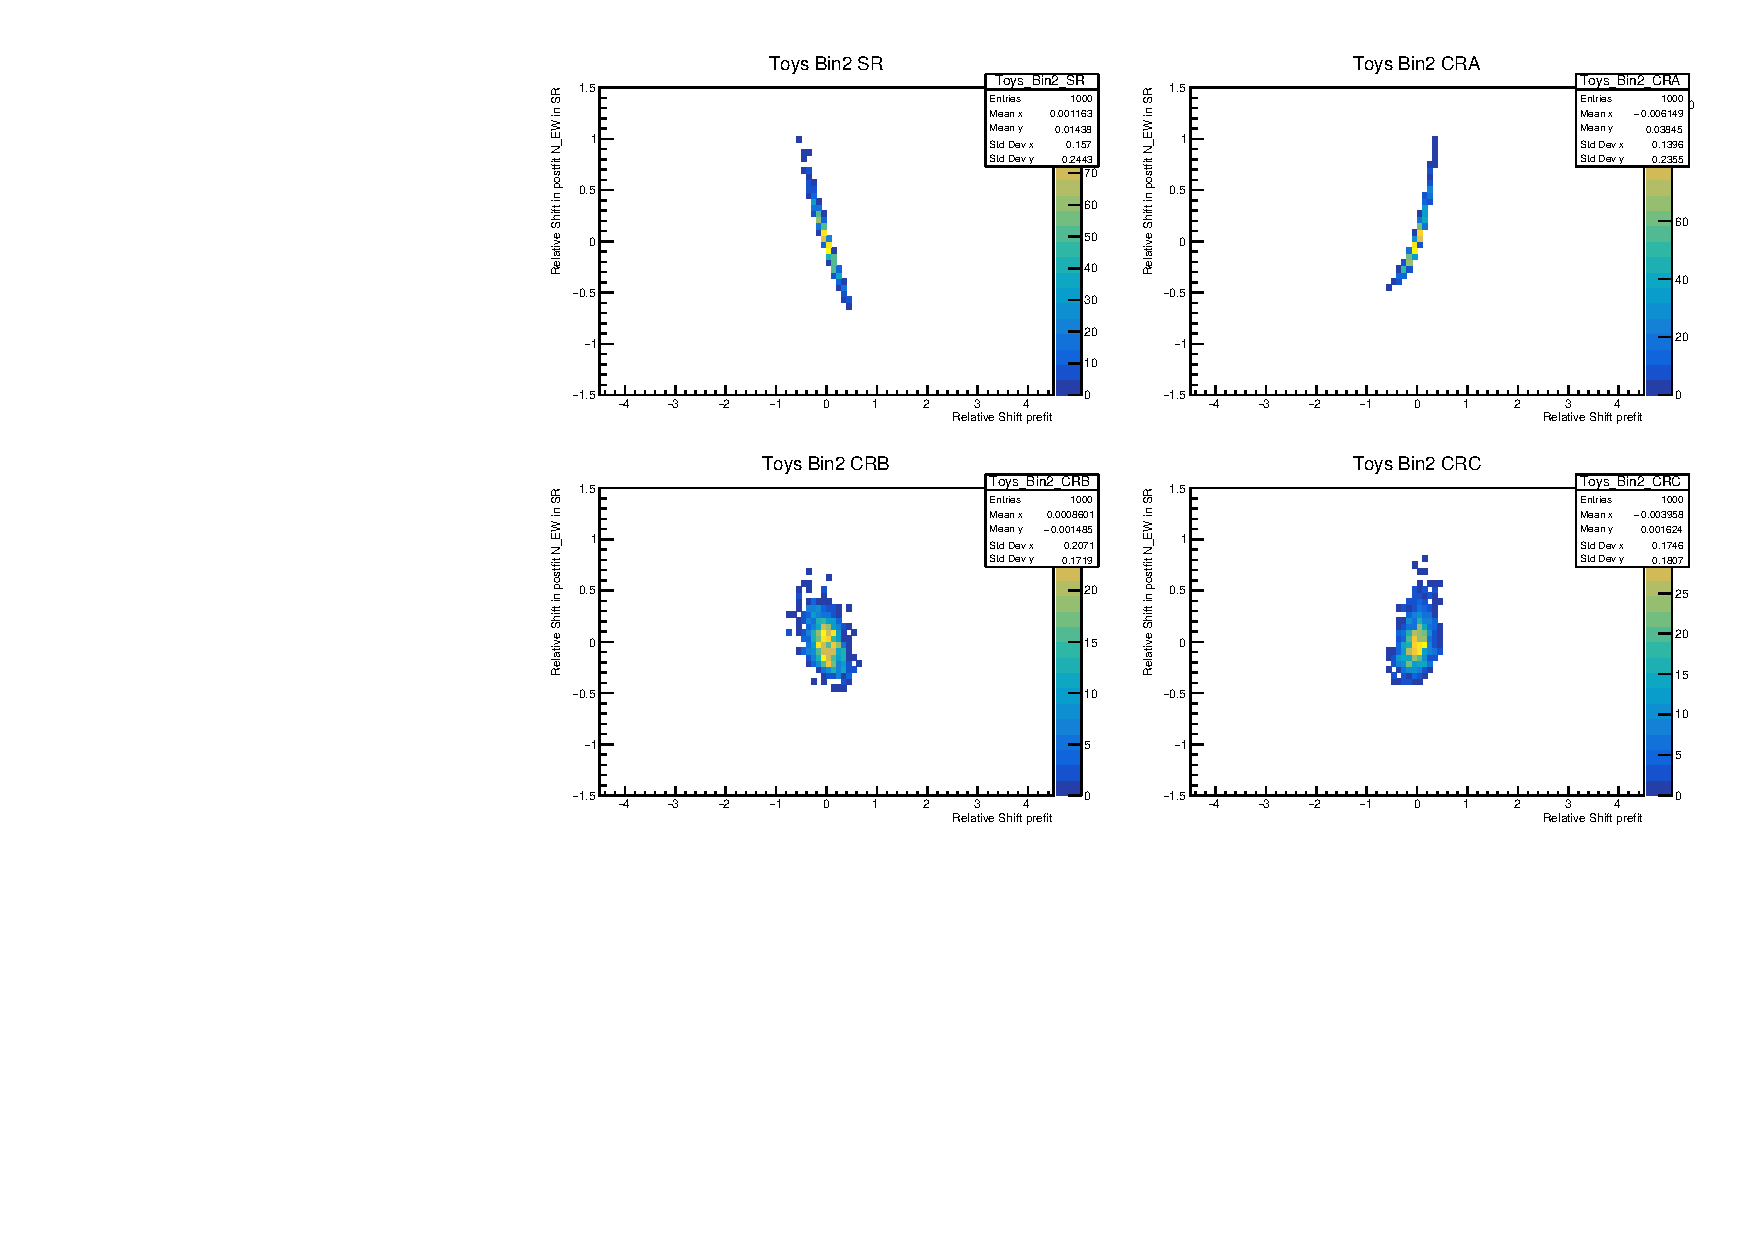
\includegraphics[width=\textwidth]{plots/diffx/instab/linearfx/instabilities_mjj_QCD_Mgraph_Signal_Sh2211_BSMCQCDSTATS_linearfx_newbinning_madgraphasimov_bin2.pdf}
\end{figure}
\begin{figure}[H]
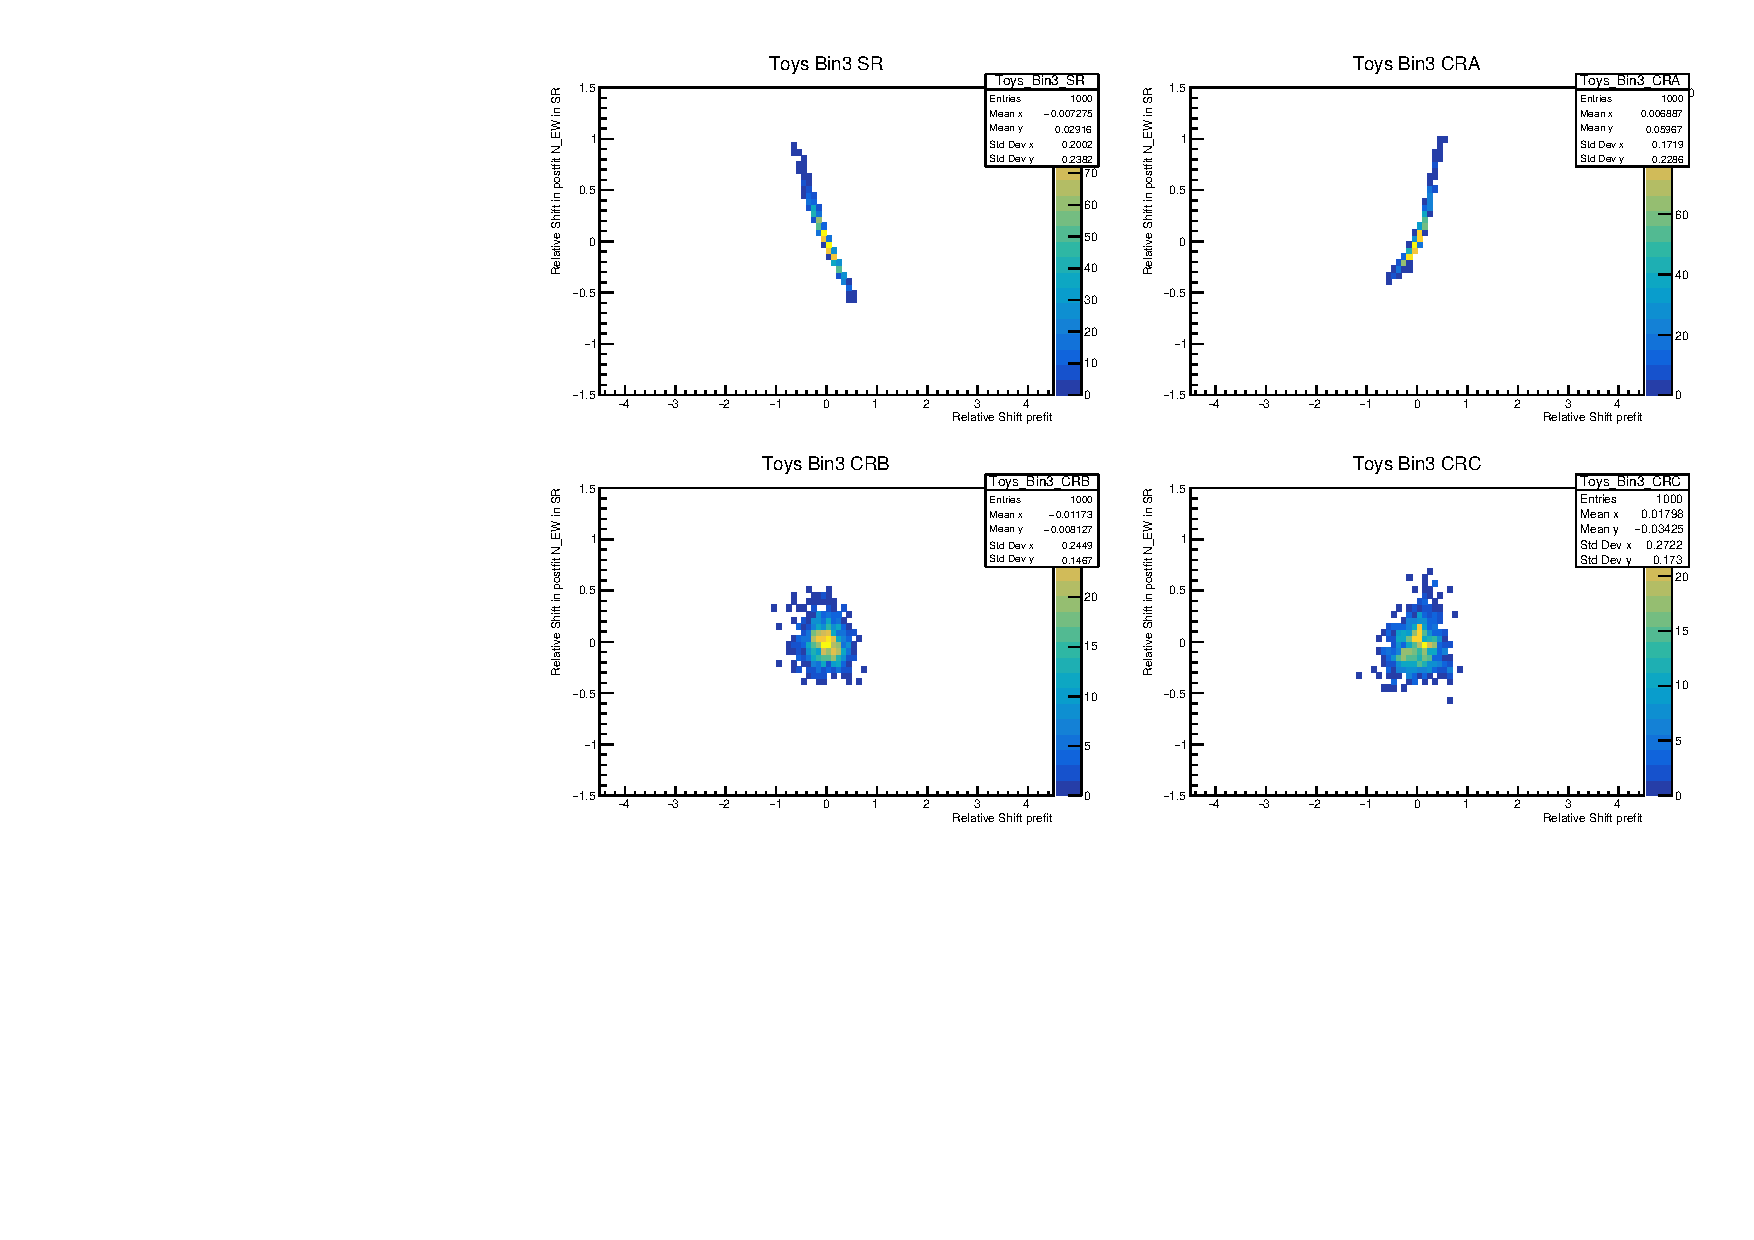
\includegraphics[width=\textwidth]{plots/diffx/instab/linearfx/instabilities_mjj_QCD_Mgraph_Signal_Sh2211_BSMCQCDSTATS_linearfx_newbinning_madgraphasimov_bin3.pdf}
\end{figure}
\begin{figure}[H]
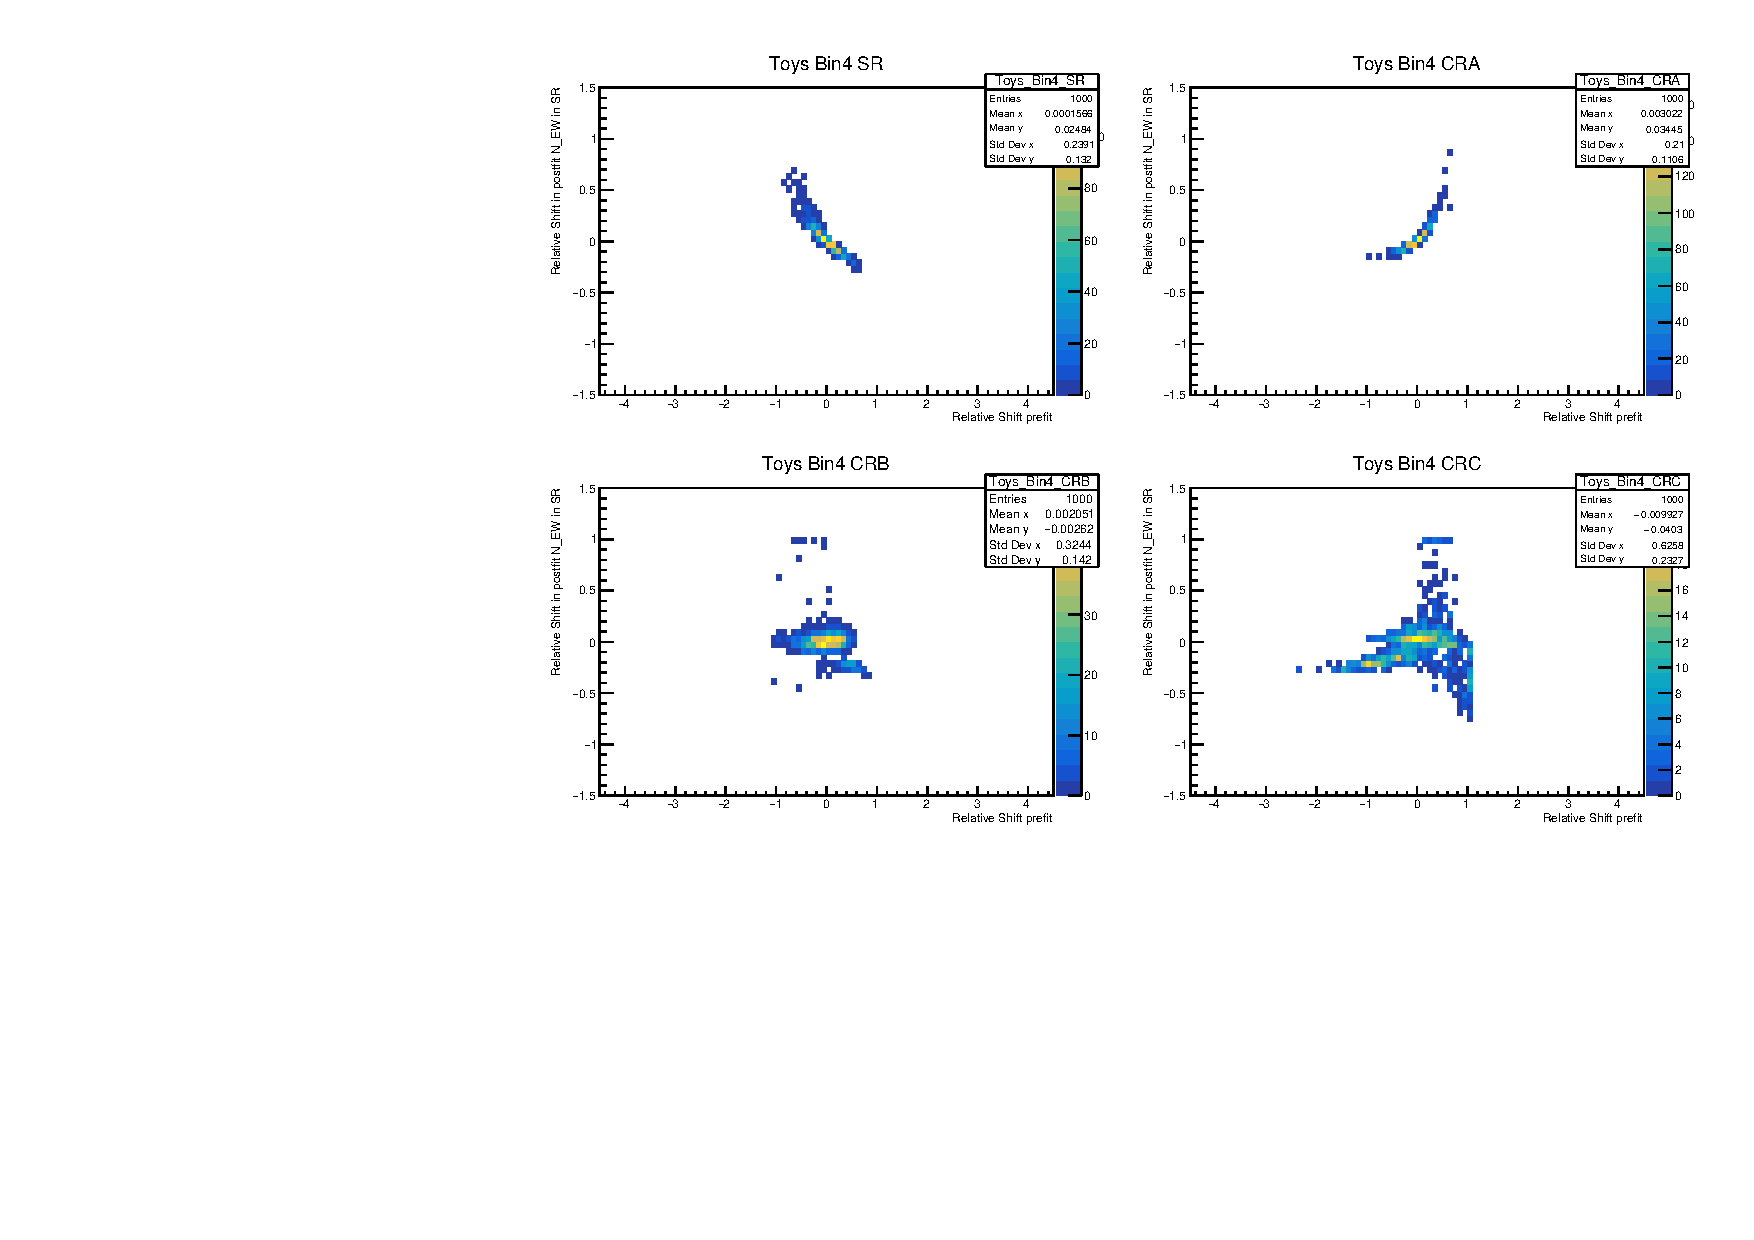
\includegraphics[width=\textwidth]{plots/diffx/instab/linearfx/instabilities_mjj_QCD_Mgraph_Signal_Sh2211_BSMCQCDSTATS_linearfx_newbinning_madgraphasimov_bin4.pdf}
\end{figure}

\subsubsection{\mjj QCD template fluctuations, Sherpa-2.2.11 QCD in Asimov, MG5 QCD template}
\begin{figure}[H]
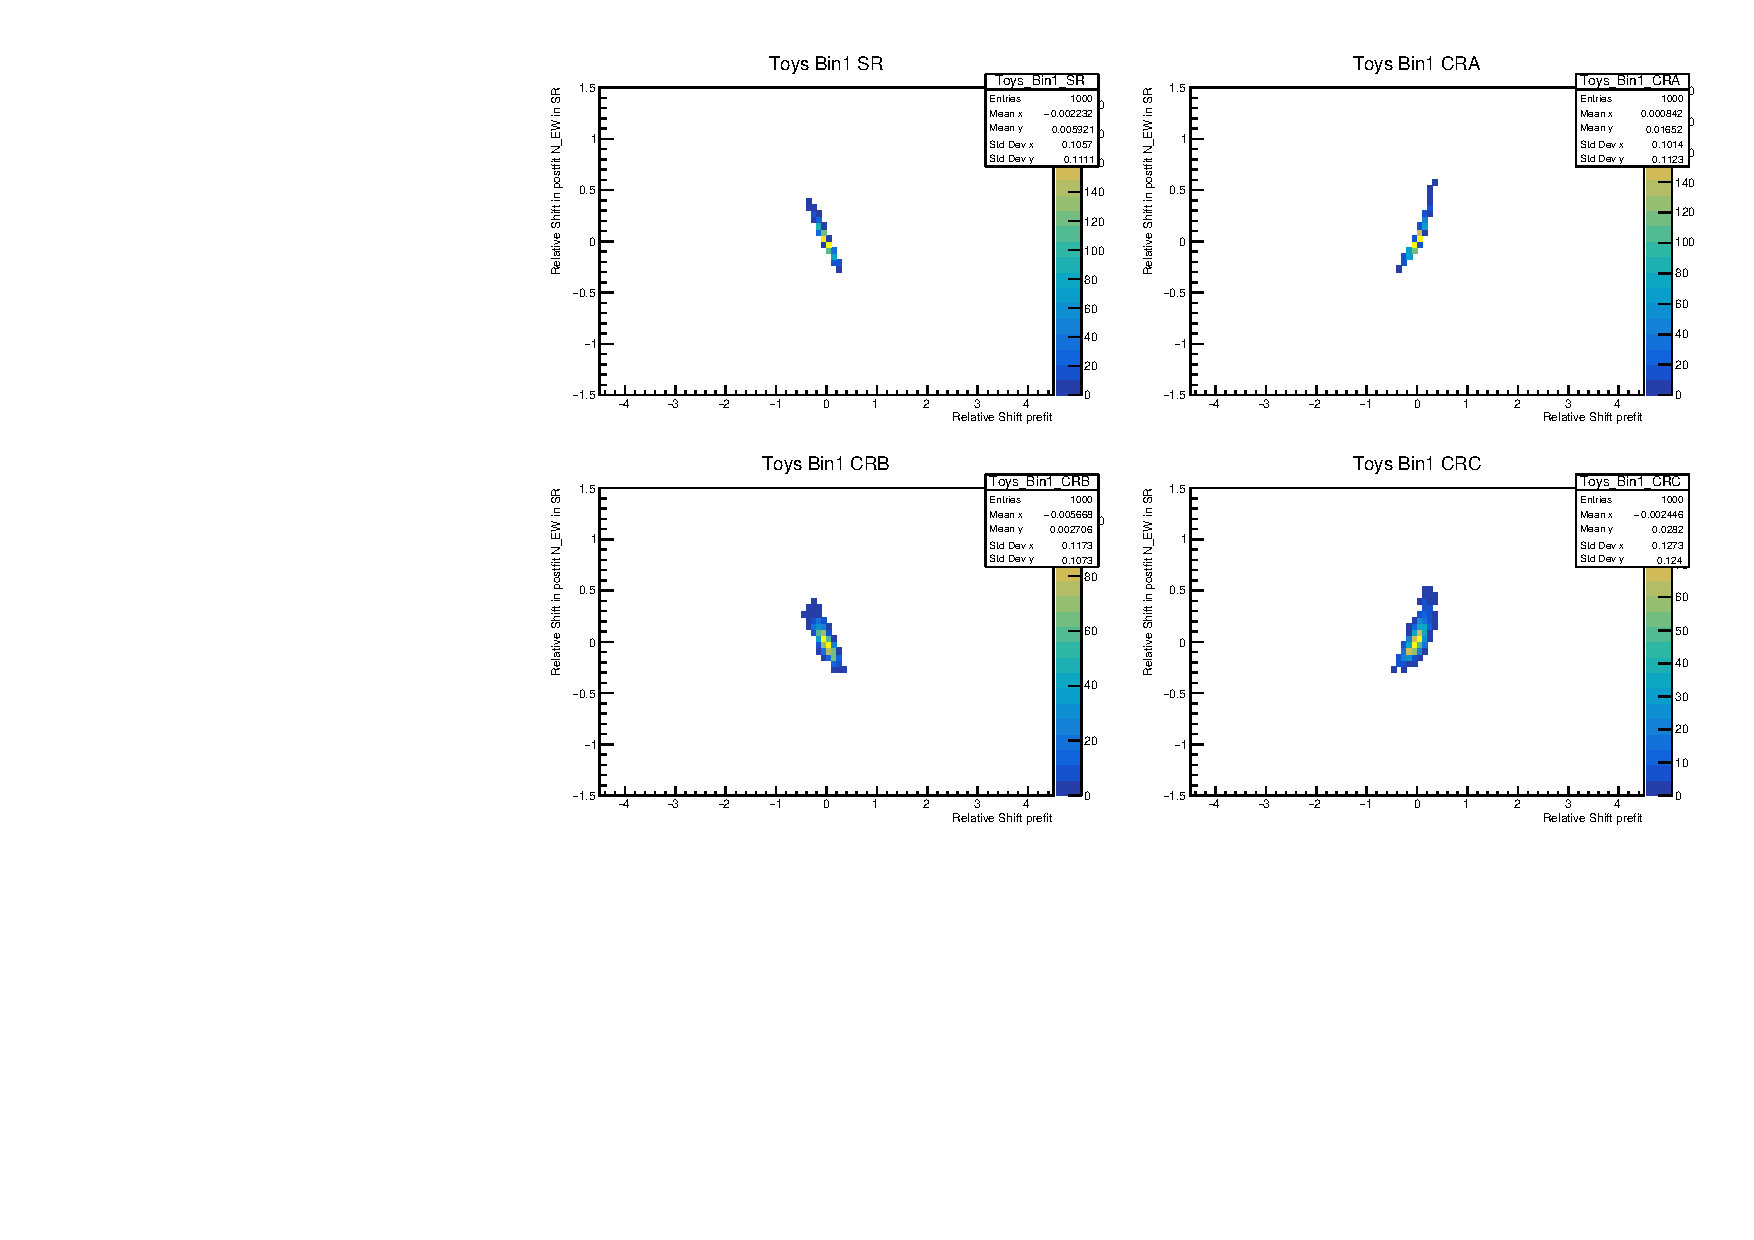
\includegraphics[width=\textwidth]{plots/diffx/instab/linearfx/instabilities_mjj_QCD_Mgraph_Signal_Sh2211_BSMCQCDSTATS_linearfx_newbinning_sherpaasimov_bin1.pdf}
\end{figure}
\begin{figure}[H]
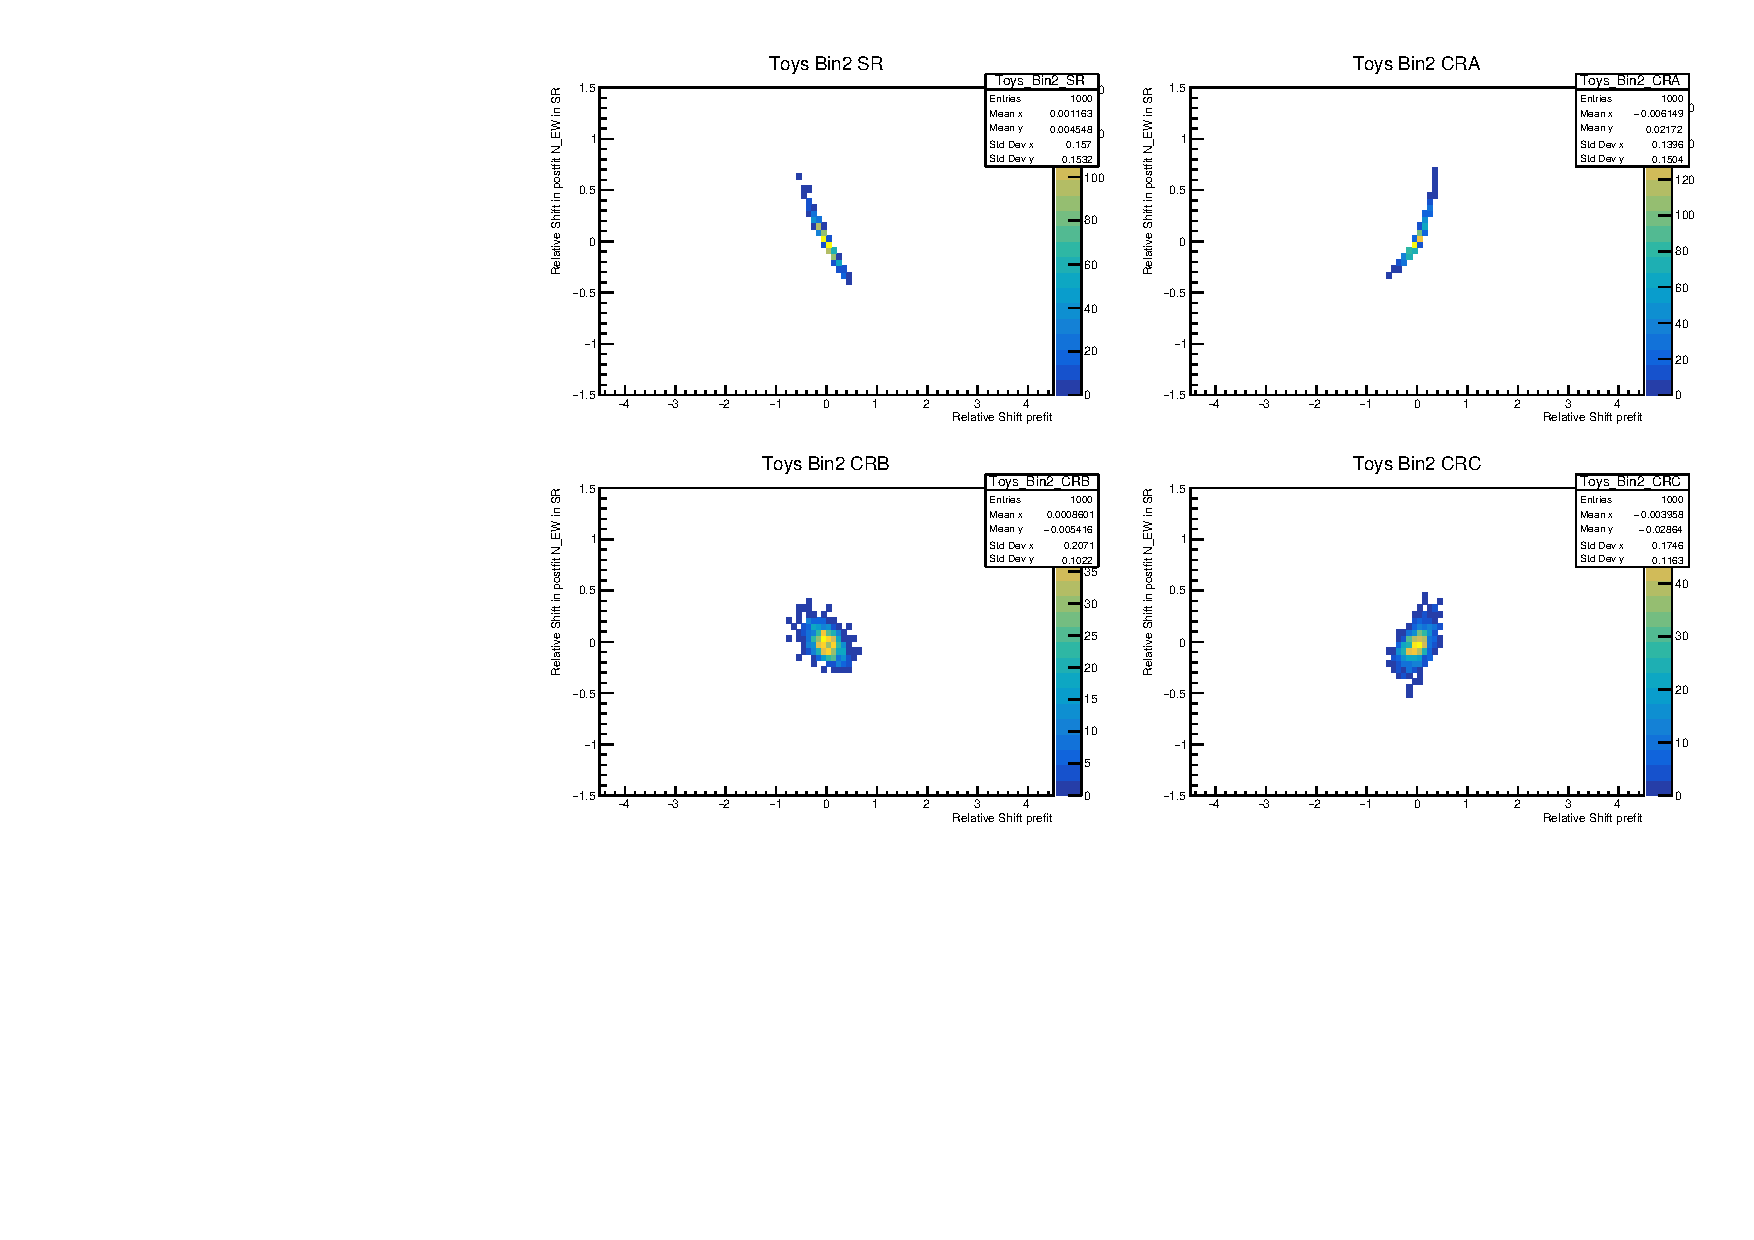
\includegraphics[width=\textwidth]{plots/diffx/instab/linearfx/instabilities_mjj_QCD_Mgraph_Signal_Sh2211_BSMCQCDSTATS_linearfx_newbinning_sherpaasimov_bin2.pdf}
\end{figure}
\begin{figure}[H]
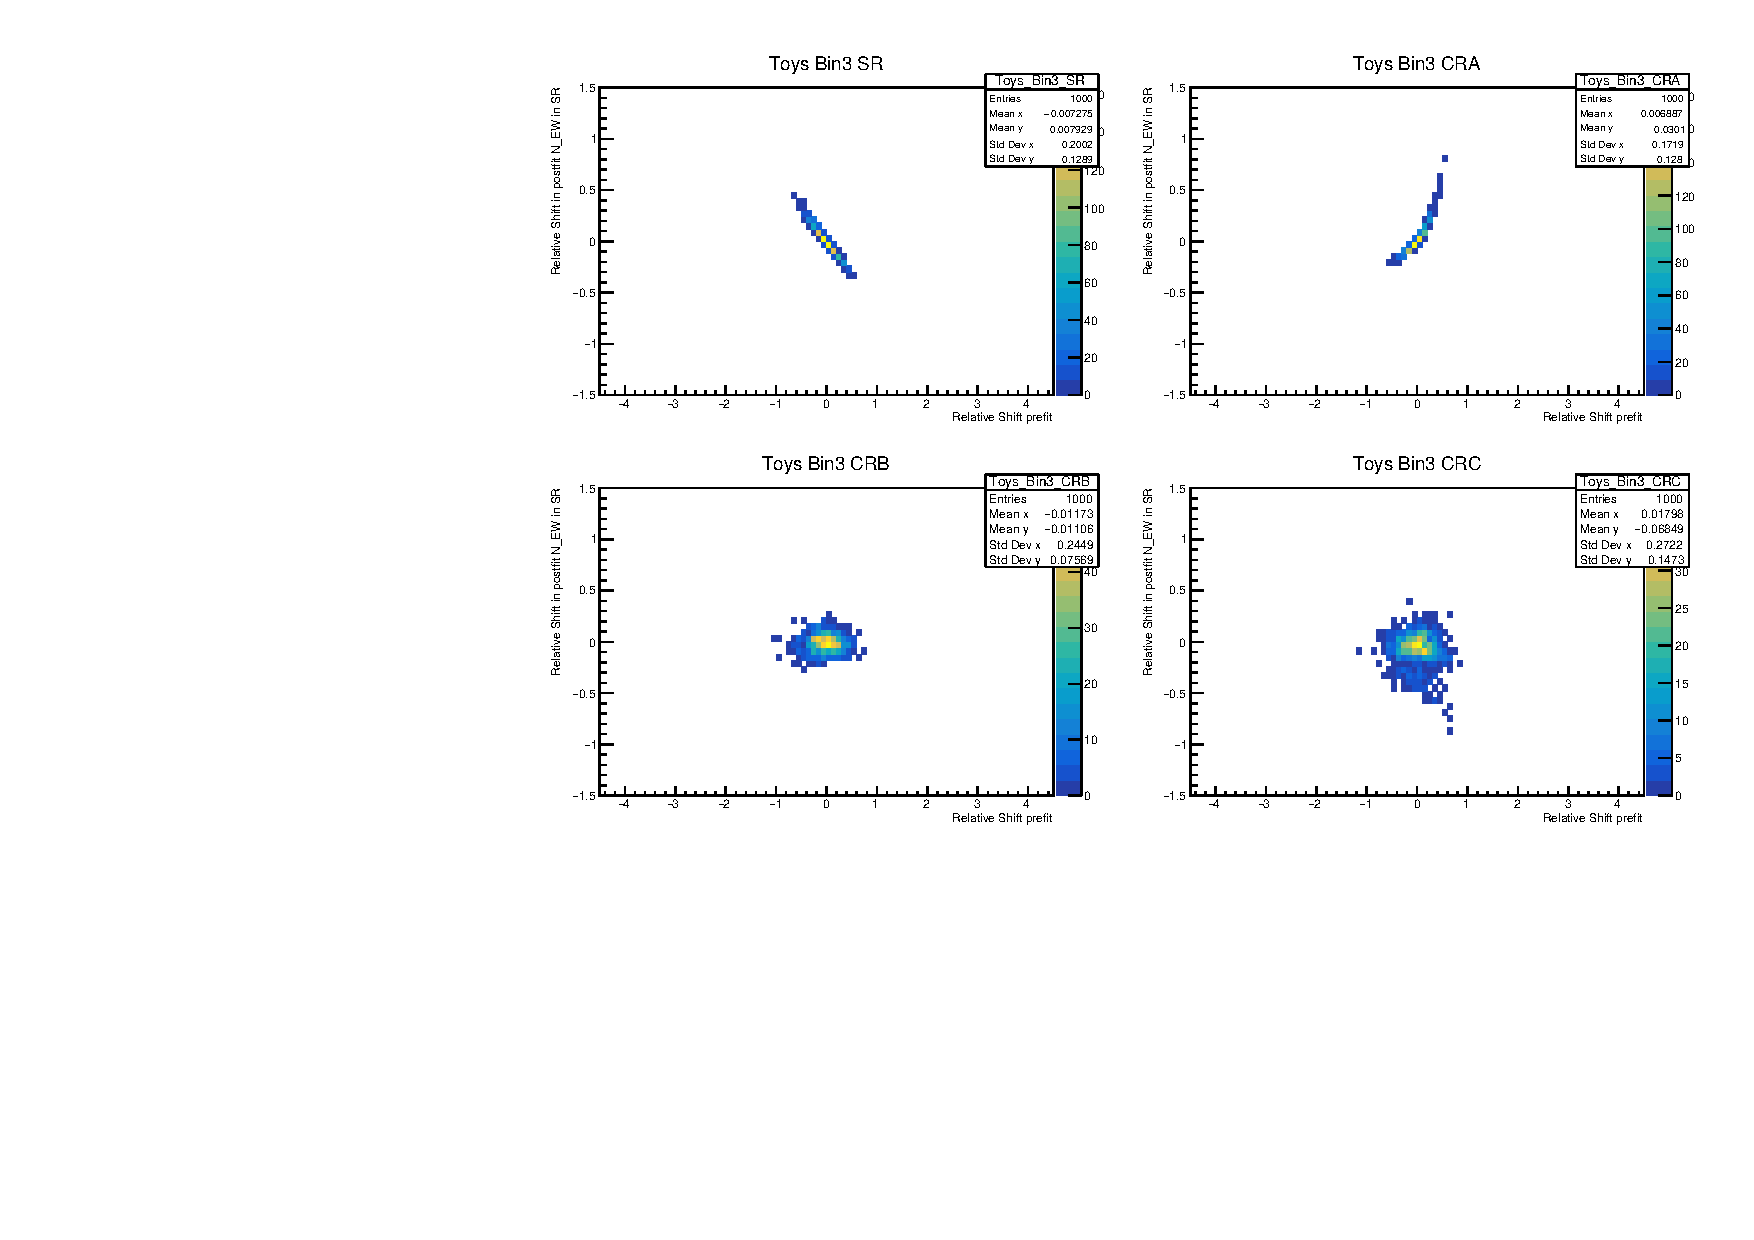
\includegraphics[width=\textwidth]{plots/diffx/instab/linearfx/instabilities_mjj_QCD_Mgraph_Signal_Sh2211_BSMCQCDSTATS_linearfx_newbinning_sherpaasimov_bin3.pdf}
\end{figure}
\begin{figure}[H]
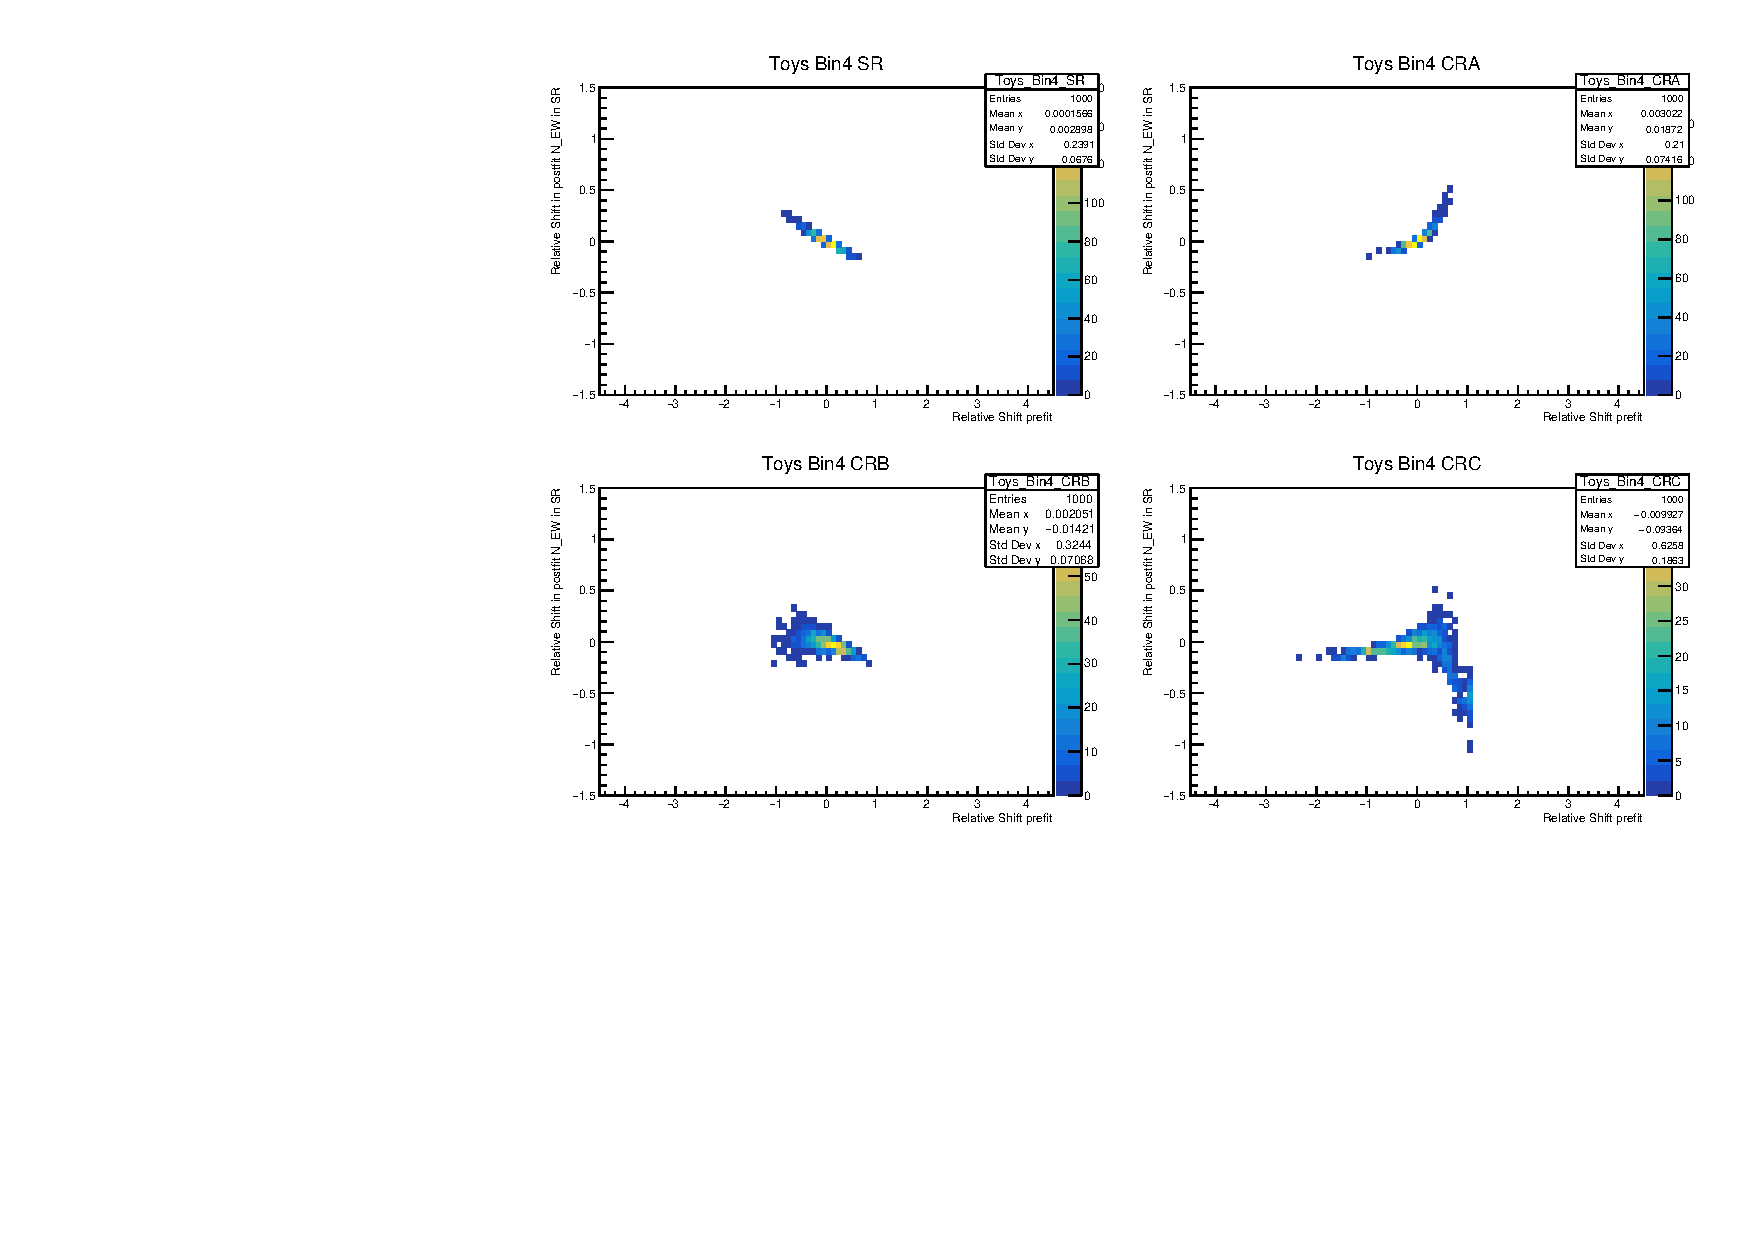
\includegraphics[width=\textwidth]{plots/diffx/instab/linearfx/instabilities_mjj_QCD_Mgraph_Signal_Sh2211_BSMCQCDSTATS_linearfx_newbinning_sherpaasimov_bin4.pdf}
\end{figure}

\subsubsection{\mjj Asimov fluctuations, MG5 QCD in Asimov, Sherpa-2.2.11 QCD template}
\begin{figure}[H]
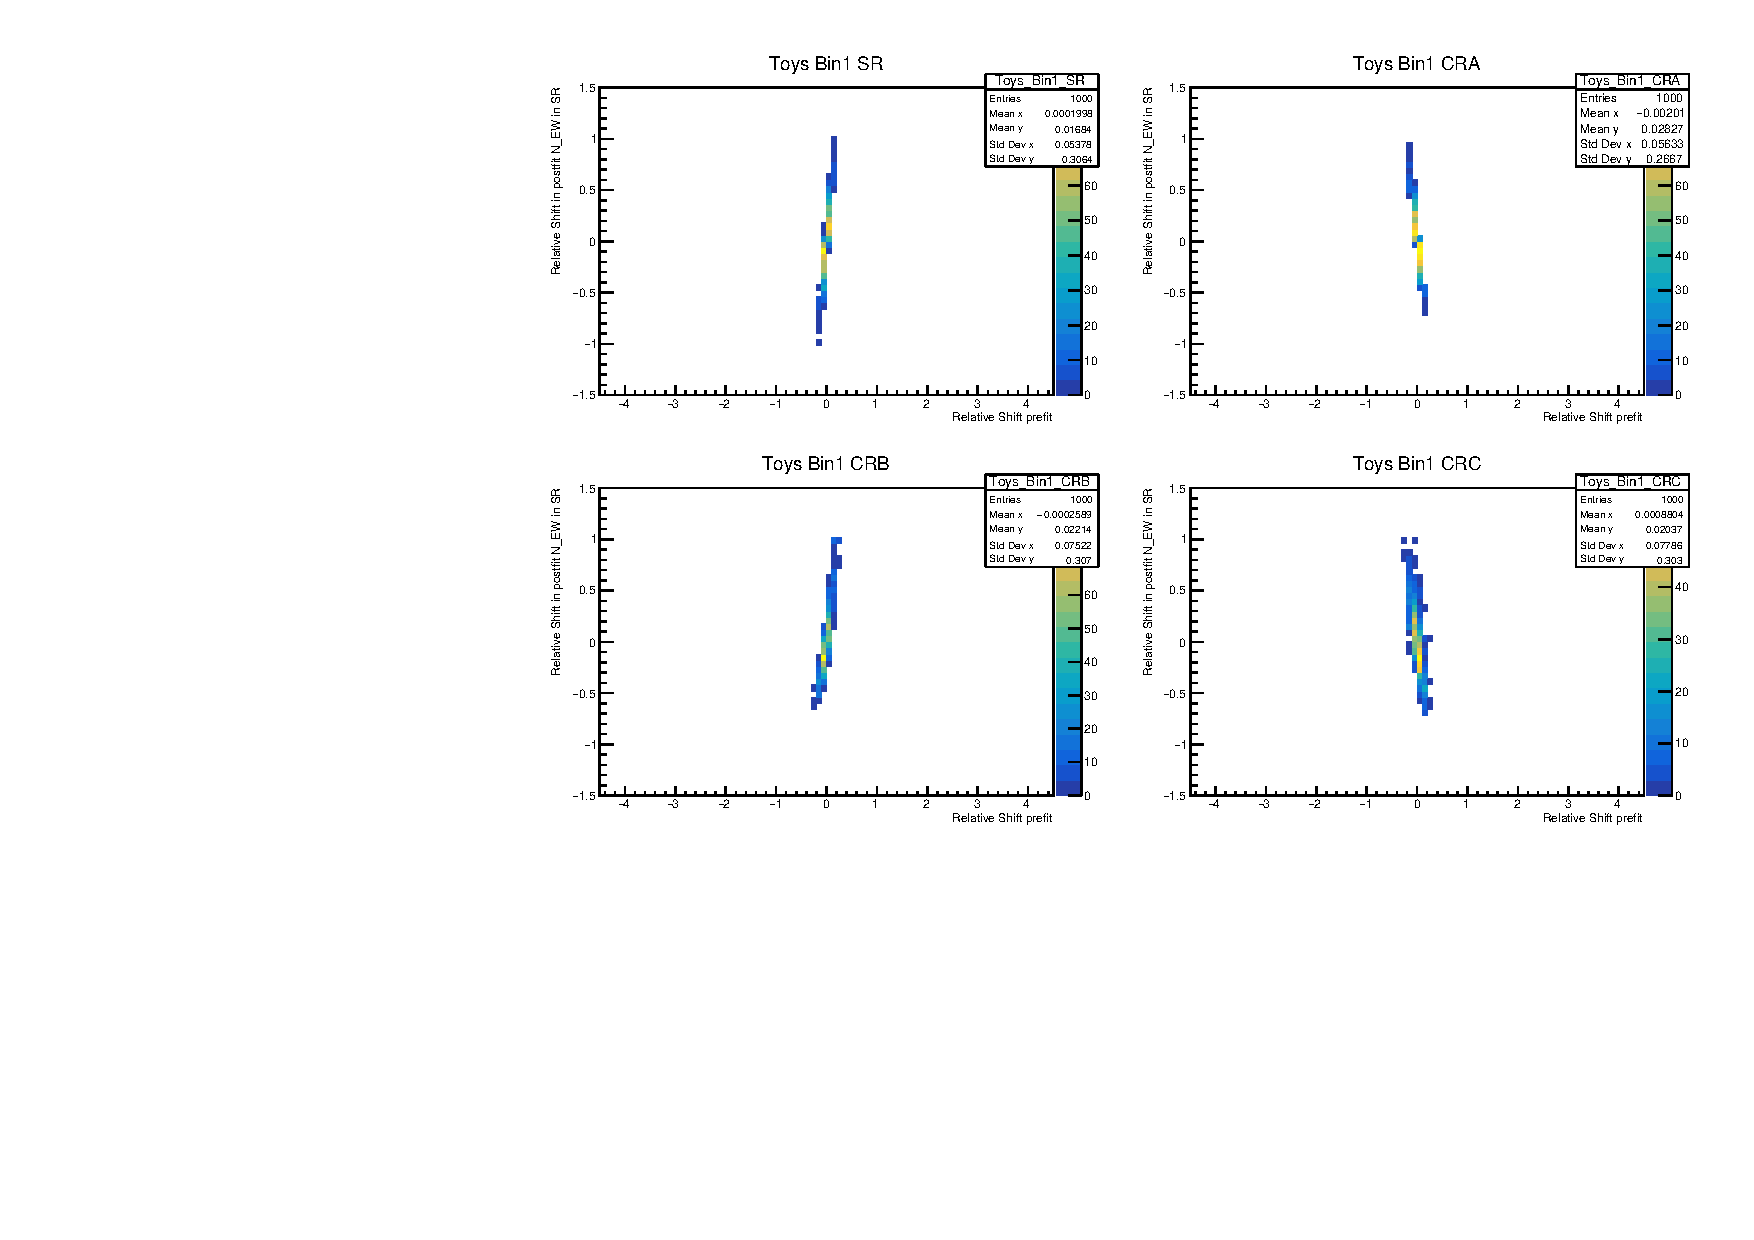
\includegraphics[width=\textwidth]{plots/diffx/instab/linearfx/instabilities_mjj_QCD_Sh2211_Signal_Sh2211_BSDATASTATS_linearfx_newbinning_madgraphasimov_bin1.pdf}
\end{figure}
\begin{figure}[H]
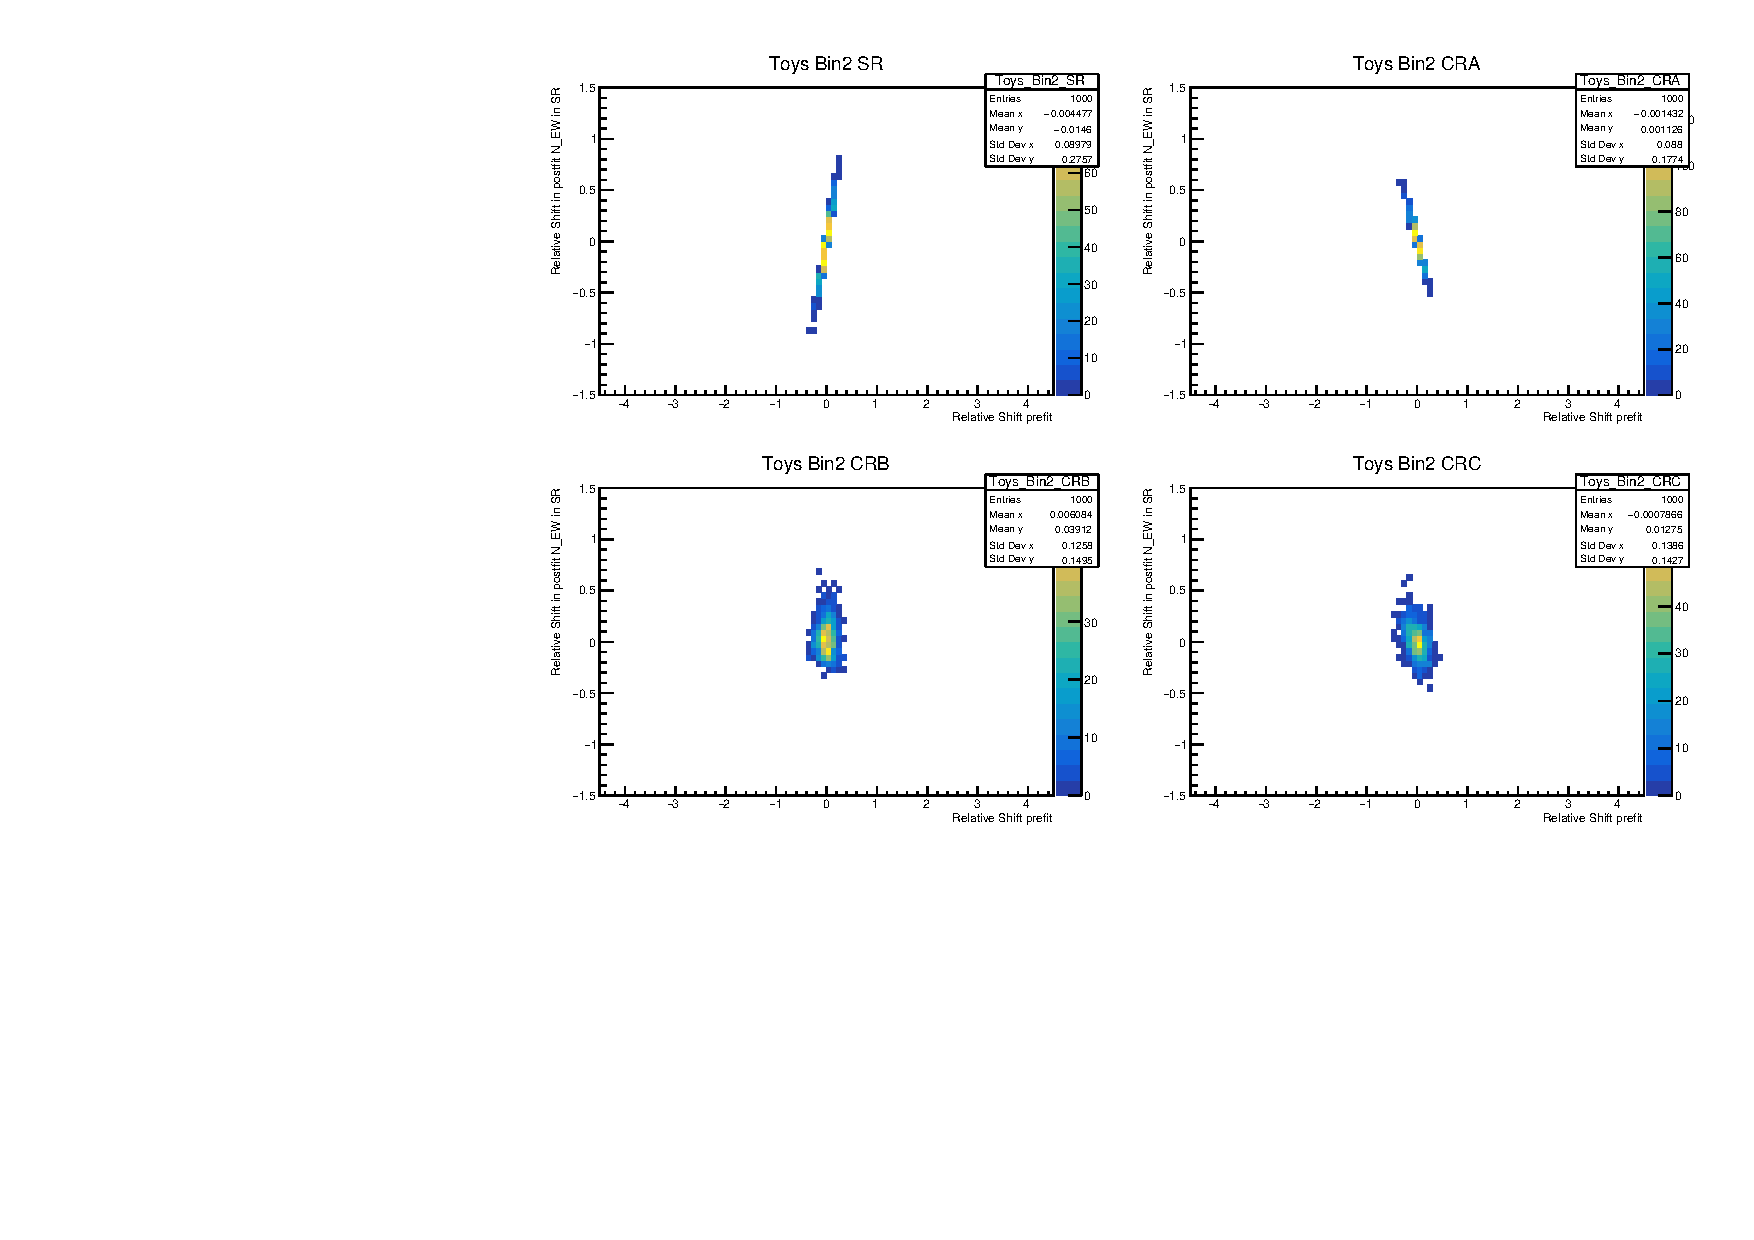
\includegraphics[width=\textwidth]{plots/diffx/instab/linearfx/instabilities_mjj_QCD_Sh2211_Signal_Sh2211_BSDATASTATS_linearfx_newbinning_madgraphasimov_bin2.pdf}
\end{figure}
\begin{figure}[H]
\includegraphics[width=\textwidth]{plots/diffx/instab/linearfx/instabilities_mjj_QCD_Sh2211_Signal_Sh2211_BSDATASTATS_linearfx_newbinning_madgraphasimov_bin3.pdf}
\end{figure}
\begin{figure}[H]
\includegraphics[width=\textwidth]{plots/diffx/instab/linearfx/instabilities_mjj_QCD_Sh2211_Signal_Sh2211_BSDATASTATS_linearfx_newbinning_madgraphasimov_bin4.pdf}
\end{figure}

\subsubsection{\mjj Asimov fluctuations, Sherpa-2.2.11 QCD in Asimov, Sherpa-2.2.11 QCD template}
\begin{figure}[H]
\includegraphics[width=\textwidth]{plots/diffx/instab/linearfx/instabilities_mjj_QCD_Sh2211_Signal_Sh2211_BSDATASTATS_linearfx_newbinning_sherpaasimov_bin1.pdf}
\end{figure}
\begin{figure}[H]
\includegraphics[width=\textwidth]{plots/diffx/instab/linearfx/instabilities_mjj_QCD_Sh2211_Signal_Sh2211_BSDATASTATS_linearfx_newbinning_sherpaasimov_bin2.pdf}
\end{figure}
\begin{figure}[H]
\includegraphics[width=\textwidth]{plots/diffx/instab/linearfx/instabilities_mjj_QCD_Sh2211_Signal_Sh2211_BSDATASTATS_linearfx_newbinning_sherpaasimov_bin3.pdf}
\end{figure}
\begin{figure}[H]
\includegraphics[width=\textwidth]{plots/diffx/instab/linearfx/instabilities_mjj_QCD_Sh2211_Signal_Sh2211_BSDATASTATS_linearfx_newbinning_sherpaasimov_bin4.pdf}
\end{figure}

\subsubsection{\mjj QCD template fluctuations, MG5 QCD in Asimov, Sherpa-2.2.11 QCD template}
\begin{figure}[H]
\includegraphics[width=\textwidth]{plots/diffx/instab/linearfx/instabilities_mjj_QCD_Sh2211_Signal_Sh2211_BSMCQCDSTATS_linearfx_newbinning_madgraphasimov_bin1.pdf}
\end{figure}
\begin{figure}[H]
\includegraphics[width=\textwidth]{plots/diffx/instab/linearfx/instabilities_mjj_QCD_Sh2211_Signal_Sh2211_BSMCQCDSTATS_linearfx_newbinning_madgraphasimov_bin2.pdf}
\end{figure}
\begin{figure}[H]
\includegraphics[width=\textwidth]{plots/diffx/instab/linearfx/instabilities_mjj_QCD_Sh2211_Signal_Sh2211_BSMCQCDSTATS_linearfx_newbinning_madgraphasimov_bin3.pdf}
\end{figure}
\begin{figure}[H]
\includegraphics[width=\textwidth]{plots/diffx/instab/linearfx/instabilities_mjj_QCD_Sh2211_Signal_Sh2211_BSMCQCDSTATS_linearfx_newbinning_madgraphasimov_bin4.pdf}
\end{figure}

\subsubsection{\mjj QCD template fluctuations, Sherpa-2.2.11 QCD in Asimov, Sherpa-2.2.11 QCD template}
\begin{figure}[H]
\includegraphics[width=\textwidth]{plots/diffx/instab/linearfx/instabilities_mjj_QCD_Sh2211_Signal_Sh2211_BSMCQCDSTATS_linearfx_newbinning_sherpaasimov_bin1.pdf}
\end{figure}
\begin{figure}[H]
\includegraphics[width=\textwidth]{plots/diffx/instab/linearfx/instabilities_mjj_QCD_Sh2211_Signal_Sh2211_BSMCQCDSTATS_linearfx_newbinning_sherpaasimov_bin2.pdf}
\end{figure}
\begin{figure}[H]
\includegraphics[width=\textwidth]{plots/diffx/instab/linearfx/instabilities_mjj_QCD_Sh2211_Signal_Sh2211_BSMCQCDSTATS_linearfx_newbinning_sherpaasimov_bin3.pdf}
\end{figure}
\begin{figure}[H]
\includegraphics[width=\textwidth]{plots/diffx/instab/linearfx/instabilities_mjj_QCD_Sh2211_Signal_Sh2211_BSMCQCDSTATS_linearfx_newbinning_sherpaasimov_bin4.pdf}
\end{figure}

\section{Different Significance Thresholds\label{sec:appendix:sigthresholds}}
This appendix shows the final systematic uncertainties on \new with significance thresholds set at $\sigma_{\text{thresh}}=1.0$ and $\sigma_{\text{thresh}}=1.6$.
\subsection{$\sigma_{\text{thresh}}=1.0$}

\begin{figure}[H]
    \centering
    \includegraphics[width=0.49\textwidth]{plots/diffx/sigthresholds/1p0/Systematic_Uncertainties_data_mjj_3cr_QCD_Sh2211_1p0sigma.pdf}
    \includegraphics[width=0.49\textwidth]{plots/diffx/sigthresholds/1p0/Systematic_Uncertainties_data_jj_pt_3cr_QCD_Sh2211_1p0sigma.pdf}
    \includegraphics[width=0.49\textwidth]{plots/diffx/sigthresholds/1p0/Systematic_Uncertainties_data_jj_dphi_3cr_QCD_Sh2211_1p0sigma.pdf}
    \includegraphics[width=0.49\textwidth]{plots/diffx/sigthresholds/1p0/Systematic_Uncertainties_data_lep_pt_3cr_QCD_Sh2211_1p0sigma.pdf}
    \includegraphics[width=0.49\textwidth]{plots/diffx/sigthresholds/1p0/Systematic_Uncertainties_data_lepgam_dphi_3cr_QCD_Sh2211_1p0sigma.pdf}
    \includegraphics[width=0.49\textwidth]{plots/diffx/sigthresholds/1p0/Systematic_Uncertainties_data_ly_m_3cr_QCD_Sh2211_1p0sigma.pdf}
    \caption{Systematic uncertainties with significance threshold of $\sigma_{\text{thresh}}=1.0$.\label{fig:app:thresholdone}}
\end{figure}

\subsection{$\sigma_{\text{thresh}}=1.6$}

\begin{figure}[H]
    \centering
    \includegraphics[width=0.49\textwidth]{plots/diffx/sigthresholds/1p6/Systematic_Uncertainties_data_mjj_3cr_QCD_Sh2211_1p6sigma.pdf}
    \includegraphics[width=0.49\textwidth]{plots/diffx/sigthresholds/1p6/Systematic_Uncertainties_data_jj_pt_3cr_QCD_Sh2211_1p6sigma.pdf}
    \includegraphics[width=0.49\textwidth]{plots/diffx/sigthresholds/1p6/Systematic_Uncertainties_data_jj_dphi_3cr_QCD_Sh2211_1p6sigma.pdf}
    \includegraphics[width=0.49\textwidth]{plots/diffx/sigthresholds/1p6/Systematic_Uncertainties_data_lep_pt_3cr_QCD_Sh2211_1p6sigma.pdf}
    \includegraphics[width=0.49\textwidth]{plots/diffx/sigthresholds/1p6/Systematic_Uncertainties_data_lepgam_dphi_3cr_QCD_Sh2211_1p6sigma.pdf}
    \includegraphics[width=0.49\textwidth]{plots/diffx/sigthresholds/1p6/Systematic_Uncertainties_data_ly_m_3cr_QCD_Sh2211_1p6sigma.pdf}
    \caption{Systematic uncertainties with significance threshold of $\sigma_{\text{thresh}}=1.0$.\label{fig:app:thresholdonepsix}}
\end{figure}